\section{Évaluation de l'hypothèse sur les coûts}
\label{section:4.3-HYPOTHESE-COUTS}

	%%%
	%%% Introduction / Transition.
	%%%
	Dans les deux sections précédentes, nous avons estimé le paramétrage du \texttt{Clustering Interactif} le plus efficient pour atteindre $90$\% de \texttt{v-measure} avec la vérité terrain, correspondant à ce que nous appelons une annotation partielle.
	Toutefois, pour compléter l'étude de faisabilité technique de notre méthode, nous devons nous intéresser aux coûts (matériel et humain) à investir pour atteindre notre objectif.
	Nous aimerions donc vérifier l'hypothèse suivante :
	
	%%%
	%%% Formulation des hypothèses.
	%%%
	\begin{tcolorbox}[
		title=\faVial~\textbf{Hypothèse sur les coûts}~\faVial,
		colback=colorTcolorboxHypothesis!15,
		colframe=colorTcolorboxHypothesis!75,
		width=\linewidth
	]
		% Hypothèse.
		\textguillemets{\textbf{
			Il est possible d'estimer les coûts nécessaires d'une méthodologie d'annotation basée sur le \texttt{Clustering Interactif} pour obtenir une base d'apprentissage exploitable.
			Nous étudions en particulier les coûts relatifs au temps d'annotation, au temps de calculs des algorithmes, ainsi que la durée totale de la méthode en fonction de la taille du jeu de données.
		}} \\
		
		% Figure.
		La \textsc{Figure~\ref{figure:4.3-HYPOTHESE-COUTS}} illustre cette hypothèse et la perspective de pouvoir caractériser la qualité de la base d'apprentissage en cours de construction en fonction d'un coût temporel au lieu d'un nombre abstrait d'itérations de la méthode. 
		%
		\begin{figure}[H]  % keep [H] to be in the tcolorbox.
			\centering
			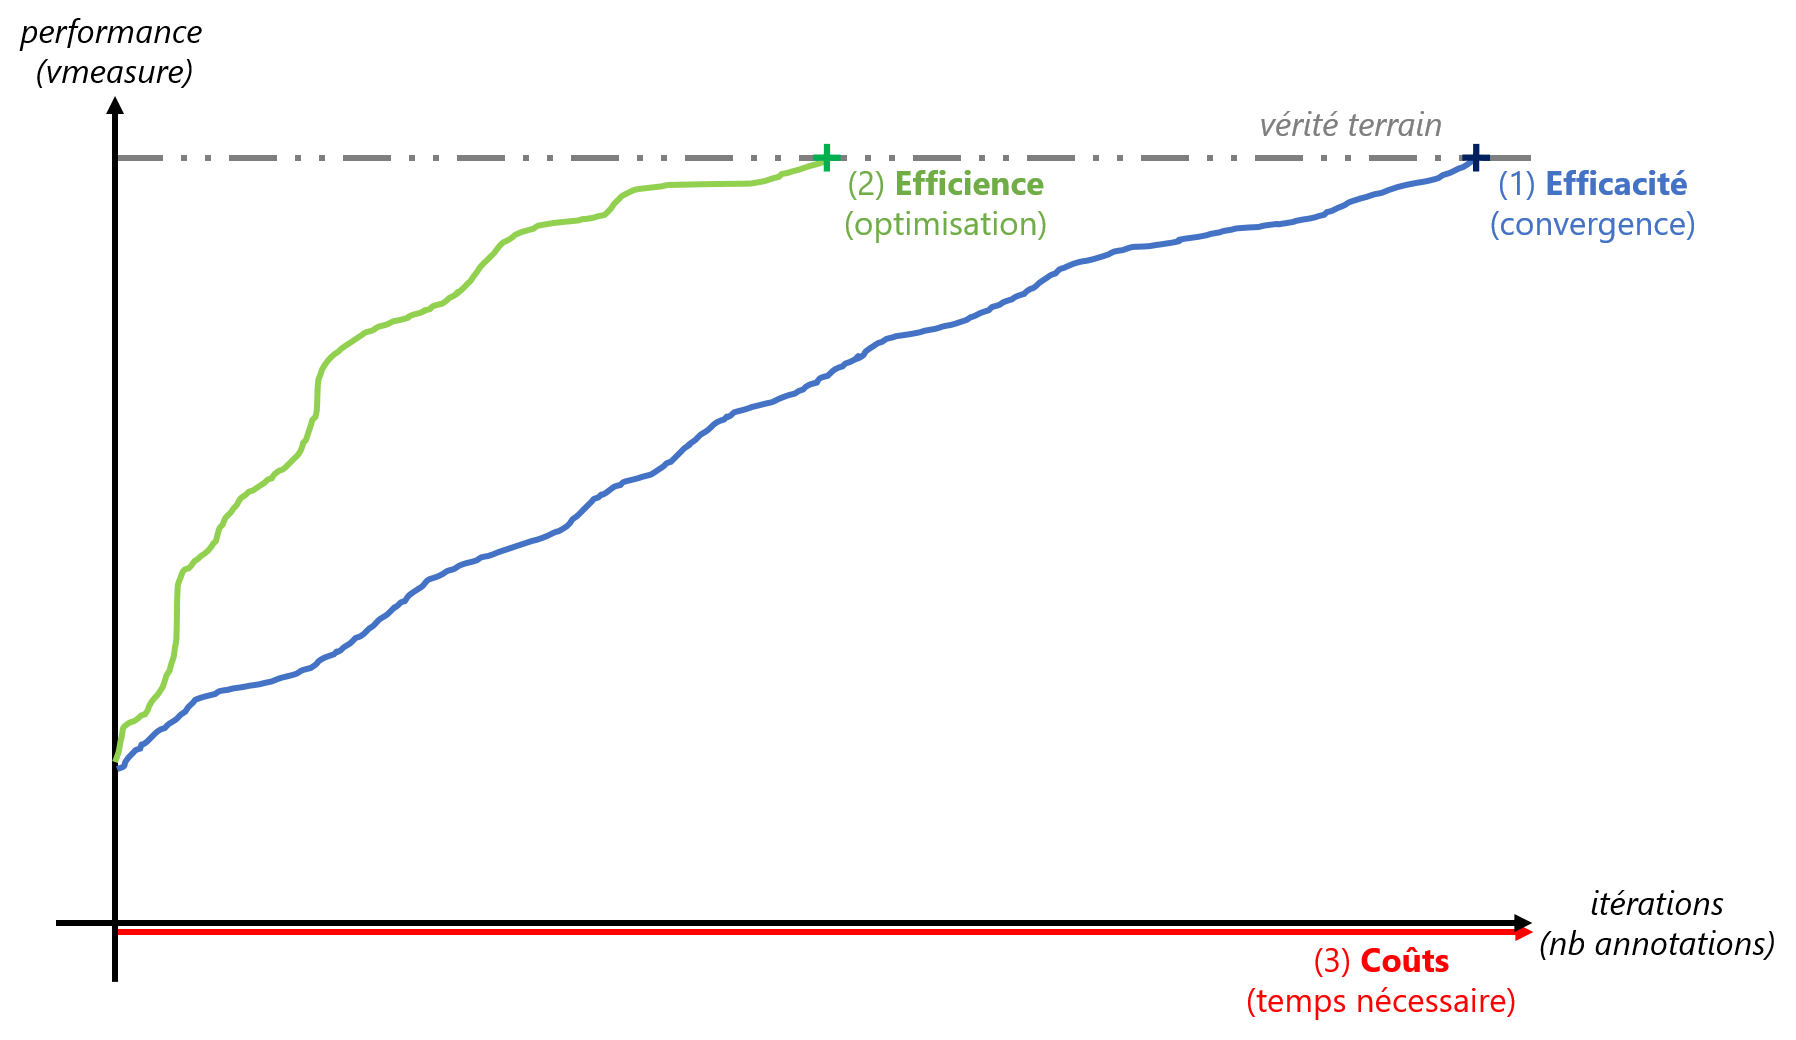
\includegraphics[width=0.95\textwidth]{figures/hypotheses-03-couts}
			\caption{
				Illustration des études réalisées sur le \texttt{Clustering Interactif} (\textit{étape 3/6}) en schématisant l'évolution de la performance (\textit{accord avec la vérité terrain calculé en v-measure}) d'une base d'apprentissage en cours de construction en fonction du coût temporel de la méthode (\textit{temps nécessaire à l'expert métier et à la machine}).
			}
			\label{figure:4.3-HYPOTHESE-COUTS}
		\end{figure}
	\end{tcolorbox}

	% Résumé des études.
	Afin de vérifier cette hypothèse, nous organisons plusieurs expériences pour simuler et déterminer ces durées :
	\begin{itemize}
		\item une étude du \textbf{temps d'annotation} par un expert métier, temps mesuré lors d'une expérience d'annotation de contraintes faisant intervenir plusieurs opérateurs (cf. \textsc{Section~\ref{section:4.3.1-ETUDE-COUTS-TEMPS-ANNOTATION}}) ;
		\item une étude du \textbf{temps de calcul} des algorithmes, temps modélisé en exécutant les différentes implémentations du \texttt{Clustering Interactif} avec diverses valeurs d'arguments (cf. \textsc{Section~\ref{section:4.3.2-ETUDE-COUTS-TEMPS-CALCUL}}) ; et
		\item une étude du \textbf{nombre de contraintes} nécessaires en fonction du nombre de données à traiter, nombre estimé en simulant la création d'une base d'annotation avec notre méthodologie sur des jeux de données de différentes tailles (cf. \textsc{Section~\ref{section:4.3.3-ETUDE-COUT-NOMBRE-CONTRAINTES}}).
	\end{itemize}
	Nous exposons nos conclusions sur l'estimation du \textbf{temps total} à investir et réalisons une comparaison avec une organisation plus traditionnelle d'un projet d'annotation en \textsc{Section~\ref{section:4.3.4-ETUDE-COUTS-TOTAL}}.
	
	
	%%%
	%%% Subsection 4.3.1: Étude du temps d'annotation nécessaire pour traiter un lot de contraintes en chronométrant des opérateurs en situation réelle
	%%%
	\subsection{Étude du temps d'annotation nécessaire pour traiter un lot de contraintes en chronométrant des opérateurs en situation réelle}
	\label{section:4.3.1-ETUDE-COUTS-TEMPS-ANNOTATION}
		
		% Objectif de l'expérience.
		Nous voulons estimer le temps nécessaire à un opérateur pour annoter un lot de contraintes.
		Pour cela, nous allons chronométrer plusieurs experts métiers en train d'annoter un même échantillon et modéliser le nombre de contraintes par minute, ainsi que son évolution au cours de plusieurs sessions d'annotation.
		De plus, nous aimerions aussi confirmer que l'ajout de contraintes dans notre contexte s'apparente à une tâche "intuitive", c'est-à-dire que l'annotation se fait dans la réaction et non dans la réflexion (voir \cite{kahneman:2011:thinking-fast-slow} qui distingue un \textit{système 1} intuitif, rapide, de l'ordre de l'émotion, et un \textit{système 2} plus lent, logique et réfléchi).
		Pour ce faire, nous estimons grossièrement le temps nécessaire à l'annotation réactive d'une contrainte, nous le comparons au temps moyen estimé lors de notre expérience, et nous nous demandons si la différence observée peut cacher un mécanisme cognitif plus complexe.
	
		%%% Protocole expérimental.
		\subsubsection{Protocole expérimental}
			
			% Axiome.
			\begin{leftBarWarning}
				Dans cette étude, nous supposons que les annotateurs de l'expérience connaissent parfaitement le domaine traité dans le jeu de données, et qu'ils sont capables de caractériser sans ambiguïté la similitude entre deux données issues de cet ensemble.
				Afin de pourvoir faire cette hypothèse forte, et ainsi limiter les bruits dans l'analyse des résultats, le jeu de données devra traiter d'un sujet de culture générale (ne nécessitant donc pas de connaissance particulière) et des réviseurs supprimeront en amont et d'un commun accord les données trop spécifiques ou trop ambiguës.
			\end{leftBarWarning}
			
			% Pseudo-code.
			Pour résumer le protocole expérimental que nous détaillons ci-dessous, une description en pseudo-code est disponible dans l'\textsc{Algorithme~\ref{algorithm:4.3.1-ETUDE-COUTS-TEMPS-ANNOTATION-PROTOCOLE}}.

			\begin{algorithm}
				\KwData{jeu de données annotées (vérité terrain)}
				\KwIn{plusieurs réviseurs, plusieurs annotateurs}
				%
				\textbf{initialisation}: définir et revoir le jeu de données entre réviseurs \;
				\textbf{échantillonnage}: sélectionner une base de contraintes avec \texttt{samp.rand.full} \;
				\textbf{temps théorique}: estimation du temps nécessaire à l'annotation d'une contrainte \;
				\ForEach{annotateur}{
					 \While{la base de contraintes n'a pas été entièrement annotée}{
						\textbf{chronomètre}: \textbf{START} \;
						\textbf{annotation}: annoter une partie des contraintes \;
						\textbf{revue}: revue des contraintes en conflits d'annotation \;
						\textbf{chronomètre}: \textbf{STOP} \;
						\textbf{mesure}: estimer la différence de chronomètre pour cette session \;
					}
				}
				\textbf{analyse}: modéliser le temps d'annotation d'un lot de contraintes \;
				%
				\KwResult{modélisation du temps d'annotation d'un lot de contraintes}
				%
				\caption{\textit{
					Description en pseudo-code du protocole expérimental de l'étude du temps d'annotation d'un lot de contraintes par plusieurs experts métiers en situation réelle.
				}}
				\label{algorithm:4.3.1-ETUDE-COUTS-TEMPS-ANNOTATION-PROTOCOLE}
			\end{algorithm}
			
			% Détails de l'expérience : préparation du jeu de données.
			Nous allons procéder en plusieurs étapes.
			D'abord, il faut choisir un jeu de données approprié : pour valider notre hypothèse forte sur les compétences de nos annotateurs, nous cherchons un jeu de données traitant d'un sujet de culture générale.
			Pour cette expérience, nous avons donc choisi \texttt{MLSUM} : une collecte d'articles de journaux, classés par catégorie de publication et décrits par leur titre et leur résumé.
			Nous nous intéressons ici à la tâche de classification d'un titre d'article en fonction de sa catégorie de publication.
			Comme certains titres peuvent porter à confusion (un titre d'article n'étant pas toujours explicite sur son contenu), deux réviseurs (\textit{une Data Scientist et moi-même}) sont chargés de choisir les données les plus explicites sur un échantillon d'un millier de données représentatives des catégories les plus communes.
			L'échantillon résultant, noté \texttt{MLSUM FR Train Subset (v1.0.0-schild)}, est composé de $744$ titres d'articles rédigés en français et répartis en $14$ classes (\textit{économie}, \textit{sport}, ...).
			Pour plus de détails, consulter l'\textsc{Annexe~\ref{annex:A.2-DATASET-MLSUM-SUBSET-SCHILD}}.
			
			% Détails de l'expérience : sélection des contraintes à annoter.
			À partir de ces données, nous sélectionnons un lot de $1~000$ contraintes à annoter.
			Comme nous nous intéressons exclusivement au temps d'annotation pour cette expérience (et que nous ne regardons pas le nombre d'itérations de la méthode), nous utilisons l'échantillonnage purement aléatoire (\texttt{samp.rand.full}).
			L'analyse de l'accord inter-annotateurs sera réalisé en \textsc{Section~\ref{section:4.6.1-ETUDE-ROBUSTESSE-SCORE-ACCORD}}.
			
			% Détails de l'expérience : estimation du temps théorique nécessaire à l'annotation d'une contrainte.
			Sur la base de cet échantillon, nous pouvons approximer le temps théorique nécessaire à l'annotation d'une contrainte à $6.8$ secondes.
			En effet, il faut d'abord considérer la taille moyenne des titres d'article à lire et en déduire le temps dédié à la lecture des deux textes de la contrainte.
			En utilisant l'approximation d'une lecture silencieuse par un adulte à $238$ mots par minute (\cite{brysbaert:2019:how-many-words}) et en mesurant la taille moyenne des titres d'article à $10.1$ mots, nous en déduisons que le temps de lecture d'un texte est environ de $2.55$ secondes.
			Ensuite, il convient d'intégrer la durée de traitement cognitif requis pour estimer si les deux phrases sont similaires ou discordantes.
			À cet effet, nous retenons $1$ seconde \footnote{
				Nous pourrions faire le parallèle avec la composante \texttt{P600} communément admise en neuroscience pour caractériser la réaction provoquée par la dissonance grammaticale ou syntaxique d'une phrase.
				Nous arrondissons à $1$ seconde pour garder une marge d'erreur.
			} (\cite{purves-brannon:2013:principles-cognitive-neuroscience})
			en admettant que cette tâche est rapide.
			Enfin, nous ajoutons $1$ seconde supplémentaire pour représenter la réaction motrice (clic de bouton) et le délai applicatif (rechargement de la page).
			Au total, nous obtenons ainsi un temps d'annotation moyen de $7$ secondes.
			Bien entendu, cette durée reste approximative, mais elle nous permet de discuter de l'ordre de grandeur à manipuler durant l'annotation.
			
			% Détails de l'expérience : annotations et consignes.
			Ensuite, un groupe de $14$ annotateurs vont annoter la sélection de $1~000$ contraintes en plusieurs sessions.
			Les directives données aux opérateurs sont les suivantes:
			\begin{itemize}
				\item \textbf{Contexte de l'opérateur} :
				\textguillemets{\textit{Vous êtes des \textbf{experts de la presse et de l'actualité}.
					Vous voulez classer des articles dans des catégories en fonction de leur titre.
					Vous ne savez pas précisément quelles catégories vous allez utiliser pour classer vos articles.
					Mais vous savez \textbf{caractériser la similitude} entre deux articles
				}}.
				\item \textbf{Contexte du jeu de données} :
				\textguillemets{\textit{Le thème concerne les catégories d'articles de presse.
					La vérité terrain contient entre $10$ et $20$ catégories parmi les plus communes de la presse.
					La vérité terrain contient entre $30$ et $100$ articles par catégorie.
					Vous \textbf{pouvez regarder le jeu de données non annoté} autant que vous le voulez (disponible dans l'onglet \texttt{TEXTS} de l'application)
				}}.
				\item \textbf{Objectif de l'expérience} :
				\textguillemets{\textit{
					Je veux savoir le temps nécessaire pour annoter un certain nombre de contraintes.
					Autrement dit : \textbf{pour annoter 1000 contraintes, combien de temps me faut-il ?}
				}}.
				\item \textbf{Consignes d'annotations} :
				\textguillemets{\textit{
					Faites des séries de \textbf{15 minutes minimum} pour avoir de la régularité.
					Si possible, \textbf{isolez-vous} pour ne pas être dérangé et ne pas fausser les résultats.
					Pour chaque série, \textbf{notez le temps et le nombre de contraintes annotés}.
					Si vous ne savez pas quoi annoter (trop ambigu, vocabulaire inconnu, ...), \textbf{passez au suivant sans annoter} (vous êtes censés être des experts de la presse !)
				}}.
			\end{itemize}
			%
			Pour réaliser l'annotation, les opérateurs auront accès à l'application web développée au cours de ce doctorat.
			Des captures d'écran sont disponibles en \textsc{Figure~\ref{figure:4.3.1-ETUDE-COUTS-TEMPS-ANNOTATION-APPLICATION-ANNOTATION}} et \textsc{Figure~\ref{figure:4.3.1-ETUDE-COUTS-TEMPS-ANNOTATION-APPLICATION-LISTE-CONTRAINTES}}.
			Une description plus détaillée de l'application et de ses fonctionnalités est disponible en \textsc{Annexe~\ref{annex:C.2-DESCRIPTION-IMPLEMENTATION-INTERACTIVE-CLUSTERING-GUI}}.
			%
			\begin{figure}[!htb]
				\centering
				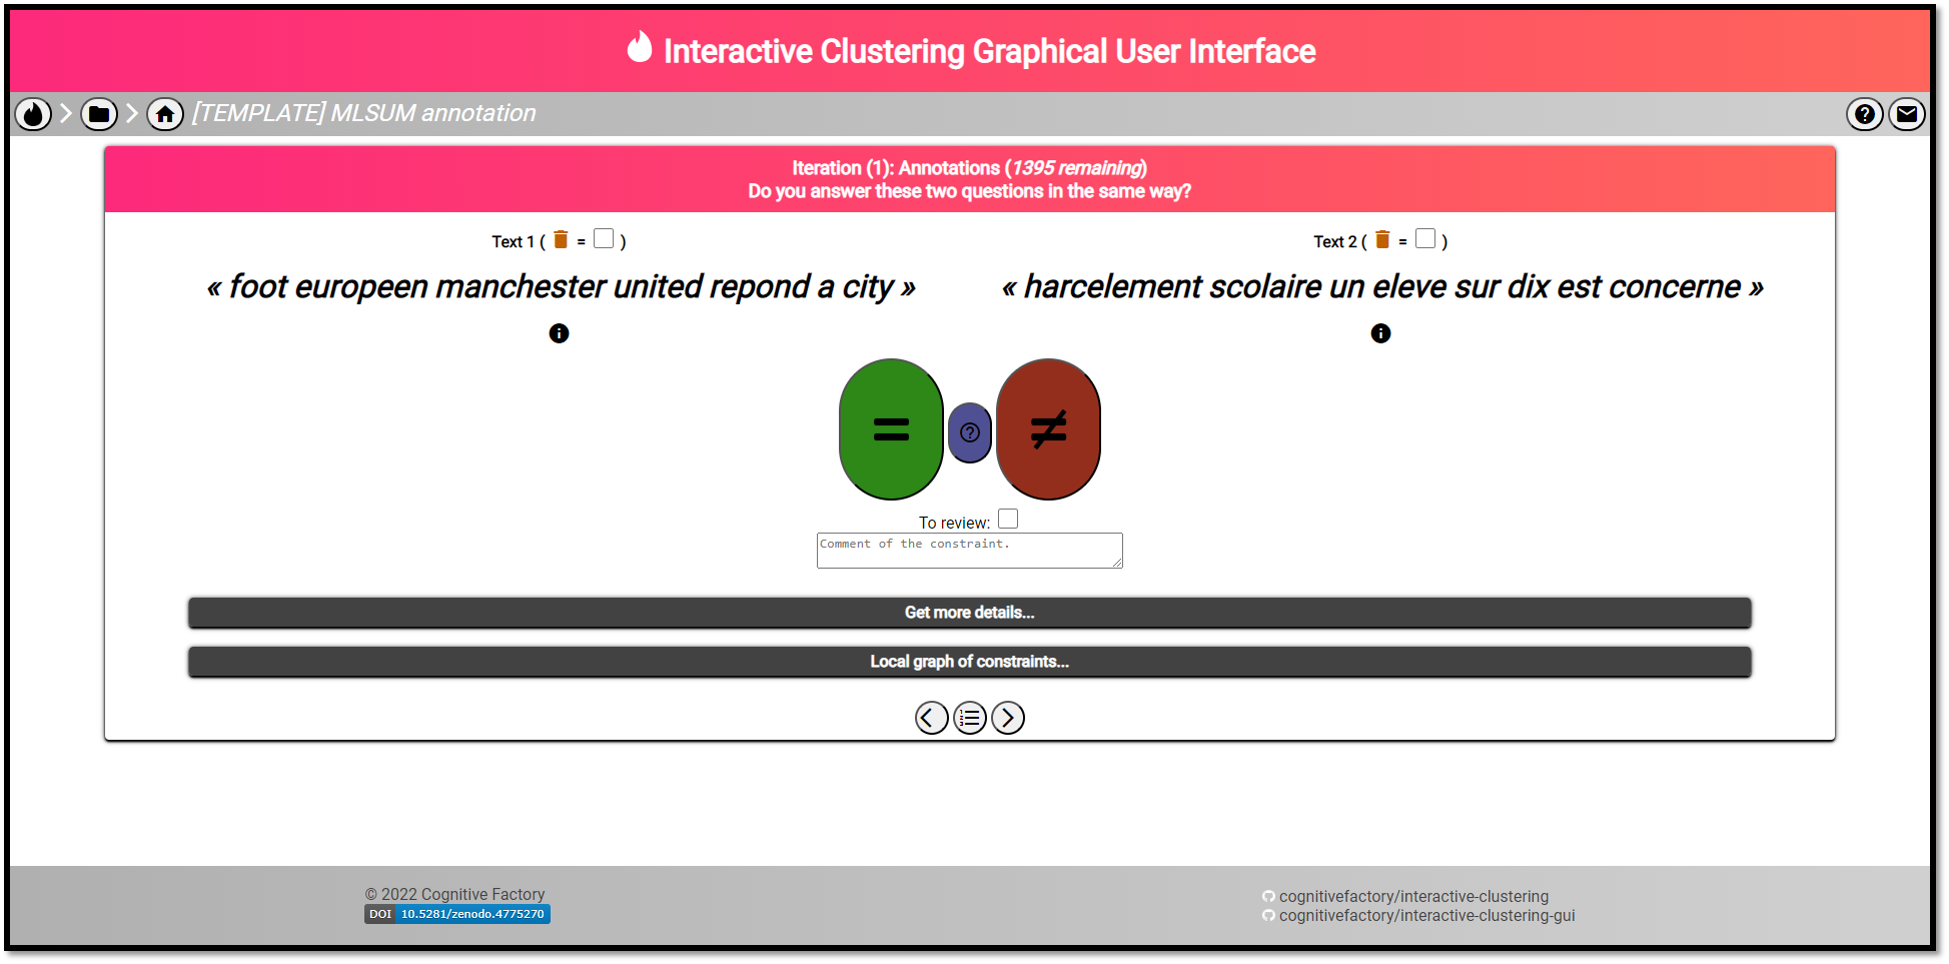
\includegraphics[width=0.95\textwidth]{figures/etude-temps-annotation-0application-annotation}
				\caption{
					Capture d'écran de l'application web permettant d'utiliser notre méthodologie de \texttt{Clustering Interactif} : \textbf{page d'annotation de contraintes}.
					Les deux textes à annoter sont disposés à gauche et à droite de l'écran.
					Chacun dispose d'un case à cocher si le texte n'est pas pertinent à analyser (\textit{ambigu, hors périmètre, incompréhensible, ...}).\\
					Les boutons à disposition permettent respectivement d'annoter un \texttt{MUST-LINK} si les données sont similaires (\textit{bouton \textguillemets{\textcolor{colorApplicationMUSTLINK}{\faEquals}}}), un \texttt{CANNOT-LINK} si les données ne sont pas similaires (\textit{bouton \textguillemets{\textcolor{colorApplicationCANNOTLINK}{\faNotEqual}}}), d'ignorer la contrainte pour laisser la main à l'algorithme de \textit{clustering} (\textit{bouton en bleu}), et d'ajouter un commentaire pour revoir la contrainte plus tard (\textit{case à cocher et champ de texte libre}).
					Deux éléments déroulants permettent d'avoir des informations supplémentaires (\textit{metadata de sélection et de \textit{clustering}, représentation graphique des liens entre contraintes annotées}).
					Les boutons de navigation (\textit{boutons de flèches et de liste}) sont disponibles en bas de page.
				}
				\label{figure:4.3.1-ETUDE-COUTS-TEMPS-ANNOTATION-APPLICATION-ANNOTATION}
			\end{figure}
			\begin{figure}[!htb]
				\centering
				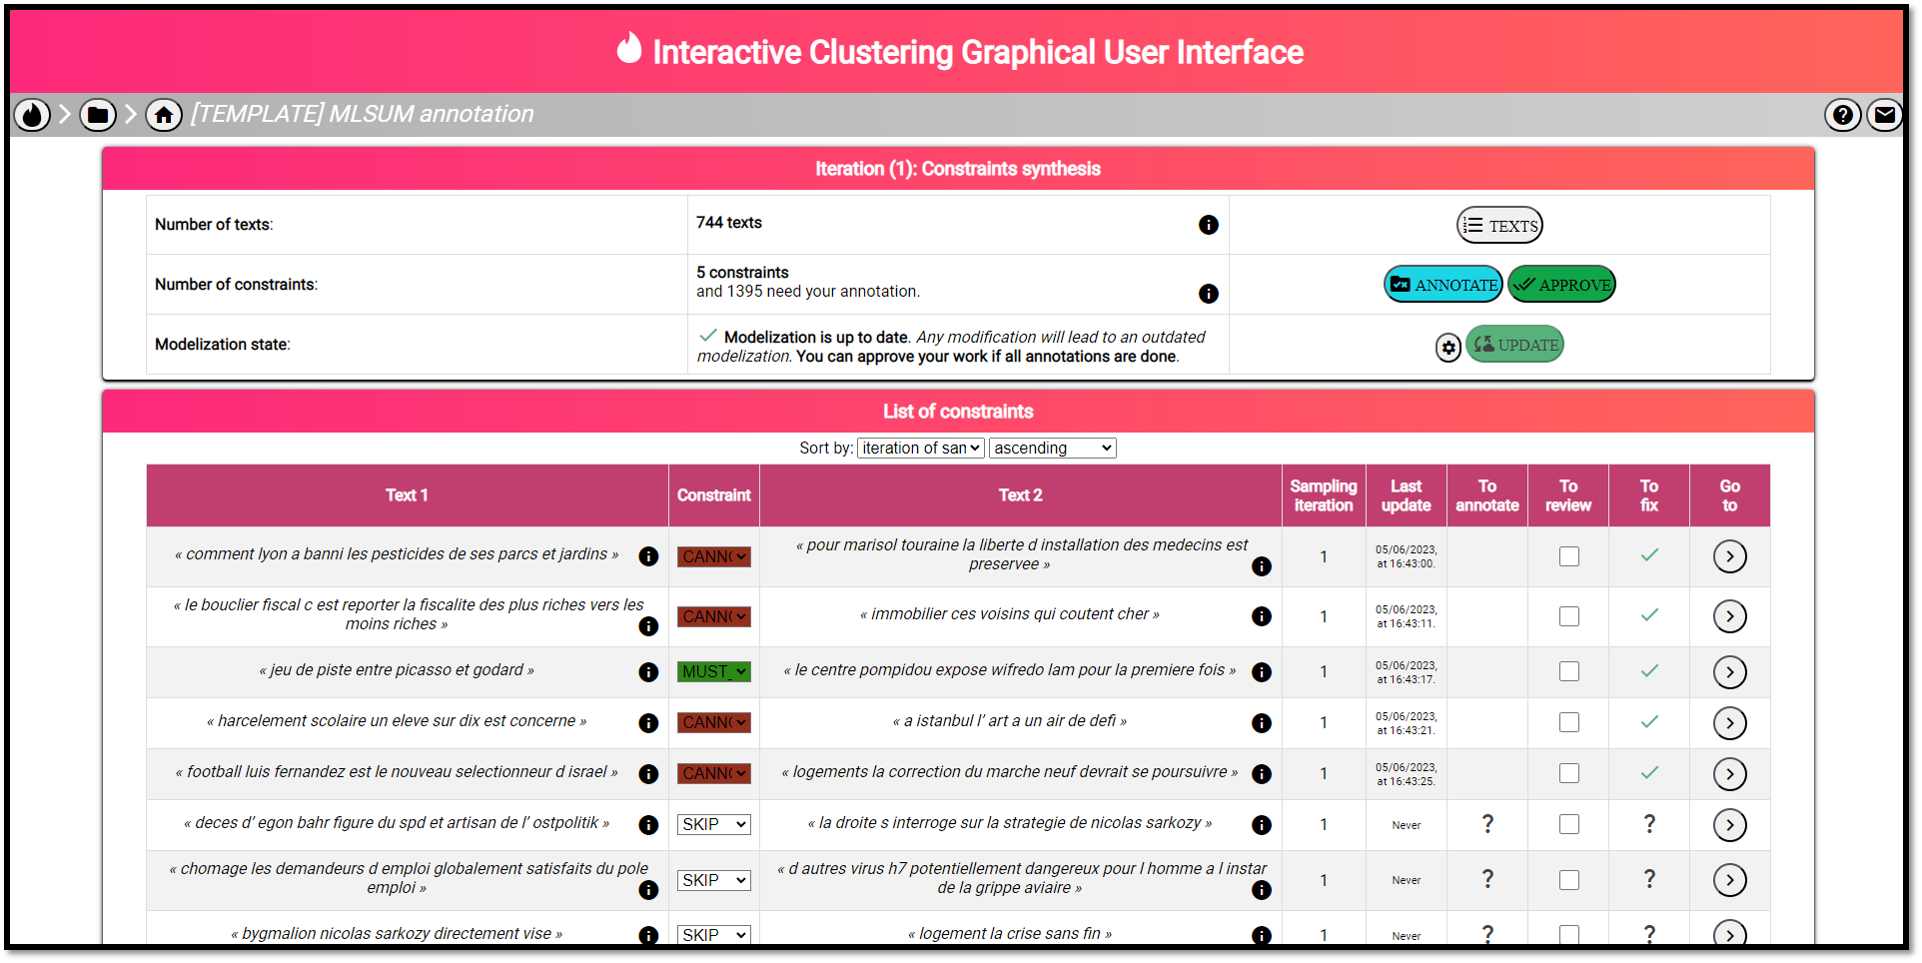
\includegraphics[width=0.95\textwidth]{figures/etude-temps-annotation-0application-liste-contraintes}
				\caption{
					Capture d'écran de l'application web permettant d'utiliser notre méthodologie de \texttt{Clustering Interactif} : \textbf{page d'inventaire des contraintes à annoter}.\\
					La partie supérieure permet d'identifier le nombre de textes et de contraintes sur le projet, ainsi que les boutons destinés à calculer les transitivités entre les contraintes et à approuver le travail réalisé si aucune transitivité n'entre en conflit avec une contrainte annotée.
					La partie inférieure liste l'ensemble des contraintes du projet, avec les annotations réalisées, l'itération à laquelle la contraintes a été sélectionnée et annotée, si elle est à revoir ou si une incohérence la concernant est détectée.
				}
				\label{figure:4.3.1-ETUDE-COUTS-TEMPS-ANNOTATION-APPLICATION-LISTE-CONTRAINTES}
			\end{figure}
			
			
			% Détails de l'expérience : modélisation.
			Une fois les sessions d'annotations terminées, nous entraînons un modèle linéaire généralisé (\textit{GLM}) pour estimer le temps d'annotation moyen pour un lot de contraintes (dont la taille est notée $\texttt{batch\_size}$).
			Ce modèle sera caractérisé par le coefficient de détermination généralisé \texttt{R²} de \textit{Cox et Snel} (\cite{diamond-etal:1990:analysis-binary-data}), la log-vraisemblance \texttt{llf} (\cite{edwards:1992:likelihood}) et la log-vraisemblance \texttt{llf\_null} du modèle \textit{null}.
			Nous discutons aussi de l'évolution de la vitesse d'un opérateur au cours des différentes sessions d'annotation.

			% Référence scripts.
			\setcounter{localCounterOfFootnoteValue}{\value{footnote}}
			\begin{leftBarInformation}
				L'outil d'annotation utilisé est accessible dans \cite{schild-etal:2022:cognitivefactory-interactiveclusteringgui}.
				Les scripts de l'expérience, réalisés avec des \textit{notebooks} \texttt{Python} (\cite{van-rossum-drake:2009:python-reference-manual}), ainsi que le projet à importer dans l'outil d'annotation, sont disponibles dans un dossier dédié de \cite{schild:2021:cognitivefactory-interactiveclusteringcomparativestudy}.
				Nous y utilisons entre autres les librairies \texttt{datetime} \footnotemark et \texttt{statsmodels} \footnotemark (\cite{seabold-perktold:2010:statsmodels-econometric-statistical}).
				De plus, les jeux de données ainsi que les implémentations de notre \texttt{Clustering Interactif} sont détaillés respectivement en \textsc{Annexe~\ref{annex:A-ANNEXE-DATASET}} et en \textsc{Annexe~\ref{annex:C-ANNEXE-IMPLEMENTATIONS}}.
			\end{leftBarInformation}
			%%% Rattraper les footnote.
				\stepcounter{localCounterOfFootnoteValue}
				\footnotetext[\value{localCounterOfFootnoteValue}]{
					\url{https://pypi.org/project/datetime/}
				}
				\stepcounter{localCounterOfFootnoteValue}
				\footnotetext[\value{localCounterOfFootnoteValue}]{
					\url{https://pypi.org/project/statsmodels/}
				}
				

		%%% Résultats.
		\subsubsection{Résultats obtenus}
		
			% Taux de participation.
			Durant cette expérience, $14$ annotateurs ont participé à l'annotation de $1~000$ contraintes aléatoires sur un jeu de données.
			Ces opérateurs travaillent tous dans un service informatique dédié à l'entraînement et l'amélioration de solutions de \textit{Machine Learning} et sont répartis de la manière suivante :
			\begin{itemize}
				\item $4$ femmes, $10$ hommes ;
				\item $7$ personnes entre $20$ et $30$ ans, $7$ personnes entre $30$ et $40$ ans ;
				\item $9$ \textit{Data Scientist}, $4$ développeurs et $1$ ergonome ;
				\item $1$ personne ayant révisé le jeu de données, $3$ le découvrant pour la première fois dont $1$ ayant travaillé auparavant dans le secteur de la presse.
			\end{itemize}
			Par manque de disponibilités, $4$ annotateurs n'ont que partiellement réalisé leur tâche : nous avons toutefois intégré leurs participations car elles contenaient au minimum $150$ annotations.
			
			% Statistiques descriptives.
			D'après les observations, un annotateur réalisait en moyenne $170.7$ contraintes par session d'annotation (min: $43$, max: $547$, médiane: $138$, écart-type: $106.4$) ce qui lui demandait en moyenne $23.1$ minutes (min: $3.0$, max: $92.0$, écart-type: $14.4$).
			De plus, la vitesse d'annotation moyenne était de $7.7$ contraintes par minute (min: $3.5$, max: $14.3$, écart-type: $2.9$).
			
			% Modélisation du temps d'annotation.
			Le modèle linéaire généralisé entraîné sur les mesures de temps d'annotations (\texttt{R²}: $0.910$, \texttt{llf}: $-499.15$, \texttt{llf\_null}: $-539.95$) nous permet de déduire l'équation suivante :
			%
			\begin{equation}
				\label{equation:4.3.1-ETUDE-COUT-COUTS-TEMPS-ANNOTATION}
				\texttt{annotation\_time}~[s]~
				\propto~7.8 \cdot \texttt{batch\_size}
			\end{equation}
		
			% Affichage du temps d'annotation.
			La \textsc{Figure~\ref{figure:4.3.1-ETUDE-COUTS-TEMPS-ANNOTATION-SIMULATION}} représente cette modélisation du temps d'annotation en comparaison avec les mesures réalisées lors de l'expérience.
			Pour rappel, le temps théorique estimé précédemment est de $7$ secondes par contrainte.
			%
			\begin{figure}[!htb]
				\centering
				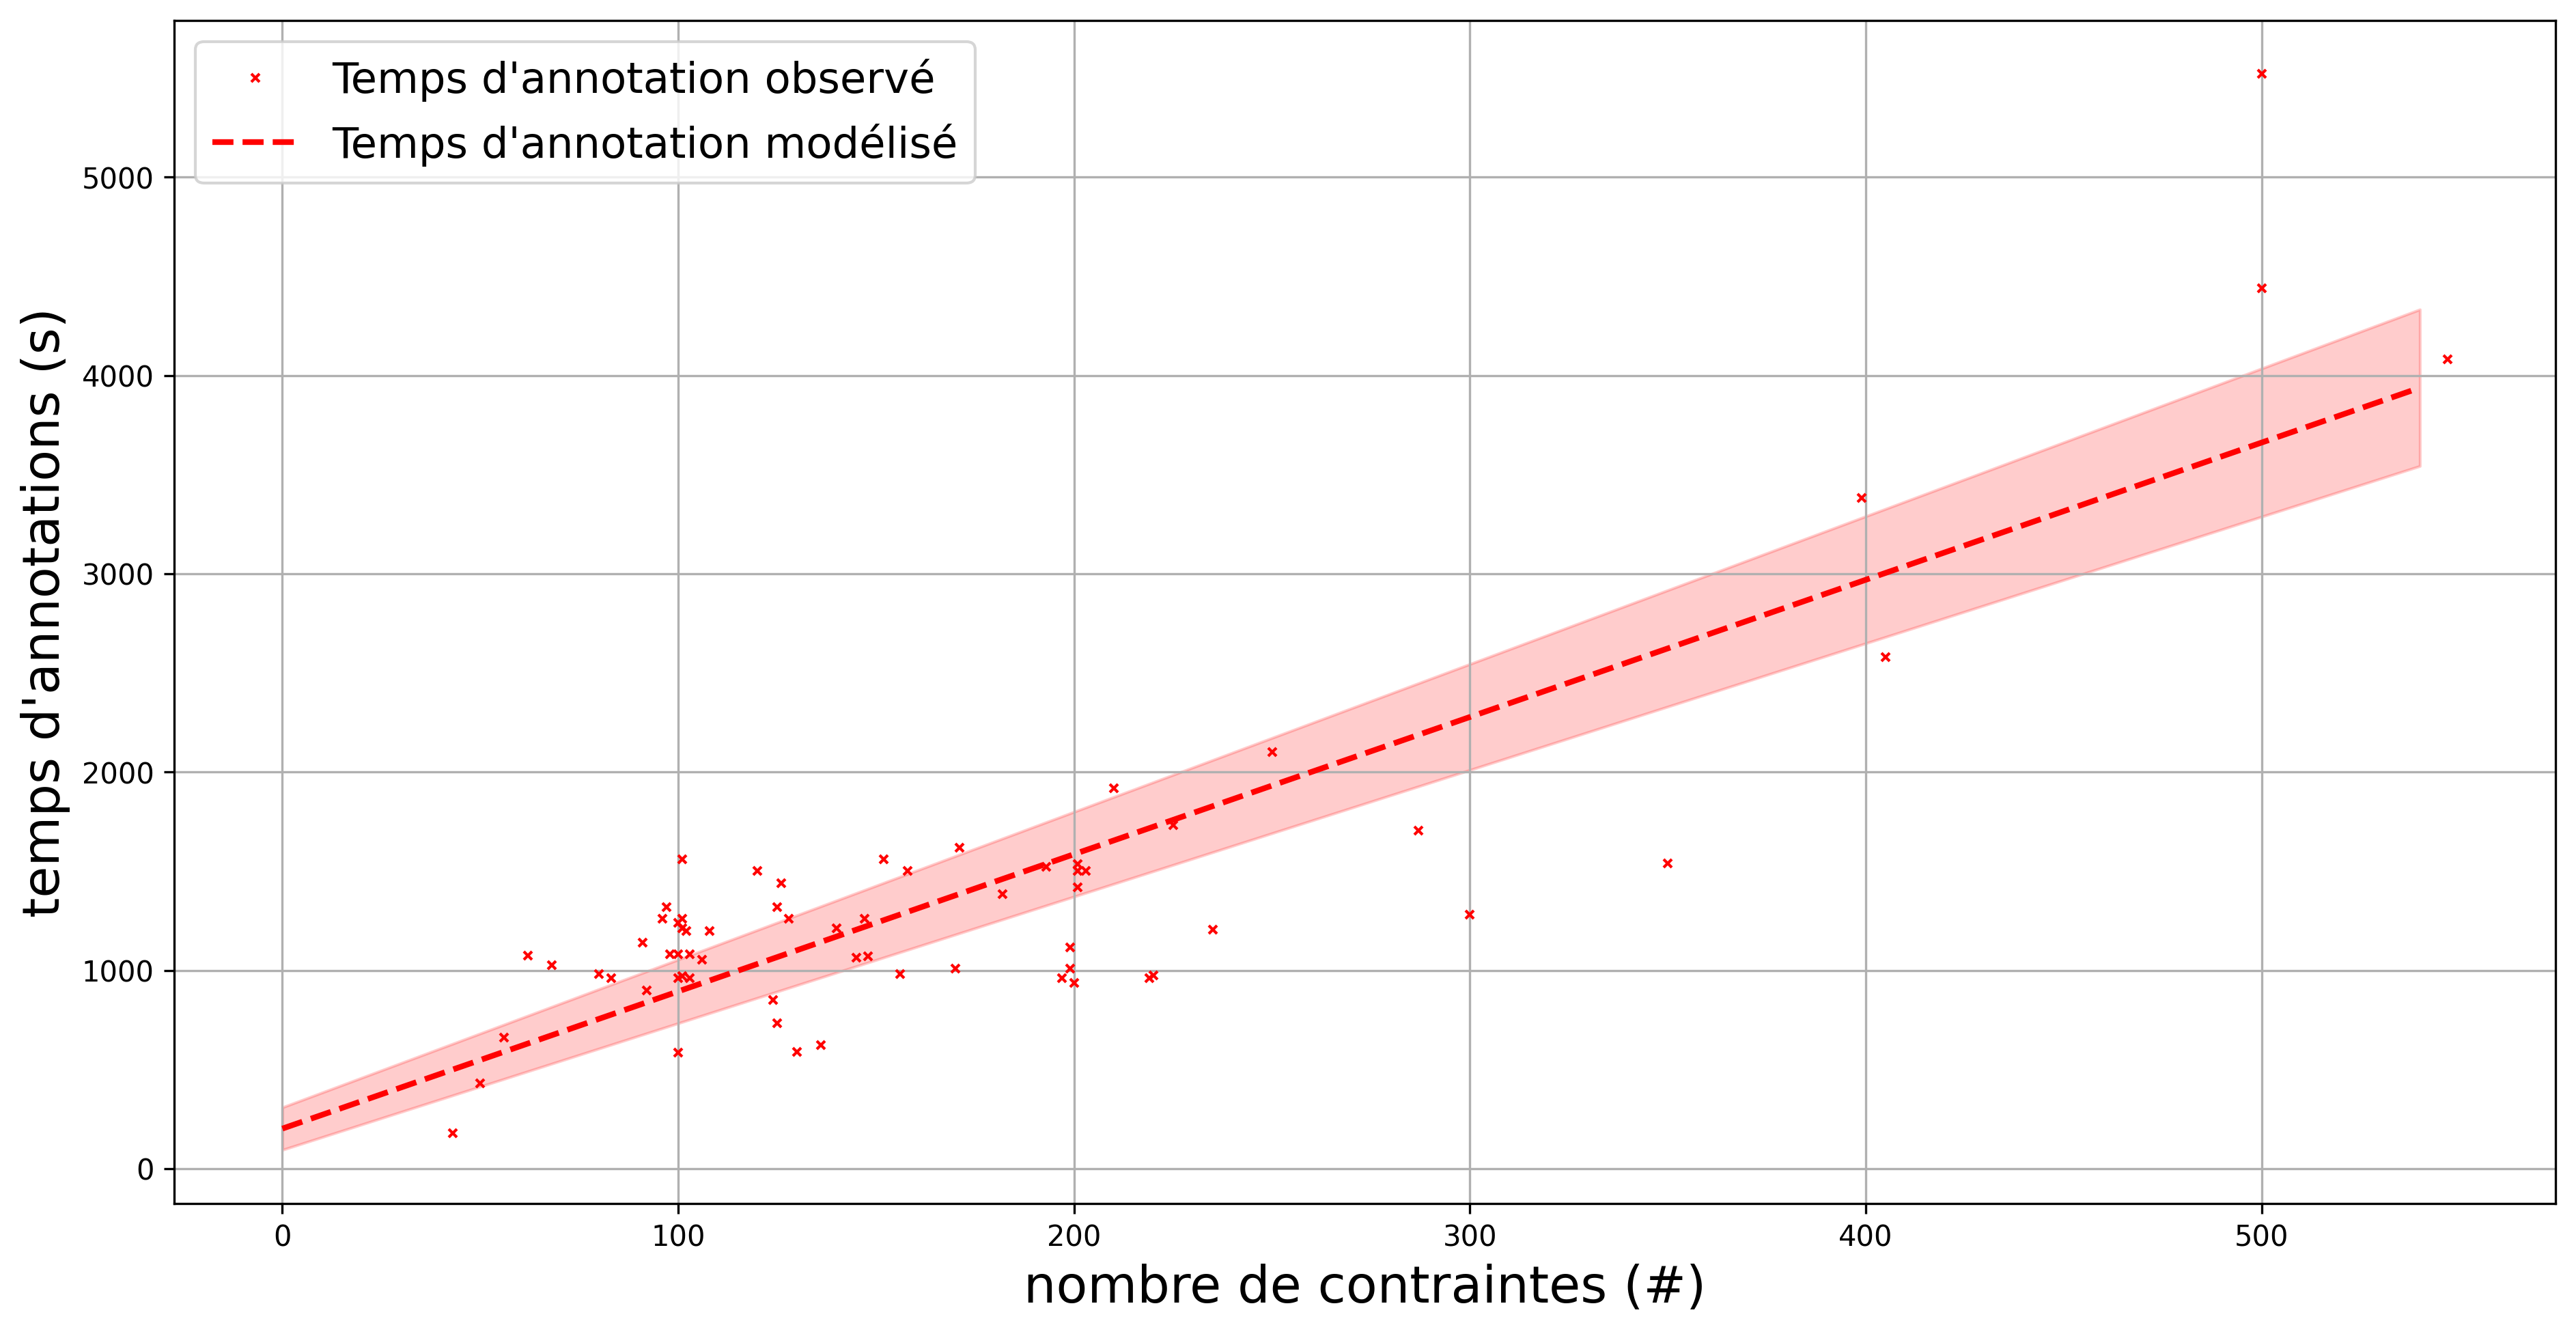
\includegraphics[width=0.95\textwidth]{figures/etude-temps-annotation-1-modelisation-temps}
				\caption{
					Estimation du temps nécessaire (en minutes) pour annoter un lot de contraintes.
				}
				\label{figure:4.3.1-ETUDE-COUTS-TEMPS-ANNOTATION-SIMULATION}
			\end{figure}
		
			% Étude de cas.
			En ce qui concerne l'évolution de la vitesse d'annotation au cours des sessions, aucune tendance significative n'a été identifiée. 
			La \textsc{Figure~\ref{figure:4.3.1-ETUDE-COUTS-TEMPS-ANNOTATION-EXEMPLE}} représente l'évolution de vitesse d'annotation pour quatre opérateurs (les deux plus rapides et les deux plus lents).
			Ces données sont l'objet d'une étude de cas dans la discussion ci-dessous.
			%
			\begin{figure}[!htb]
				\centering
				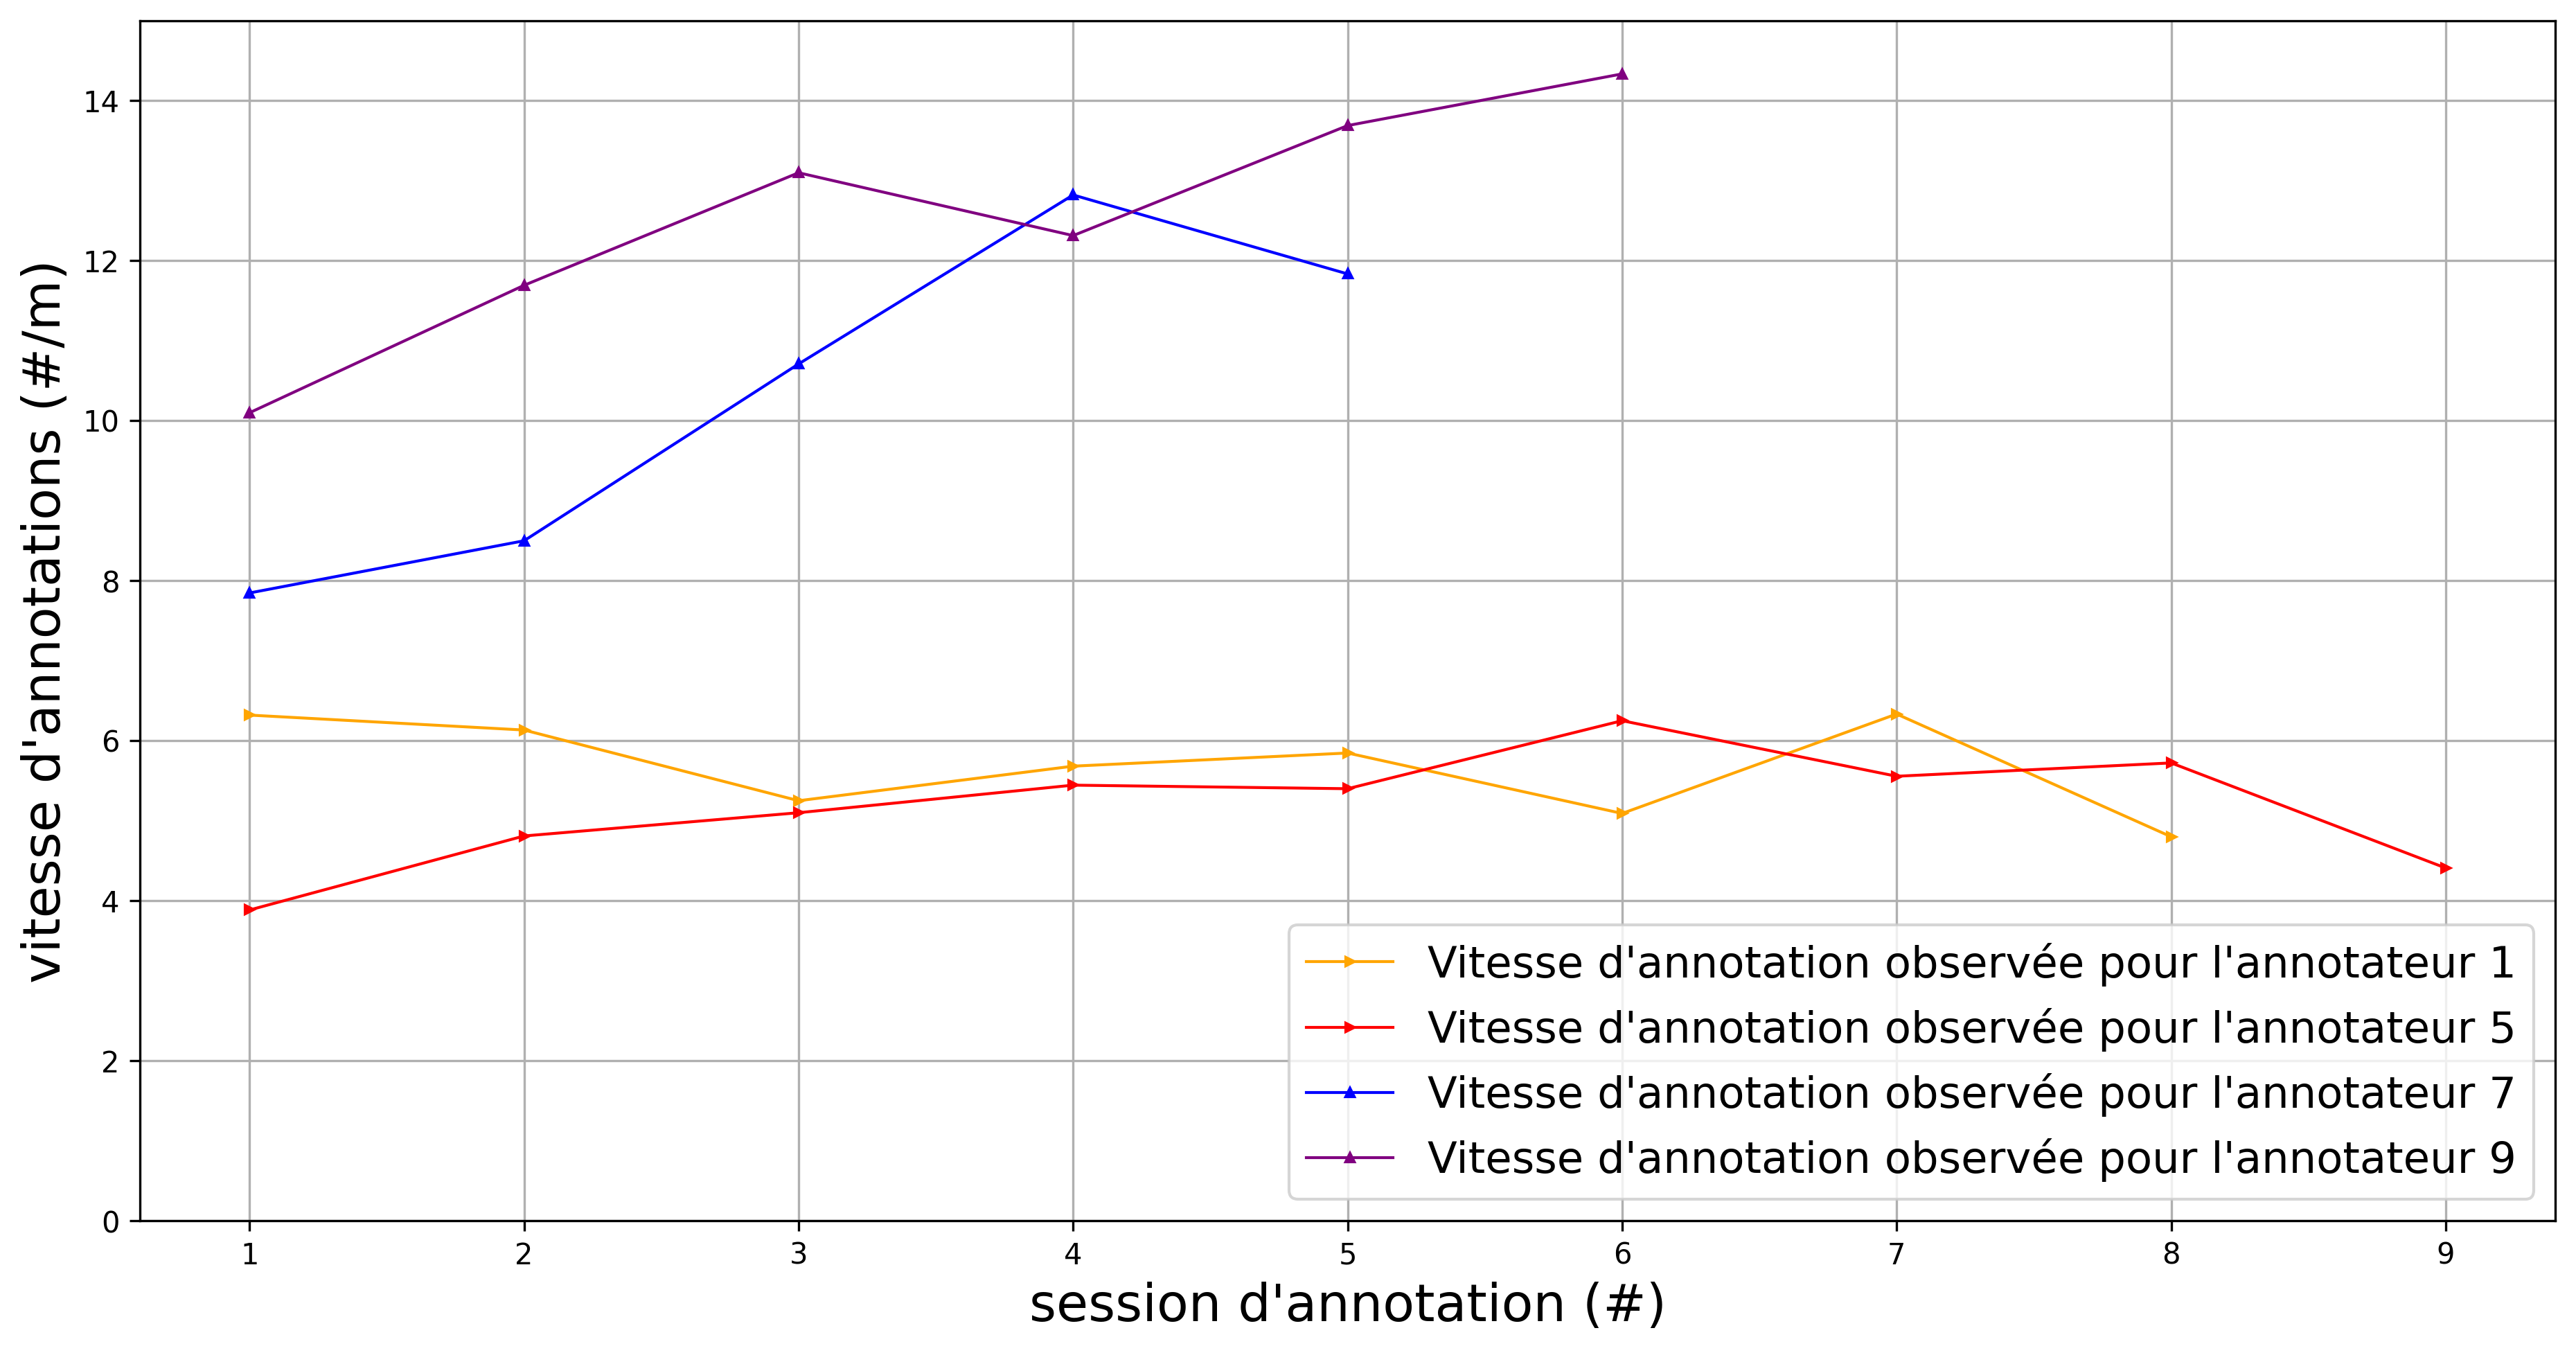
\includegraphics[width=0.95\textwidth]{figures/etude-temps-annotation-3-etude-de-cas}
				\caption{
					Étude de cas d'évolution de la vitesse d'annotation de contraintes (en contraintes par minutes) en fonction des différentes sessions d'annotations.
				}
				\label{figure:4.3.1-ETUDE-COUTS-TEMPS-ANNOTATION-EXEMPLE}
			\end{figure}

		%%% Discussion.
		\subsubsection{Discussion}

		
		% Généralités sur la modélisation du temps d'annotation sur une session.
		L'étude réalisée avec $14$ annotateurs sur des lots de $1~000$ contraintes a permis d'estimer à $7.8 \cdot \texttt{batch\_size}$ le temps nécessaire (en secondes) pour annoter un lot de contraintes (cf. \textsc{Figure~\ref{figure:4.3.1-ETUDE-COUTS-TEMPS-ANNOTATION-SIMULATION}}).
		
		% Compliqué de comparer ...
		\begin{leftBarAuthorOpinion}
			Avant poursuivre la discussion, il est nécessaire de préciser qu'il est difficile de comparer ces résultats.
			% Forte disparité des mesures.
			D'une part, il y a une forte disparité des mesures, et il est idyllique de penser qu'une étude sur $14$ annotateurs peut représenter la diversité du comportement humain sur une tâche aussi complexe que l'annotation de données textuelles.
			% Peu de repères concrets.
			D'autre part, il y a un manque de repères concrets dans la littérature scientifique, entre autres à cause des nombreux facteurs intervenant dans une tâche d'annotation (\textit{objectifs à réaliser, données à manipuler, nombre de choix proposés à l'opérateur, complexité sémantique des données, des compétences de l'opérateur, fréquence d'exécution de la tâche, ...}), mais aussi en raison du manque d'intérêt à l'analyse du temps nécessaire au profit de l'analyse de la cohérence et de la qualité intra- ou inter-annotateur (\cite{baledent:2022:complexite-annotation-manuelle}).
			% Diversité des données.
			De plus, les résultats peuvent différer en fonction des contraintes à caractériser : nous pouvons supposer que des paires de données très similaires ou très différentes sont simples à annoter, mais que des données plus ambiguës peuvent nécessiter davantage de temps pour être intégrées et étiquetées.
			
			% Angle d'attaque.
			Pour pallier ce problème, nous proposons de confronter nos estimations à des mesures réalisées sur des tâches n'ayant pas le même objectif mais dont la complexité est comparable.
			Cette approche, bien qu'un peu rudimentaire, nous permettra ainsi de discuter des ordres de grandeur à manipuler.
		\end{leftBarAuthorOpinion}
		
		
		%%% A. Analyse de l'annotation d'une contrainte.
		\paragraph{Analyse de l'annotation d'une contrainte.}
		
			% Avantage 1: 8 secondes, c'est acceptable.
			En premier lieu, nous voulions confirmer que l'annotation de contraintes est une tâche intuitive dont la durée est caractéristique d'un mécanisme de réaction et non d'une réflexion.
			Pour ce faire, nous avons estimé la durée théorique d'une annotation à $7$ secondes par contrainte, comprenant les temps de lecture, d'analyse de la similitude et d'action de l'opérateur, et nous avons mesuré la durée d'annotation réelle à $7.8$ secondes par contrainte.
			Bien que l'écart constaté ($0.8$ seconde) soit compris dans les bornes d'approximation, cette différence n'est pas suffisamment insignifiante pour nous permettre d'exclure avec certitude la présence d'un mécanisme cognitif supplémentaire.
				
			% Avantage 2: Dans tous les cas, 8 secondes, c'est mieux que 17 secondes ou 40 secondes.
			Pour nous permettre de discuter du temps d'annotation mesuré et de son approximation théorique, nous utilisons utiliser plusieurs points de référence extraits de (\cite{snow-etal:2008:cheap-fast-it}).
			Dans cette étude, les auteurs délèguent quelques tâches d'annotation à \texttt{Amazon Mechanical Turk} \footnote{
				\texttt{Amazon Mechanical Turk} est une plateforme de travail collaboratif en ligne (\textit{crowdsourcing}) : nous avions évoqué leurs fonctionnements, leurs avantages et leurs inconvénients en \textsc{Section~\ref{section:2.3.2.C-DEFIS-ANNOTATION-ASPECT-COMPLEXITE-COUTS}}, notamment le risque de l'abandon de la qualité des annotations au profit de la quantité.
			} :
			
			\begin{enumerate}
				% Task 1: (Word Sense Disambiguation)
				\item Tâche de "\textit{désambiguïsation du sens des mots}" (\cite{pradhan-etal:2007:semeval2007-task-17}).
				Elle consiste à catégoriser le contexte de phrases comportant le mot "\textit{président}" suivant $3$ options préformatées (\textit{dirigeant d'une entreprise, dirigeant des États Unis, dirigeant d'un autre pays}).
				Il y a $177$ phrases à labelliser par $10$ annotateurs, et la tâche a été réalisée en un total de $8.59$ heures, soit une moyenne de $17.5$ secondes par annotation.
				Nous utilisons ce point de repère car la tâche s'apparente à une annotation d'une tâche de classification ($3$ catégories).
				% Task 2: (Word Similarity)
				\item Tâche de "\textit{caractérisation de similitude des mots}" (\cite{miller-charles:1991:contextual-correlates-semantic}).
				Elle consiste à ordonner des paires de mots du plus similaire au moins similaire en fonction de leur proximité sémantique afin de mettre en avant les meilleurs paires de synonymes.
				Il y a $30$ paires de synonymes à ordonner par $10$ annotateurs, et la tâche a été réalisée en un total de $0.17$ heures, soit une moyenne de $2.0$ secondes par annotation.
				Nous utilisons ce point de repère car la tâche s'apparente à l'annotation de contraintes (\textit{laquelle de ces deux paires est la plus adéquate ?}) qui ne fait pas appel à un mécanisme de réflexion (\textit{peu de vocabulaire, similarité intrinsèque triviale entre deux mots}).
				% Task 3: (Recognizing Textual Entailment)
				\item Tâche de "\textit{reconnaissance de l'implication textuelle}" (\cite{dagan-etal:2005:pascal-recognising-textual}).
				Elle consiste à confirmer ou infirmer si une phrase est la conséquence d'une autre (\textit{l'annotation est donc binaire}).
				Il y a $800$ paires de phrases à valider par $10$ annotateurs, et la tâche a été réalisée en un total de $89.3$ heures, soit une moyenne de $40.2$ secondes par annotation.
				Nous utilisons ce point de repère car la tâche s'apparente à l'annotation de contraintes (\textit{est-ce que l'implication est vraie ?}) faisant intervenir un mécanisme de réflexion (\textit{comprendre une implication logique}).
			\end{enumerate}
			%
			% Comparaison à Task 1: (Word Sense Disambiguation).
			En utilisant la tâche de "\textit{désambiguïsation du sens des mots}" (1.), nous avons déjà un point de comparaison entre notre annotation de contraintes et une annotation classique de classes.
			Nous constatons une nette différence entre les deux approches ($7.8$ secondes par contrainte vs $17.5$ secondes par donnée), cela met en avant qu'une annotation de contraintes est plus rapide qu'une annotation par label.
			
			% Comparaison à Task 2: (Word Similarity).
			Ensuite, en utilisant la tâche de "\textit{caractérisation de similitude des mots}" (2.), nous pouvons confirmer que notre approximation théorique (faisant intervenir un traitement cognitif de $1$ seconde) semble adaptée pour représenter un mécanisme de l'ordre de la réaction.
			En effet, le coût très faible de la caractérisation d'une similarité entre deux mots ($2.0$ secondes par paire de mots) s'avère être en adéquation avec cette approximation ($2.5$ secondes par paire de phrases de taille $1$).
			
			% Comparaison à Task 3: (Recognizing Textual Entailment).
			Enfin, en utilisant la tâche de "\textit{reconnaissance de l'implication textuelle}" (3.), nous comparons deux annotations binaires dont une fait nettement appel à un mécanisme de réflexion (déduction logique dans une implication).
			Nous constatons une très nette différence entre les deux approches ($7.8$ secondes par contrainte vs $40.2$ secondes par implication), ce qui nous permet d'exclure la présence de mécanisme cognitif trop complexe.
	
			% Conclusion sur l'analyse de l'annotation d'une contraintes.
			\begin{leftBarSummary}
				Mettant bout à bout ces comparaisons, et en gardant à l'esprit que ces références restent approximatives, nous pouvons conclure que (1) \textbf{l'annotation de contraintes est une tâche plus rapide qu'une annotation par label} et que (2) \textbf{cette annotation binaire ne semble pas faire pas intervenir de traitement cognitif complexe} (\textit{c'est une piste à explorer plus en détails pour expliquer le gain de temps observé}).
			\end{leftBarSummary}
		
		
		%%% B. Analyse d'une session d'annotation de contraintes.
		\paragraph{Analyse d'une session d'annotation de contraintes.}
		
			% Ouverture 1: Autres analyses sans conclusions.
			Nous avons analysé l'évolution de la vitesse d'annotation au cours des sessions d'annotation, en espérant observer une accélération des annotations au fur et à mesure que l'annotateur s'habitue avec la tâche, ainsi qu'un effet de fatigue pour des sessions d'annotations trop longues.
			Cependant, aucune de nos analyses n'a montré de résultats significatifs (on peut constater la forte dispersion des résultats grâce à la \textsc{Figure~\ref{figure:4.3.1-ETUDE-COUTS-TEMPS-ANNOTATION-EXEMPLE}}).
			Nous ne pouvons donc pas conclure sur de telles tendances.
			
			\begin{leftBarAuthorOpinion}
				Nos intuitions initiales concernaient deux points :
				\begin{itemize}
					% Temps d'adaptation.
					\item la diminution du \textbf{temps d'adaptation} au cours de sessions d'annotations : au fur et à mesure qu'il annote, l'opérateur pourrait entrer plus facilement dans sa tâche, lui permettant d'atteindre plus rapidement sa vitesse de croisière et ainsi gagner en efficacité sur plusieurs sessions.
					D'après \cite{anderson:2013:architecture-cognition}, ce temps d'adaptation pourrait se définir en trois étapes : une phase déclarative (\textit{besoin d'instructions détaillées, exécution lente et avec erreurs}), une phase associative (\textit{quelques rappels clés suffisent pour retrouver les instructions, donc gain de vitesse}) et une phase autonome (\textit{les consignes sont acquises, donc exécution rapide et sans erreur}) ;
					% Effet de fatigue.
					\item l'intervention d'un \textbf{effet de fatigue} : si une session d'annotation dure trop longtemps, l'opérateur pourrait perdre en efficacité par manque de concentration et augmenter ses chances de faire des erreurs.
					D'après \cite{jones-etal:2015:demographic-occupational-predictors}, la fatigue est considérée comme un inconfort qui s'installe après une tâche excessive, et \cite{elkosantini-gien:2009:integration-human-behavioural} décrit cet état de fatigue par des capacités de travail réduites.
				\end{itemize}
				%
				Ces différentes intuitions ont aussi été remontées par les annotateurs de notre expérience, mais aucun effet significatif n'a pu être observé.
			\end{leftBarAuthorOpinion}
		
			% Ouverture 2: Remarque sur le nombre maximal moyen de contraintes à annoter.
			Par extension, nous ne pouvons pas non plus conclure sur la taille optimale d'échantillon de contraintes à sélectionner pour une session d'annotation.
			Dans nos précédentes études, nous avions arbitrairement fixé la taille de lot à $50$ pour bénéficier d'itérations brèves, permettant à l'algorithme de \textit{clustering} de s'améliorer régulièrement avec les dernières contraintes.
			Mais des petits lots d'annotation démultiplient le nombre d'itérations à réaliser, et donc le nombre d'algorithmes à exécuter.
			Il serait donc judicieux d'adapter le nombre d'annotations à réaliser pour améliorer l'expérience utilisateur en situation réelle de l'opérateur.
			Malheureusement, aucun repère significatif ne peut être déduit de nos résultats pour prédire la fin d'un temps d'adaptation ou le début d'un effet de fatigue.
			
			% Idées : nombre de contraintes moyen par session.
			Afin de proposer tout de même un ordre de grandeur de taille de lot, nous pouvons nous intéresser au nombre moyen de contraintes annotées lors des sessions réalisées par les opérateurs de notre expérience.
			Bien que ces informations n'aient pas été collectées initialement à cette fin, nous pouvons supposer que les opérateurs ont interrompu leur session pour se reposer (\textit{par fatigue, ennui, agacement, ...}) ou répondre à une autre sollicitation (\textit{intervention d'un collègue, mail important, pause café, ...})
			Après un entretien avec les opérateurs de notre expérience, il semble y avoir deux possibilités : soit l'opérateur ne se fixait pas d'objectif et s'arrêtait par fatigue ; soit il se fixait un objectif (\textit{de nombre ou de durée}), mais adaptait son prochain objectif en fonction de la fatigue ressentie en fin de session.
			Dans les deux cas, nous pouvons faire l'hypothèse que le nombre moyen d'annotation par session tend à représenter une borne supérieure de la taille maximale d'un lot à considérer pour ne pas entamer l'effet de fatigue.
			Sur l'expérience réalisée, cette moyenne est de $170.70$ contraintes annotées par session (écart-type: $106.37$, erreur standard: $13.19$).
			En prenant en compte une marge d'erreur pour minimiser ce résultat, nous retenons $150$ contraintes comme seuil à ne pas dépasser.
			
			% Conclusion sur l'analyse d'une session d'annotation de contraintes.
			\begin{leftBarSummary}
				Pour une session d'annotation, \textbf{nous conseillons une taille d'échantillon entre $50$ et $150$ contraintes}.
				Attention aux échantillons trop petits qui multiplient le nombre d'itérations à réaliser ;
				Attention aussi aux échantillons trop gros qui peuvent introduire un effet de fatigue chez l'opérateur et casser la dynamique d'interactions avec la machine.
				La discussion finale de ce chapitre affinera cette fourchette grâce à une vue d'ensemble sur les coûts de la méthode.
			\end{leftBarSummary}
			

		%%% C. Analyse des fonctionnalités de l'application d'annotation
		\paragraph{Analyse des fonctionnalités de l'application d'annotation.}
		
			% Ouverture 3: Autres remontées applicatives.
			Pour finir cette discussion, nous nous intéressons à l'utilisation du logiciel par nos opérateurs au cours de cette étude.
			En effet, il est logique de penser que la conception de l'application et les fonctionnalités dont elle dispose peut grandement impacter l'expérience utilisateur de notre méthodologie de \textit{clustering} itératif.
			Un entretien avec les opérateurs a permis de remonter plusieurs pistes d'amélioration de son ergonomie.
			
			% Idées 1: Données non prétraitées.
			Un premier point concerne l'affichage des textes d'une contrainte.
			Comme montré en \textsc{Figure~\ref{figure:4.3.1-ETUDE-COUTS-TEMPS-ANNOTATION-APPLICATION-ANNOTATION}}, nous avions choisi d'afficher des données normalisées à l'écran pour masquer le bruit provoqué par les accents, les majuscules, la ponctuation.
			Bien que cette fonctionnalité peut servir pour des textes bruts (\textit{issus de conversations clients ou de forums par exemple}), cela a plutôt nuit à la compréhension des données par les opérateurs.
			Nous avons donc envisagé de laisser la données brutes à disposition, dans une infobulle ou grâce à une option permettant d'interchanger le format des données.
			
			% Idée 2: Ordonner les données.
			Une seconde proposition concerne l'ordre des contraintes à annoter.
			Nous pouvons facilement admettre que la compréhension rapide d'un grand nombre de textes est une tâche pénible.
			Pour soulager les opérateurs et limiter le nombre de changement de contexte, nous avons trié les contraintes par ordre alphabétique.
			Ainsi, toutes les contraintes associées à une même donnée peuvent être traitées à la suite.
			Cette solution peut faciliter la caractérisation d'une similitude en analysant à la chaîne plusieurs données du même type.
			À cet effet, une option de tri à été ajoutée sur la liste de contraintes à traiter (cf. \textsc{Figure~\ref{figure:4.3.1-ETUDE-COUTS-TEMPS-ANNOTATION-APPLICATION-LISTE-CONTRAINTES}}).
			
			% Idée 3: Annotation multi-contraintes.
			Enfin, une dernière idée concerne l'affichage des données à annoter.
			Nous avions jusqu'à présent considéré l'annotation entre deux données (cf. \textsc{Figure~\ref{figure:4.3.1-ETUDE-COUTS-TEMPS-ANNOTATION-APPLICATION-ANNOTATION}}), mais il peut être judicieux d'afficher plusieurs données à caractériser simultanément.
			Une telle fonctionnalité permettrait ainsi de regrouper rapidement un grand nombre de données similaires ou de distinguer avec moins d'ambiguïté certaines données en s'appuyant sur leur voisinage.
			
			\begin{leftBarInformation}
				Ces différentes évolutions sont en cours d'analyse ou ont déjà été intégrées dans l'application que nous proposons (\cite{schild-etal:2022:cognitivefactory-interactiveclusteringgui}).
			\end{leftBarInformation}
	

	%%%
	%%% Subsection 4.3.2: Étude du temps de calcul nécessaire aux algorithmes implémentés en chronométrant des exécutions dans différentes situations
	%%%
	\subsection{Étude du temps de calcul nécessaire aux algorithmes implémentés en chronométrant des exécutions dans différentes situations}
	\label{section:4.3.2-ETUDE-COUTS-TEMPS-CALCUL}
		
		% Transition.
		Maintenant que nous avons pu modéliser le temps nécessaire à un expert pour annoter un lot de contraintes, nous nous intéressons au temps nécessaire à la machine pour interpréter ces annotations et proposer une nouvelle segmentation des données.
		
		% Complexité de la tâche.
		Comme les différents algorithmes employés manipulent des contraintes sur les données, l'estimation théorique du temps d'exécution par l'analyse de la complexité ne semble pas fiable : en effet, quelques contraintes bien placées peuvent suffire à simplifier le fonctionnement d'un algorithme de \textit{clustering} alors qu'une grande quantité de contraintes mal placées vont au contraire le pénaliser.
		% Objectif de l'expérience.
		Nous préférons donc une approche empirique en chronométrant plusieurs exécutions isolées des algorithmes intervenant dans notre implémentation du \texttt{Clustering Interactif} et en évaluant l'importance de leurs différents arguments d'entrée (la taille du jeu de données, le nombre de \textit{clusters} et le nombre de contraintes annotées, ...).
		Nous profitons aussi de ces modélisations du temps de calcul pour confirmer le choix de paramétrage réalisé lors de l'étude d'efficience en \textsc{Section~\ref{section:4.2-HYPOTHESE-EFFICIENCE}}, et ainsi faire un compromis entre l'algorithme le plus efficient et l'algorithme le plus rapide.
	
		%%% Protocole expérimental.
		\subsubsection{Protocole expérimental}
			
			% Pseudo-code.
			Pour résumer le protocole expérimental que nous détaillons ci-dessous, une description en pseudo-code est disponible dans l'\textsc{Algorithme~\ref{algorithm:4.3.2-ETUDE-COUTS-TEMPS-CALCUL-PROTOCOLE}}.
			
			\begin{algorithm}
				\KwData{jeux de données annotées (vérités terrains) de tailles différentes}
				\KwIn{combinaisons d'algorithmes et de paramètres à tester}
				%
				\ForEach{combinaison d'algorithmes et de paramètres à tester}{
					\textbf{initialisation (données)}: récupérer ou générer le jeu de données \;
					\textbf{initialisation (contraintes)}: créer une liste vide de contraintes \;
					\If{estimation de la tâche de \textbf{prétraitements}}{
						\textbf{chronomètre}: \textbf{START} \;
						\textbf{prétraitements (à étudier)}: supprimer le bruit dans les données \;
						\textbf{chronomètre}: \textbf{STOP} \;
					}
					\ElseIf {estimation de la tâche de \textbf{vectorisation}}{
						\textbf{prétraitements}: supprimer le bruit dans les données avec \texttt{prep.simple} \;
						\textbf{chronomètre}: \textbf{START} \;
						\textbf{vectorisation (à étudier)}: transformer les données en vecteurs \;
						\textbf{chronomètre}: \textbf{STOP} \;
					}
					\ElseIf {estimation de la tâche de \textbf{clustering}}{
						\textbf{prétraitements}: supprimer le bruit dans les données avec \texttt{prep.simple} \;
						\textbf{vectorisation}: transformer les données en vecteurs avec \texttt{vect.tfidf} \;
						\textbf{échantillonnage initial}: sélectionner des contraintes avec \texttt{samp.rand.full} \;
						\textbf{simulation d'annotation}: déterminer les contraintes avec la vérité terrain \;
						\textbf{intégration}: ajouter les nouvelles contraintes au gestionnaire de contraintes \;
						\textbf{chronomètre}: \textbf{START} \;
						\textbf{clustering (à étudier)}: regrouper les données par similarité \;
						\textbf{chronomètre}: \textbf{STOP} \;
					}
					\ElseIf {estimation de la tâche d'\textbf{échantillonnage}}{
						\textbf{prétraitements}: supprimer le bruit dans les données avec \texttt{prep.simple} \;
						\textbf{vectorisation}: transformer les données en vecteurs avec \texttt{vect.tfidf} \;
						\textbf{échantillonnage initial}: sélectionner des contraintes avec \texttt{samp.rand.full} \;
						\textbf{simulation d'annotation}: déterminer les contraintes avec la vérité terrain \;
						\textbf{intégration}: ajouter les nouvelles contraintes au gestionnaire de contraintes \;
						\textbf{clustering initial}: regrouper les données avec \texttt{clust.kmeans.cop} \;
						\textbf{chronomètre}: \textbf{START} \;
						\textbf{échantillonnage (à étudier)}: sélectionner de nouvelles contraintes à annoter \;
						\textbf{chronomètre}: \textbf{STOP} \;
					}
				}
				\ForEach{algorithme à modéliser}{
					\textbf{cadrage}: définir les facteurs et les interactions intervenant dans la modélisation \;
					\textbf{simplification}: restreindre la modélisation aux facteurs les plus corrélés \;
					\textbf{analyse}: modéliser le temps d'exécution avec les facteurs retenus \;
				}
				%
				\KwResult{modélisation du temps d'exécution des différents algorithmes}
				%
				\caption{\textit{
					Description en pseudo-code du protocole expérimental de l'étude du temps d'exécution des algorithmes du \texttt{Clustering Interactif}.
				}}
				\label{algorithm:4.3.2-ETUDE-COUTS-TEMPS-CALCUL-PROTOCOLE}
			\end{algorithm}
			
			% Description de la vérité terrain.
			Nous utilisons le jeu de données \texttt{Bank Cards (v2.0.0)} comme référence pour cette expérience : ce dernier traite des demandes les plus fréquentes des clients en ce qui concerne la gestion de leur carte bancaire.
			Il est composé de $1~000$ questions rédigées en français et réparties en $10$ classes (\texttt{perte ou vol de carte}, \texttt{carte avalée}, \texttt{commande de carte}, ...).
			Pour plus de détails, consulter l'\textsc{Annexe~\ref{annex:A.1-DATASET-BANK-CARDS}}.
			Cependant, un seul jeu de données ne nous permet pas d'analyser l'impact du nombre de données sur le temps d'exécution des algorithmes.
			Pour utiliser facilement plusieurs jeux de données de tailles différentes tout en maîtrisant leur contenu, nous avons donc dupliqué aléatoirement des données issues du jeu de référence en y insérant des fautes de frappes.
			
			% Remarques.
			\begin{leftBarWarning}
				Dans le cadre de cette étude, nous faisons l'hypothèse que cette création artificielle de données n'a pas d'impact majeur sur le temps d'exécution des différents algorithmes.
			\end{leftBarWarning}
			
			% Description des tâches, des algorithmes et des contextes.
			À l'aide de ces données, nous lançons plusieurs exécutions de chaque algorithme de notre implémentation du \texttt{Clustering Interactif} avec différentes variations de contexte d'utilisation.
			Cette implémentation est détaillée en \textsc{Annexe~\ref{annex:C.1-DESCRIPTION-IMPLEMENTATION-INTERACTIVE-CLUSTERING}}.
			Cela comprend les tâches, algorithmes et contextes d'utilisation suivants :
			\begin{enumerate}
				% Prétraitement.
				\item le \textbf{prétraitements} des données...
					\begin{itemize}
						\item avec les algorithmes suivants : \textbf{simples} (noté \texttt{prep.simple}), \textbf{avec lemmatisation} (noté \texttt{prep.lemma}) et \textbf{avec filtres} (noté \texttt{prep.filter}) ;
						\item avec les contextes d'utilisation suivants : \textbf{nombre de données} (variant de $1~000$ à $5~000$ par pas de $1~000$, noté $\texttt{dataset\_size}$) ;
					\end{itemize}
				% Vectorisation.
				\item la \textbf{vectorisation} des données...
					\begin{itemize}
						\item avec les algorithmes suivants : \textbf{TF-IDF} (noté \texttt{vect.tfidf}) et \textbf{SpaCy} (noté \texttt{vect.frcorenewsmd}) ;
						\item avec les contextes d'utilisation suivants : \textbf{nombre de données} (variant de $1~000$ à $5~000$ par pas de $1~000$, noté $\texttt{dataset\_size}$) ;
						\item le tout précédé par des prétraitements \textbf{simples} ;
					\end{itemize}
				% \textit{Clustering}.
				\item le \textbf{\textit{clustering} sous contraintes} des données...
					\begin{itemize}
						\item avec les algorithmes suivants : \textbf{KMeans} (modèle \textit{COP} noté \texttt{clust.kmeans.cop}), \textbf{Hiérarchique} (lien \textit{single} noté \texttt{clust.hier.sing} ; lien \textit{complete} noté \texttt{clust.hier.comp} ; lien \textit{average} noté \texttt{clust.hier.avg} ; lien \textit{ward} noté \texttt{clust.hier.ward}) et \textbf{Spectral} (modèle \textit{SPEC} noté \texttt{clust.spec}) ;
						\item avec les contextes d'utilisation suivants : \textbf{nombre de données} (variant de $1~000$ à $5~000$ par pas de $1~000$, noté $\texttt{dataset\_size}$), le \textbf{nombre de contraintes annotées} (variant de $0$ à $5~000$ par pas de $500$, noté $\texttt{previous\_nb\_constraints}$) et le \textbf{nombre de \textit{clusters} à trouver} (variant de $5$ à $50$ par pas de $5$, noté $\texttt{algorithm\_nb\_clusters}$) ;
						\item le tout précédé par des prétraitements \textbf{simples} et une vectorisation \textbf{TF-IDF} et un échantillonnage initial \textbf{purement aléatoire} ;
					\end{itemize}
				% Sampling.
				\item l'\textbf{échantillonnage} des contraintes à annoter...
					\begin{itemize}
						\item avec les algorithmes suivants : \textbf{purement aléatoire} (noté \texttt{samp.random.full}), \textbf{pseudo-aléatoire} (noté \texttt{samp.random.same}), \textbf{même \textit{cluster} mais étant les plus éloignés} (noté \texttt{samp.farthest.same}) et \textbf{\textit{clusters} différents mais étant les plus proches} (noté \texttt{samp.closest.diff}) ;
						\item avec les contextes d'utilisation suivants : \textbf{nombre de données} (variant de $1~000$ à $5~000$ par pas de $1~000$, noté $\texttt{dataset\_size}$), le \textbf{nombre de contraintes annotées} (variant de $0$ à $5~000$ par pas de $500$, noté $\texttt{previous\_nb\_constraints}$), le \textbf{nombre de \textit{\textit{clusters}} existants} (variant de $10$ à $50$ par pas de $10$, noté $\texttt{previous\_nb\_clusters}$) et le \textbf{nombre de contraintes à sélectionner} (variant de $50$ à $250$ par pas de $50$, noté $\texttt{algorithm\_nb\_constraints}$) ;
						\item le tout précédé par des prétraitements \textbf{simples}, une vectorisation \textbf{TF-IDF}, un \textit{clustering} initial \textbf{KMeans} (modèle \textit{COP}) et un échantillonnage initial \textbf{purement aléatoire} ;
					\end{itemize}
			\end{enumerate}
			
			Il y a donc $8~825$ combinaisons d'algorithmes (\texttt{15} pour les prétraitements, $10$ pour la vectorisation, $3~330$ pour le \textit{clustering}, $5~550$ pour l'échantillonnage), et chaque combinaison est répétée $5$ fois pour contrer les aléas statistiques des exécutions.
			De plus, chaque jeu de données est généré $5$ fois pour contrer les aléas statistiques de création, donc il y a $220~625$ exécutions d'algorithmes ($375$ pour les prétraitements, $250$ pour la vectorisation, $82~500$ pour le \textit{clustering}, $137~500$ pour l'échantillonnage).
			
			% Description de la modélisation.
			Sur la base de ces mesures, nous cherchons à modéliser le temps d'exécution de chaque algorithme en fonction de son contexte d'utilisation (dépendant de ses arguments d'entrée), et les interactions doubles entre paramètres sont envisagées.
			Afin de réduire la complexité des modélisations, nous ordonnons les interactions de facteurs possibles en fonction de leur corrélation avec le temps mesuré (la corrélation \texttt{r} de \textit{Pearson} (\cite{kirch:2008:pearson-correlation-coefficient}) est utilisée) et nous nous limitons aux variables responsables d'un maximum de la variance des mesures (la méthode d'\textit{Elbow} (\cite{thorndike:1953:who-belongs-family}) est utilisée pour choisir les facteurs pertinents).
			Sur cette base, nous entraînons un modèle linéaire généralisé (\textit{GLM}, cf. \cite{nelder-wedderburn:1972:generalized-linear-models}) pour représenter le temps d'exécution moyen de l'algorithme : ce modèle sera caractérisé par le coefficient de détermination généralisé \texttt{R²} de \textit{Cox et Snel} (\cite{diamond-etal:1990:analysis-binary-data}), la log-vraisemblance \texttt{llf} (\cite{edwards:1992:likelihood}) et la log-vraisemblance \texttt{llf\_null} du modèle \textit{null}.
			Pour finir, nous discutons des valeurs des coefficients obtenus sur l'impact du temps d'exécution.
			
			% Référence scripts.
			\setcounter{localCounterOfFootnoteValue}{\value{footnote}}
			\begin{leftBarInformation}
				Les scripts de l'expérience, réalisés avec des \textit{notebooks} \texttt{Python} (\cite{van-rossum-drake:2009:python-reference-manual}), sont disponibles dans un dossier dédié de \cite{schild:2021:cognitivefactory-interactiveclusteringcomparativestudy}.
				Nous y utilisons entre autres les librairies \texttt{datetime} \footnotemark et \texttt{statsmodels} \footnotemark (\cite{seabold-perktold:2010:statsmodels-econometric-statistical}).
				De plus, les jeux de données ainsi que les implémentations de notre \texttt{Clustering Interactif} sont détaillés respectivement en \textsc{Annexe~\ref{annex:A-ANNEXE-DATASET}} et en \textsc{Annexe~\ref{annex:C-ANNEXE-IMPLEMENTATIONS}}.
			\end{leftBarInformation}
			% Rattraper les footnote.
				\stepcounter{localCounterOfFootnoteValue}
				\footnotetext[\value{localCounterOfFootnoteValue}]{
					\url{https://pypi.org/project/datetime/}
				}
				\stepcounter{localCounterOfFootnoteValue}
				\footnotetext[\value{localCounterOfFootnoteValue}]{
					\url{https://pypi.org/project/statsmodels/}
				}

		%%% Résultats.
		\subsubsection{Résultats obtenus}
				
			%%% Prétraitements
			
			% Première analyse.
			En ce qui concerne la tâche de \textbf{prétraitements}, une première analyse montre que les modélisations des trois implémentations sont similaires (\texttt{p-valeur}: $> 0.980$). Nous faisons donc une seule modélisation.
			
			% Modélisation du temps de calcul (prep.simple + prep.lemma + prep.filter).
			Pour les algorithmes de prétraitements (\texttt{prep.simple}, \texttt{prep.lemma} et \texttt{prep.filter}), l'analyse de la corrélation des facteurs avec les mesures de temps d'exécution indique qu'une modélisation minimale et suffisante peut être réalisée à partir du facteur $\texttt{dataset\_size}$ (\texttt{r}: $0.997$).
			Le modèle linéaire généralisé retenu (\texttt{R²}: $> 0.999$, \texttt{llf}: $-432.43$, \texttt{llf\_null}: $-1~353.98$) nous permet de déduire l'équation suivante :
			%
			\begin{equation}
				\texttt{computation\_time}(\texttt{prep})~[s]~
				\propto~6.55 \cdot 10^{-3} \cdot \texttt{dataset\_size}
			\end{equation}
			
			% Affichage du temps de calcul.
			La \textsc{Figure~\ref{figure:4.3.2-ETUDE-COUTS-TEMPS-CALCUL-MODELISATION-PREPROCESSING}} représente cette modélisation du temps de calcul des algorithmes de prétraitements en comparaison avec les mesures réalisées lors de l'expérience.
			\newline
			%
			\begin{figure}[!htb]
				\centering
				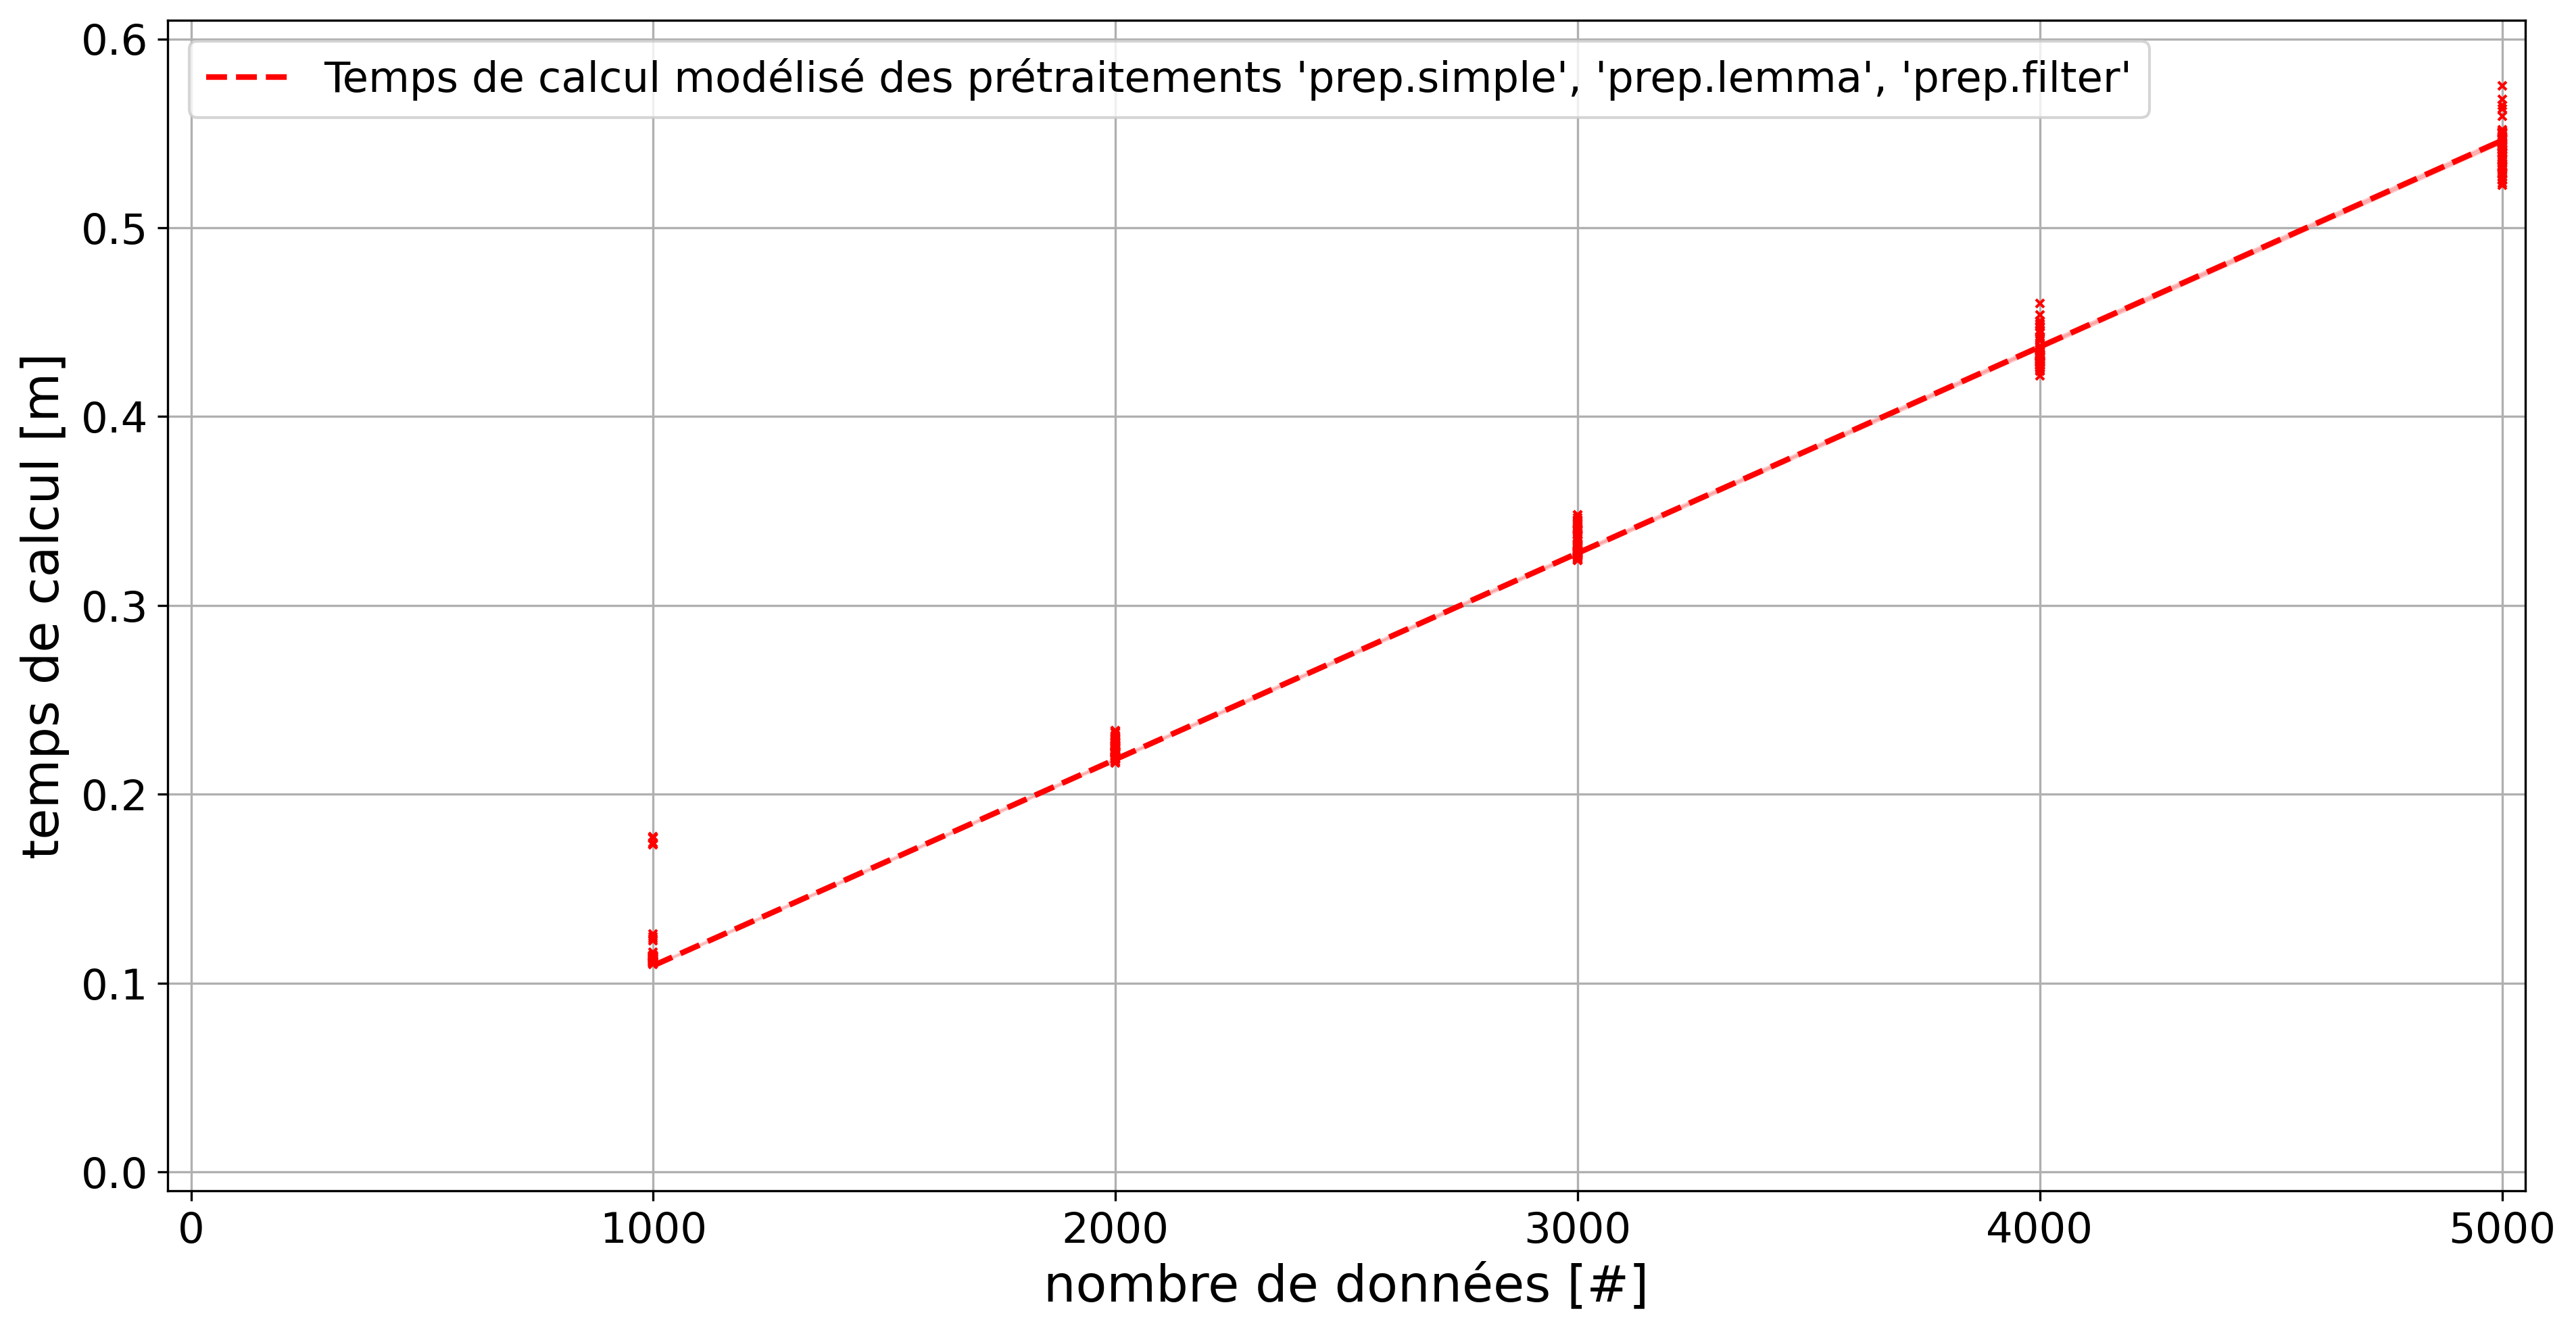
\includegraphics[width=0.95\textwidth]{figures/etude-temps-calcul-modelisation-1prep}
				\caption{
					Estimation du temps nécessaire (en minutes) pour effectuer une tâche de \textbf{prétraitements} en fonction du nombre de données à traiter. Les paramétrages \texttt{prep.simple}, \texttt{prep.lemma} et \texttt{prep.filter} ayant des temps de calculs similaires, leurs modélisations n'ont pas été séparées.
				}
				\label{figure:4.3.2-ETUDE-COUTS-TEMPS-CALCUL-MODELISATION-PREPROCESSING}
			\end{figure}
			
			%%% Vectorization
			
			% Première analyse.
			En ce qui concerne la tâche de \textbf{vectorisation}, une première analyse montre que les modélisations des deux implémentations sont différentiables (\texttt{p-valeur}: $< 10^{-3}$). Nous faisons donc une modélisation par algorithme.
		
			% Modélisation du temps de calcul (vect.tfidf).
			Pour les algorithmes de vectorisation \texttt{vect.tfidf}, l'analyse de la corrélation des facteurs avec les mesures de temps d'exécution indique qu'une modélisation minimale et suffisante peut être réalisée à partir du facteur $\texttt{dataset\_size}$ (\texttt{r}: $0.977$).
			Le modèle linéaire généralisé retenu (\texttt{R²}: $> 0.999$, \texttt{llf}: $259.89$, \texttt{llf\_null}: $70.04$) nous permet de déduire l'équation suivante :
			%
			\begin{equation}
				\texttt{computation\_time}(\texttt{vect.tfidf})~[s]~
				\propto~9.16 \cdot 10^{-5} \cdot \texttt{dataset\_size}
			\end{equation}
			
			% Modélisation du temps de calcul (vect.frcorenewsmd).
			Pour les algorithmes de vectorisation \texttt{vect.frcorenewsmd}, l'analyse de la corrélation des facteurs avec les mesures de temps d'exécution indique qu'une modélisation minimale et suffisante peut être réalisée à partir du facteur $\texttt{dataset\_size}$ (\texttt{r}: $0.983$).
			Le modèle linéaire généralisé retenu (\texttt{R²}: $> 0.999$, \texttt{llf}: $-214.44$, \texttt{llf\_null}: $-399.39$) nous permet de déduire l'équation suivante :
			%
			\begin{equation}
				\texttt{computation\_time}(\texttt{vect.frcorenewsmd})~[s]~
				\propto~4.62 \cdot 10^{-3} \cdot \texttt{dataset\_size}
			\end{equation}
			
			% Affichage du temps de calcul.
			La \textsc{Figure~\ref{figure:4.3.2-ETUDE-COUTS-TEMPS-CALCUL-MODELISATION-VECTORIZATION}} représente ces modélisations de temps de calcul des algorithmes de vectorisation en comparaison avec les mesures réalisées lors de l'expérience.
			\newline
			%
			\begin{figure}[!htb]
				\centering
				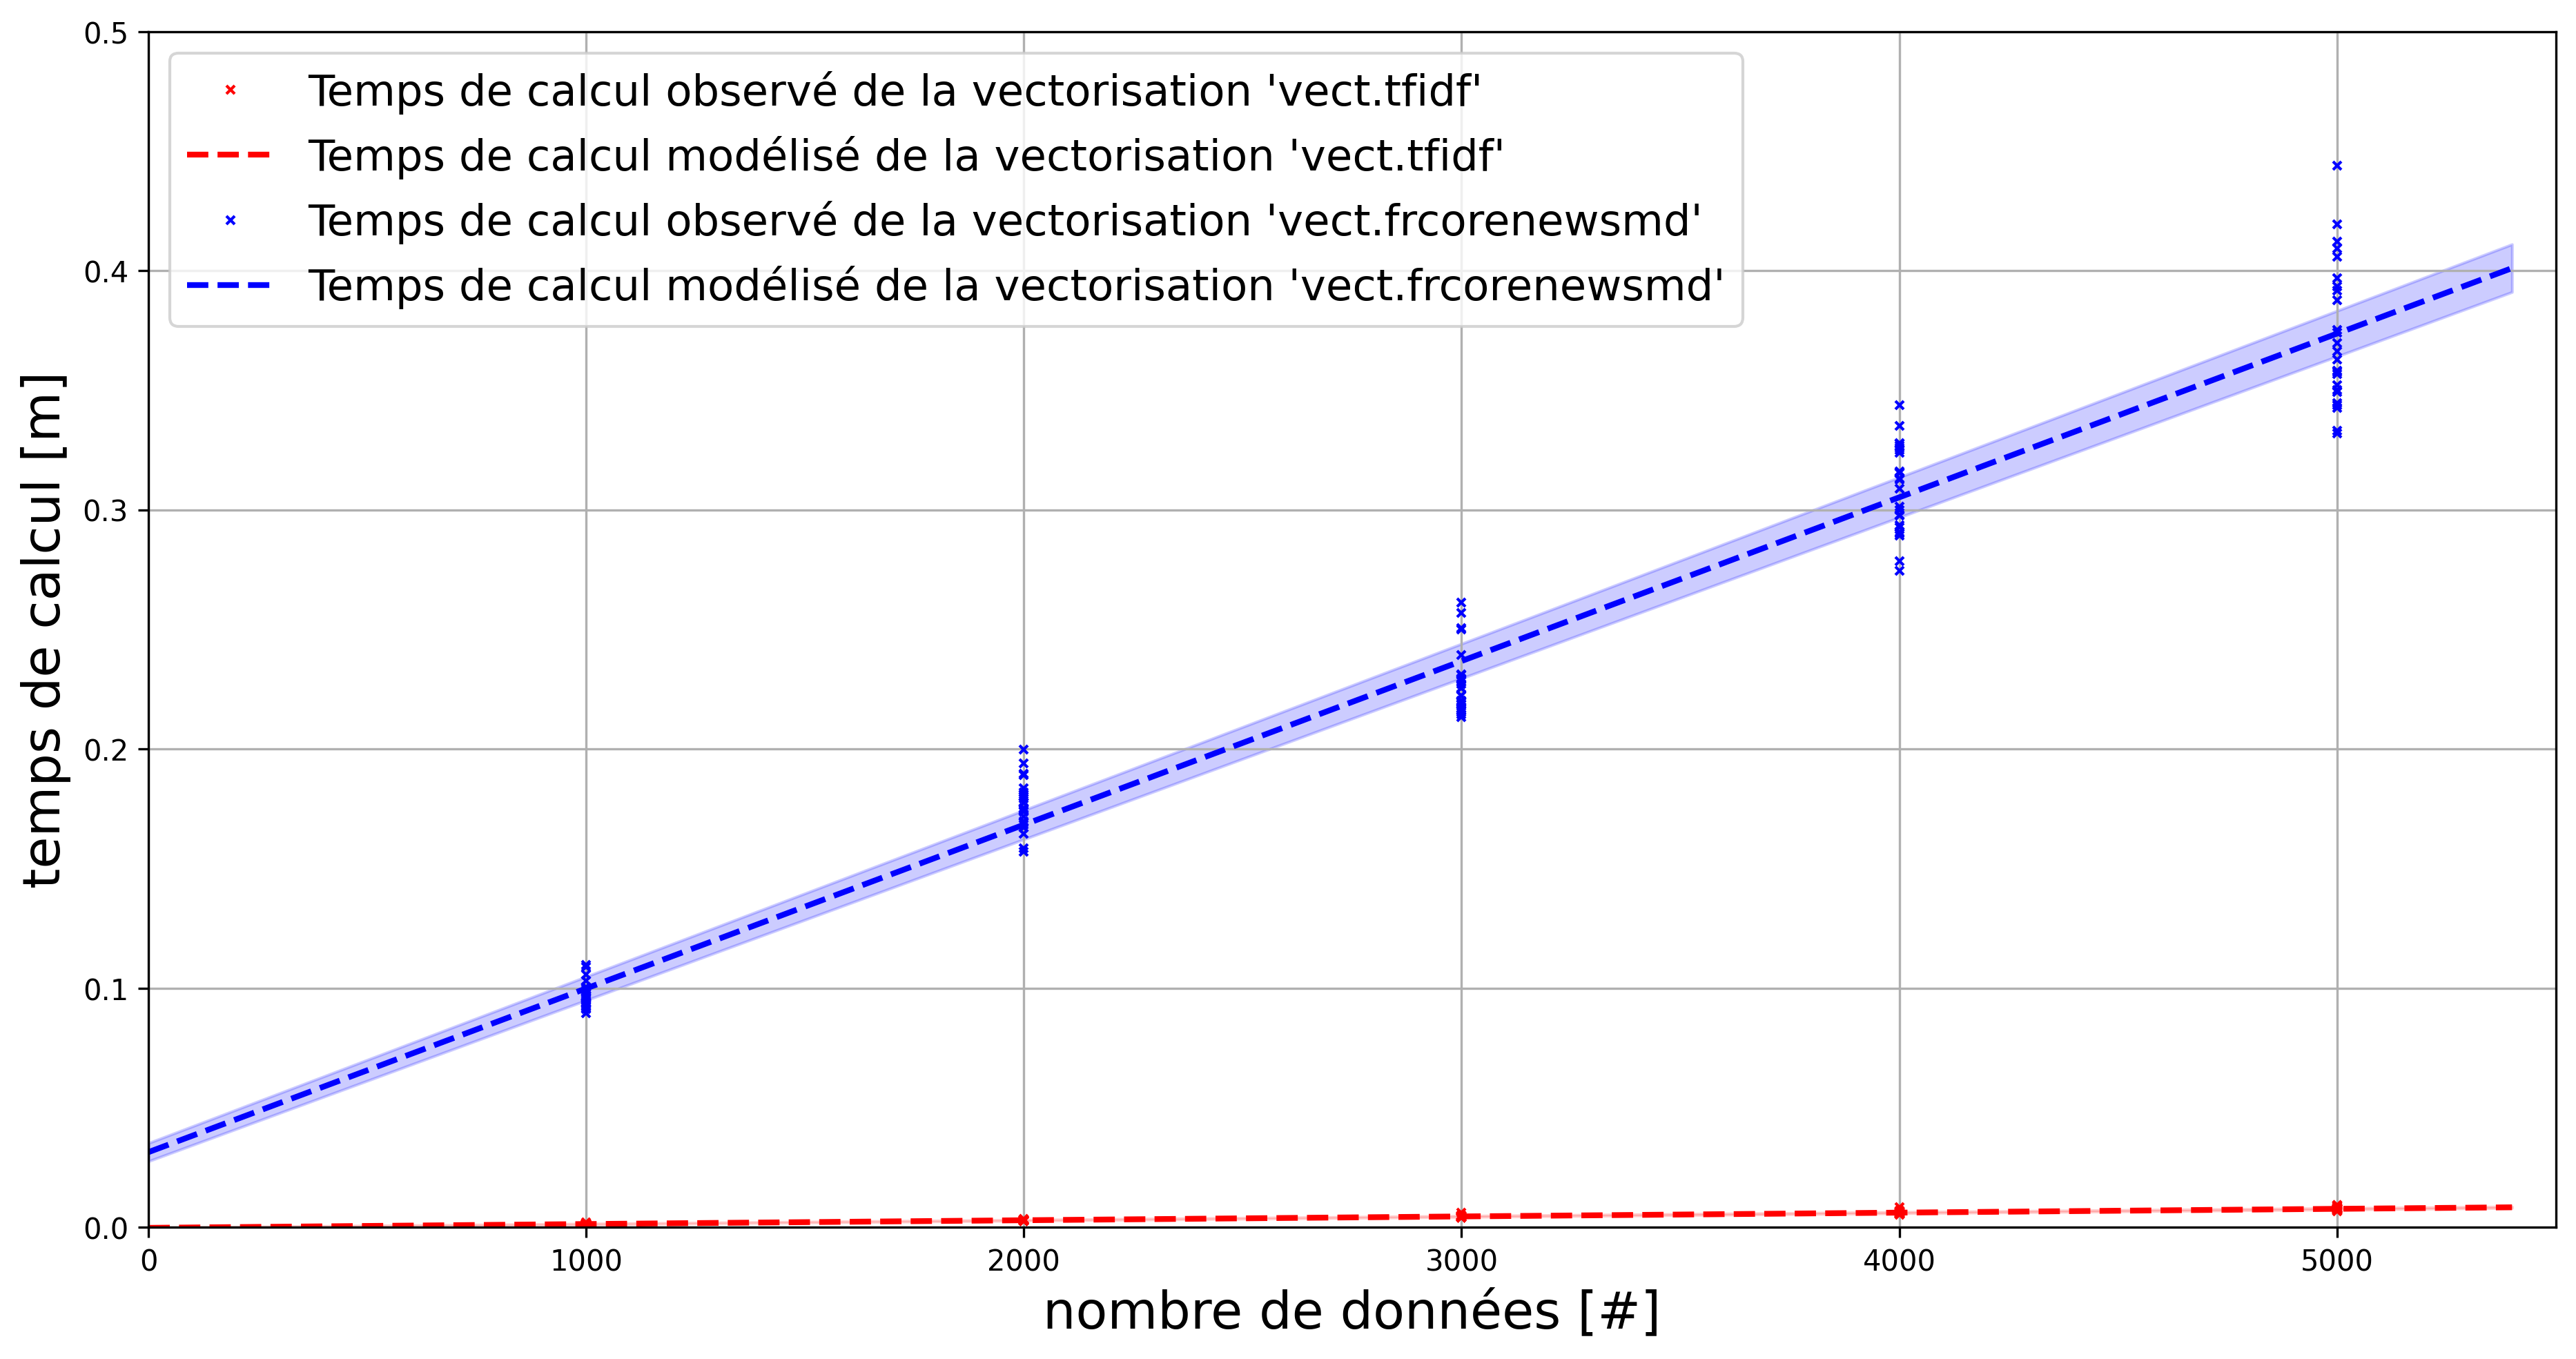
\includegraphics[width=0.95\textwidth]{figures/etude-temps-calcul-modelisation-2vect}
				\caption{
					Estimation du temps nécessaire (en minutes) pour effectuer une tâche de \textbf{vectorisation} en fonction du nombre de données à traiter.
				}
				\label{figure:4.3.2-ETUDE-COUTS-TEMPS-CALCUL-MODELISATION-VECTORIZATION}
			\end{figure}
			
			%%% \textit{Clustering}
			
			% Première analyse.
			En ce qui concerne la tâche de \textbf{\textit{clustering} sous contraintes}, une première analyse montre que les modélisations des six implémentations sont différentiables (\texttt{p-valeur}: $<$ \texttt{$10^{-3}$}). Nous faisons donc une modélisation par algorithme.
			
			% Remarques: hiérarchique trop long.
			\begin{leftBarWarning}
				Plusieurs exécutions des algorithmes de type \textit{hiérarchique} ont été annulées pour les jeux de données de tailles supérieures à $4~000$ car la durée excède plusieurs heures.
				Nous limitons donc l'analyse de \texttt{clust.hier.sing}, \texttt{clust.hier.comp}, \texttt{clust.hier.avg} et \texttt{clust.hier.ward} aux tailles de $1~000$ à $3~000$.
			\end{leftBarWarning}
			
			% Modélisation du temps de calcul (clust.kmeans.cop).
			Pour les algorithmes du \textit{clustering} sous contraintes \texttt{clust.kmeans.cop}, l'analyse de la corrélation des facteurs avec les mesures de temps d'exécution indique qu'une modélisation minimale et suffisante peut être réalisée à partir du facteur $\texttt{dataset\_size}$ (\texttt{r}: $0.837$).
			Le second facteur le plus corrélé (mais non retenu) est l'interaction $\texttt{dataset\_size}^{\textbf{2}} \cdot \texttt{algorithm\_nb\_clusters}$ (\texttt{r}: $0.545$).
			Le modèle linéaire généralisé retenu (\texttt{R²}: $0.802$, \texttt{llf}: $-9.37 \cdot 10^{4}$, \texttt{llf\_null}: $-1.00 \cdot 10^{5}$) nous permet de déduire l'équation suivante :
			%
			\begin{equation}
				\texttt{computation\_time}(\texttt{clust.kmeans.cop})~[s]~
				\propto~1.45 \cdot 10^{-1} \cdot \texttt{dataset\_size}
			\end{equation}
			
			% Modélisation du temps de calcul (clust.hier.sing).
			Pour les algorithmes du \textit{clustering} sous contraintes \texttt{clust.hier.sing}, l'analyse de la corrélation des facteurs avec les mesures de temps d'exécution indique qu'une modélisation minimale et suffisante peut être réalisée à partir du facteur $\texttt{dataset\_size}^{\textbf{2}}$ (\texttt{r}: $0.940$).
			Le second facteur le plus corrélé (mais non retenu) est l'interaction $\texttt{dataset\_size}^{\textbf{2}} \cdot \texttt{algorithm\_nb\_clusters}$ (\texttt{r}: $0.729$).
			Le modèle linéaire généralisé retenu (\texttt{R²}: $0.987$, \texttt{llf}: $-5.54 \cdot 10^{4}$, \texttt{llf\_null}: $-6.10 \cdot 10^{4}$) nous permet de déduire l'équation suivante :
			%
			\begin{equation}
				\texttt{computation\_time}(\texttt{clust.hier.sing})~[s]~
				\propto~5.00 \cdot 10^{-4} \cdot \texttt{dataset\_size}^{\textbf{2}}
			\end{equation}
			
			% Modélisation du temps de calcul (clust.hier.comp).
			Pour les algorithmes du \textit{clustering} sous contraintes \texttt{clust.hier.comp}, l'analyse de la corrélation des facteurs avec les mesures de temps d'exécution indique qu'une modélisation minimale et suffisante peut être réalisée à partir du facteur $\texttt{dataset\_size}^{\textbf{2}}$ (\texttt{r}: $0.938$).
			Le second facteur le plus corrélé (mais non retenu) est l'interaction $\texttt{dataset\_size}^{\textbf{2}} \cdot \texttt{algorithm\_nb\_clusters}$ (\texttt{r}: $0.736$).
			Le modèle linéaire généralisé retenu (\texttt{R²}: $0.984$, \texttt{llf}: $-5.56 \cdot 10^{4}$, \texttt{llf\_null}: $-6.11 \cdot 10^{4}$) nous permet de déduire l'équation suivante :
			%
			\begin{equation}
				\texttt{computation\_time}(\texttt{clust.hier.comp})~[s]~
				\propto~4.99 \cdot 10^{-4} \cdot \texttt{dataset\_size}^{\textbf{2}}
			\end{equation}

			% Modélisation du temps de calcul (clust.hier.avg).
			Pour les algorithmes du \textit{clustering} sous contraintes \texttt{clust.hier.avg}, l'analyse de la corrélation des facteurs avec les mesures de temps d'exécution indique qu'une modélisation minimale et suffisante peut être réalisée à partir du facteur $\texttt{dataset\_size}^{\textbf{2}}$ (\texttt{r}: $0.915$).
			Le second facteur le plus corrélé (mais non retenu) est l'interaction $\texttt{dataset\_size}^{\textbf{2}} \cdot \texttt{algorithm\_nb\_clusters}$ (\texttt{r}: $0.713$).
			Le modèle linéaire généralisé retenu (\texttt{R²}: $0.981$, \texttt{llf}: $-5.90 \cdot 10^{4}$, \texttt{llf\_null}: $-6.45 \cdot 10^{4}$) nous permet de déduire l'équation suivante :
			%
			\begin{equation}
				\texttt{computation\_time}(\texttt{clust.hier.avg})~[s]~
				\propto~8.51 \cdot 10^{-4} \cdot \texttt{dataset\_size}^{\textbf{2}}
			\end{equation}

			% Modélisation du temps de calcul (clust.hier.ward).
			Pour les algorithmes du \textit{clustering} sous contraintes \texttt{clust.hier.ward}, l'analyse de la corrélation des facteurs avec les mesures de temps d'exécution indique qu'une modélisation minimale et suffisante peut être réalisée à partir du facteur $\texttt{dataset\_size}^{\textbf{2}}$ (\texttt{r}: $0.945$).
			Le second facteur le plus corrélé (mais non retenu) est l'interaction $\texttt{dataset\_size}^{\textbf{2}} \cdot \texttt{algorithm\_nb\_clusters}$ (\texttt{r}: $0.734$).
			Le modèle linéaire généralisé retenu (\texttt{R²}: $0.989$, \texttt{llf}: $-5.57 \cdot 10^{4}$, \texttt{llf\_null}: $-6.14 \cdot 10^{4}$) nous permet de déduire l'équation suivante :
			%
			\begin{equation}
				\texttt{computation\_time}(\texttt{clust.hier.ward})~[s]~
				\propto~5.30 \cdot 10^{-4} \cdot \texttt{dataset\_size}^{\textbf{2}}
			\end{equation}
			
			% Modélisation du temps de calcul (clust.spec).
			Pour les algorithmes du \textit{clustering} sous contraintes \texttt{clust.spec}, l'analyse de la corrélation des facteurs avec les mesures de temps d'exécution indique qu'une modélisation minimale et suffisante peut être réalisée à partir du facteur $\texttt{dataset\_size}^{\textbf{2}}$ (\texttt{r}: $0.658$).
			Le second facteur le plus corrélé (mais non retenu) est l'interaction $\texttt{dataset\_size}^{\textbf{2}} \cdot \texttt{algorithm\_nb\_clusters}$ (\texttt{r}: $0.595$).
			Le modèle linéaire généralisé retenu (\texttt{R²}: $0.527$, \texttt{llf}: $-7.89 \cdot 10^{5}$, \texttt{llf\_null}: $-8.27 \cdot 10^{5}$) nous permet de déduire l'équation suivante :
			%
			\begin{equation}
				\texttt{computation\_time}(\texttt{clust.spec})~[s]~
				\propto~8.18 \cdot 10^{-6} \cdot \texttt{dataset\_size}^{\textbf{2}}
			\end{equation}
			
			% Affichage du temps de calcul.
			La \textsc{Figure~\ref{figure:4.3.2-ETUDE-COUTS-TEMPS-CALCUL-MODELISATION-CLUSTERING}} représente ces modélisations de temps de calcul des algorithmes de \textit{clustering} en comparaison avec les mesures réalisées lors de l'expérience.
			\newline
			%
			\begin{figure}[!htb]
				\centering
				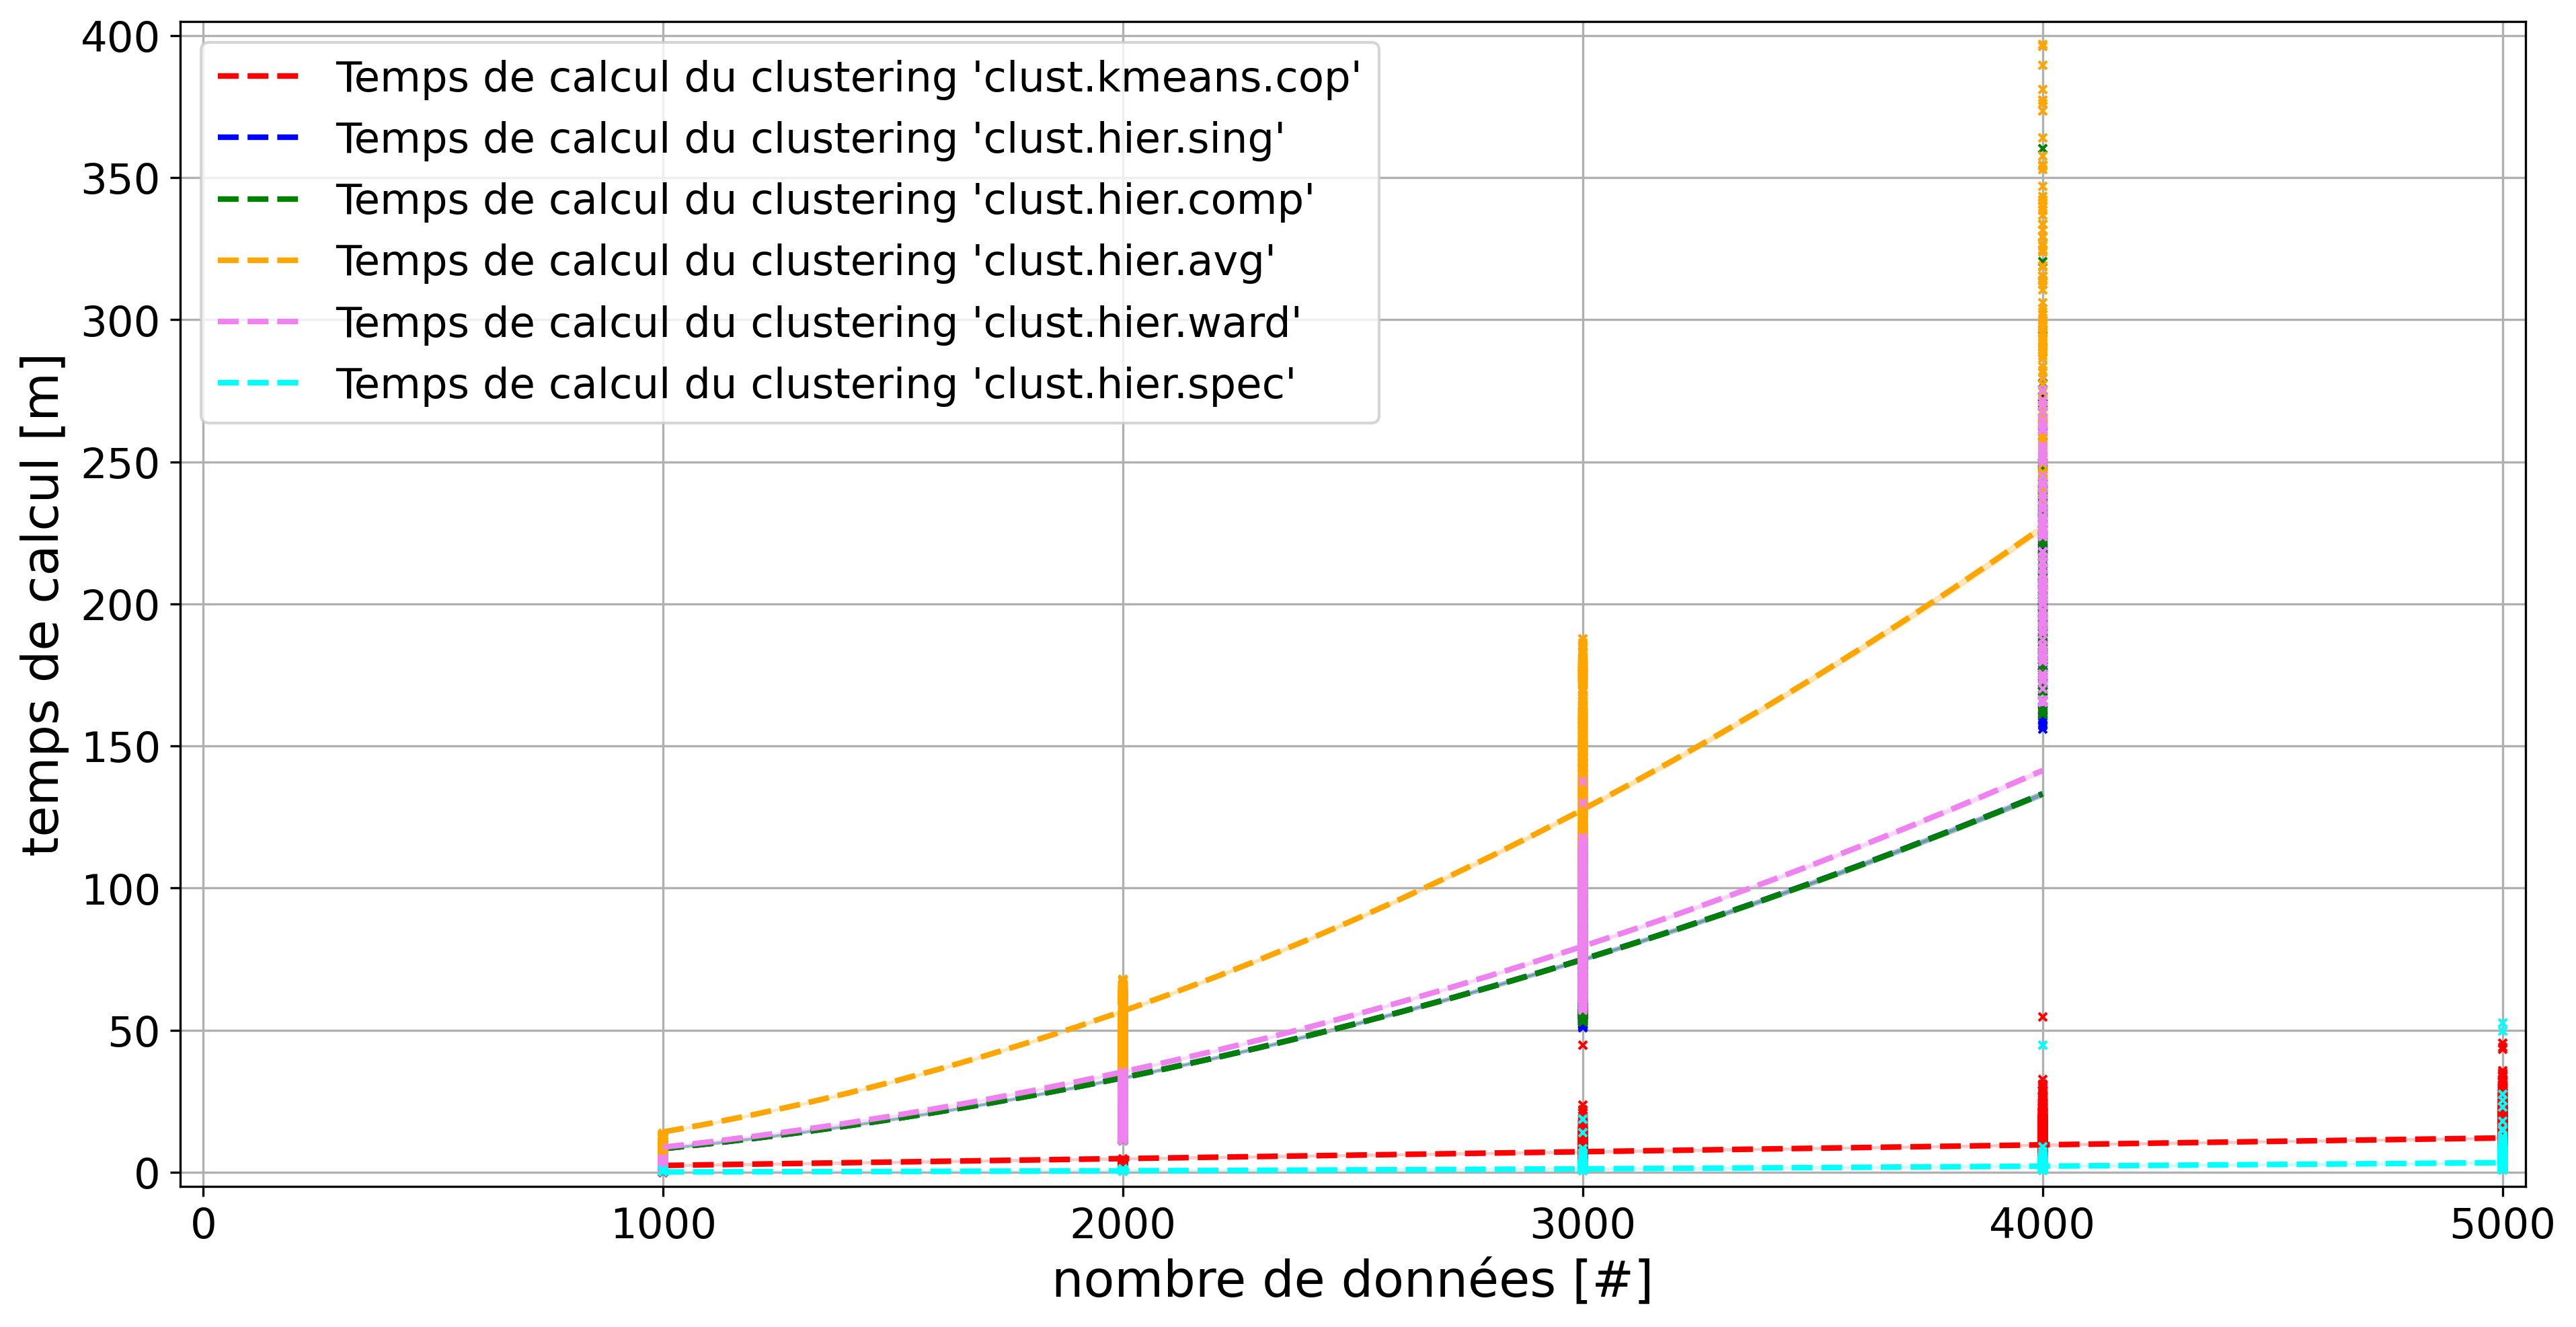
\includegraphics[width=0.95\textwidth]{figures/etude-temps-calcul-modelisation-3clust}
				\caption{
					Estimation du temps nécessaire (en minutes) pour effectuer une tâche de \textbf{clustering} en fonction du nombre de données à traiter.
				}
				\label{figure:4.3.2-ETUDE-COUTS-TEMPS-CALCUL-MODELISATION-CLUSTERING}
			\end{figure}
			
			%%% Sampling
			
			% Première analyse.
			En ce qui concerne la tâche d'\textbf{échantillonnage de contraintes}, une première analyse montre que les modélisations des quatre implémentations sont différentiables  (\texttt{p-valeur}: $<$ \texttt{$10^{-3}$}). Nous faisons donc une modélisation par algorithme.
			
			% Modélisation du temps de calcul (samp.rand.full).
			Pour les algorithmes de l'échantillonnage de contraintes \texttt{samp.rand.full}, l'analyse de la corrélation des facteurs avec les mesures de temps d'exécution indique qu'une modélisation minimale et suffisante peut être réalisée à partir du facteur $\texttt{dataset\_size}^{\textbf{2}}$ (\texttt{r}: $0.993$).
			Le second facteur le plus corrélé (mais non retenu) est l'interaction $\texttt{dataset\_size}^{\textbf{2}} \cdot \texttt{previous\_nb\_clusters}$ (\texttt{r}: $0.791$).
			Le modèle linéaire généralisé retenu (\texttt{R²}: $> 0.999$, \texttt{llf}: $-4.52 \cdot 10^{4}$, \texttt{llf\_null}: $-1.17 \cdot 10^{5}$) nous permet de déduire l'équation suivante :
			%
			\begin{equation}
				\texttt{computation\_time}(\texttt{samp.rand.full})~[s]~
				\propto~8.20 \cdot 10^{-7} \cdot \texttt{dataset\_size}^{\textbf{2}}
			\end{equation}
			
			% Modélisation du temps de calcul (samp.rand.same).
			Pour les algorithmes de l'échantillonnage de contraintes \texttt{samp.rand.same}, l'analyse de la corrélation des facteurs avec les mesures de temps d'exécution indique qu'une modélisation minimale et suffisante peut être réalisée à partir du facteur $\texttt{dataset\_size}^{\textbf{2}}$ (\texttt{r}: $0.939$).
			Le second facteur le plus corrélé (mais non retenu) est l'interaction $\texttt{dataset\_size}^{\textbf{2}} \cdot \texttt{algorithm\_nb\_constraints}$ (\texttt{r}: $0.611$).
			Le modèle linéaire généralisé retenu (\texttt{R²}: $> 0.999$, \texttt{llf}: $-3.20 \cdot 10^{4}$, \texttt{llf\_null}: $-6.84 \cdot 10^{4}$) nous permet de déduire l'équation suivante :
			%
			\begin{equation}
				\texttt{computation\_time}(\texttt{samp.rand.same})~[s]~
				\propto~1.85 \cdot 10^{-7} \cdot \texttt{dataset\_size}^{\textbf{2}}
			\end{equation}
			
			% Modélisation du temps de calcul (samp.farthest.same).
			Pour les algorithmes de l'échantillonnage de contraintes \texttt{samp.farthest.same}, l'analyse de la corrélation des facteurs avec les mesures de temps d'exécution indique qu'une modélisation minimale et suffisante peut être réalisée à partir du facteur $\texttt{dataset\_size}^{\textbf{2}}$ (\texttt{r}: $0.981$).
			Le second facteur le plus corrélé (mais non retenu) est l'interaction $\texttt{dataset\_size}^{\textbf{2}} \cdot \texttt{previous\_nb\_clusters}$ (\texttt{r}: $0.700$).
			Le modèle linéaire généralisé retenu (\texttt{R²}: $> 0.999$, \texttt{llf}: $-4.56 \cdot 10^{4}$, \texttt{llf\_null}: $-1.02 \cdot 10^{5}$) nous permet de déduire l'équation suivante :
			%
			\begin{equation}
				\texttt{computation\_time}(\texttt{samp.farthest.same})~[s]~
				\propto~5.19 \cdot 10^{-7} \cdot \texttt{dataset\_size}^{\textbf{2}}
			\end{equation}
			
			% Modélisation du temps de calcul (samp.closest.diff).
			Pour les algorithmes de l'échantillonnage de contraintes \texttt{samp.closest.diff}, l'analyse de la corrélation des facteurs avec les mesures de temps d'exécution indique qu'une modélisation minimale et suffisante peut être réalisée à partir du facteur $\texttt{dataset\_size}^{\textbf{2}}$ (\texttt{r}: $0.995$).
			Le second facteur le plus corrélé (mais non retenu) est l'interaction $\texttt{dataset\_size}^{\textbf{2}} \cdot \texttt{previous\_nb\_clusters}$ (\texttt{r}: $0.815$).
			Le modèle linéaire généralisé retenu (\texttt{R²}: $> 0.999$, \texttt{llf}: $-5.96 \cdot 10^{4}$, \texttt{llf\_null}: $-1.36 \cdot 10^{5}$) nous permet de déduire l'équation suivante :
			%
			\begin{equation}
				\texttt{computation\_time}(\texttt{samp.closest.diff})~[s]~
				\propto~1.43 \cdot 10^{-6} \cdot \texttt{dataset\_size}^{\textbf{2}}
			\end{equation}
			
			% Affichage du temps de calcul.
			La \textsc{Figure~\ref{figure:4.3.2-ETUDE-COUTS-TEMPS-CALCUL-MODELISATION-SAMPLING}} représente ces modélisations de temps de calcul des algorithmes d'échantillonnage en comparaison avec les mesures réalisées lors de l'expérience.
			\newline
			%
			\begin{figure}[!htb]
				\centering
				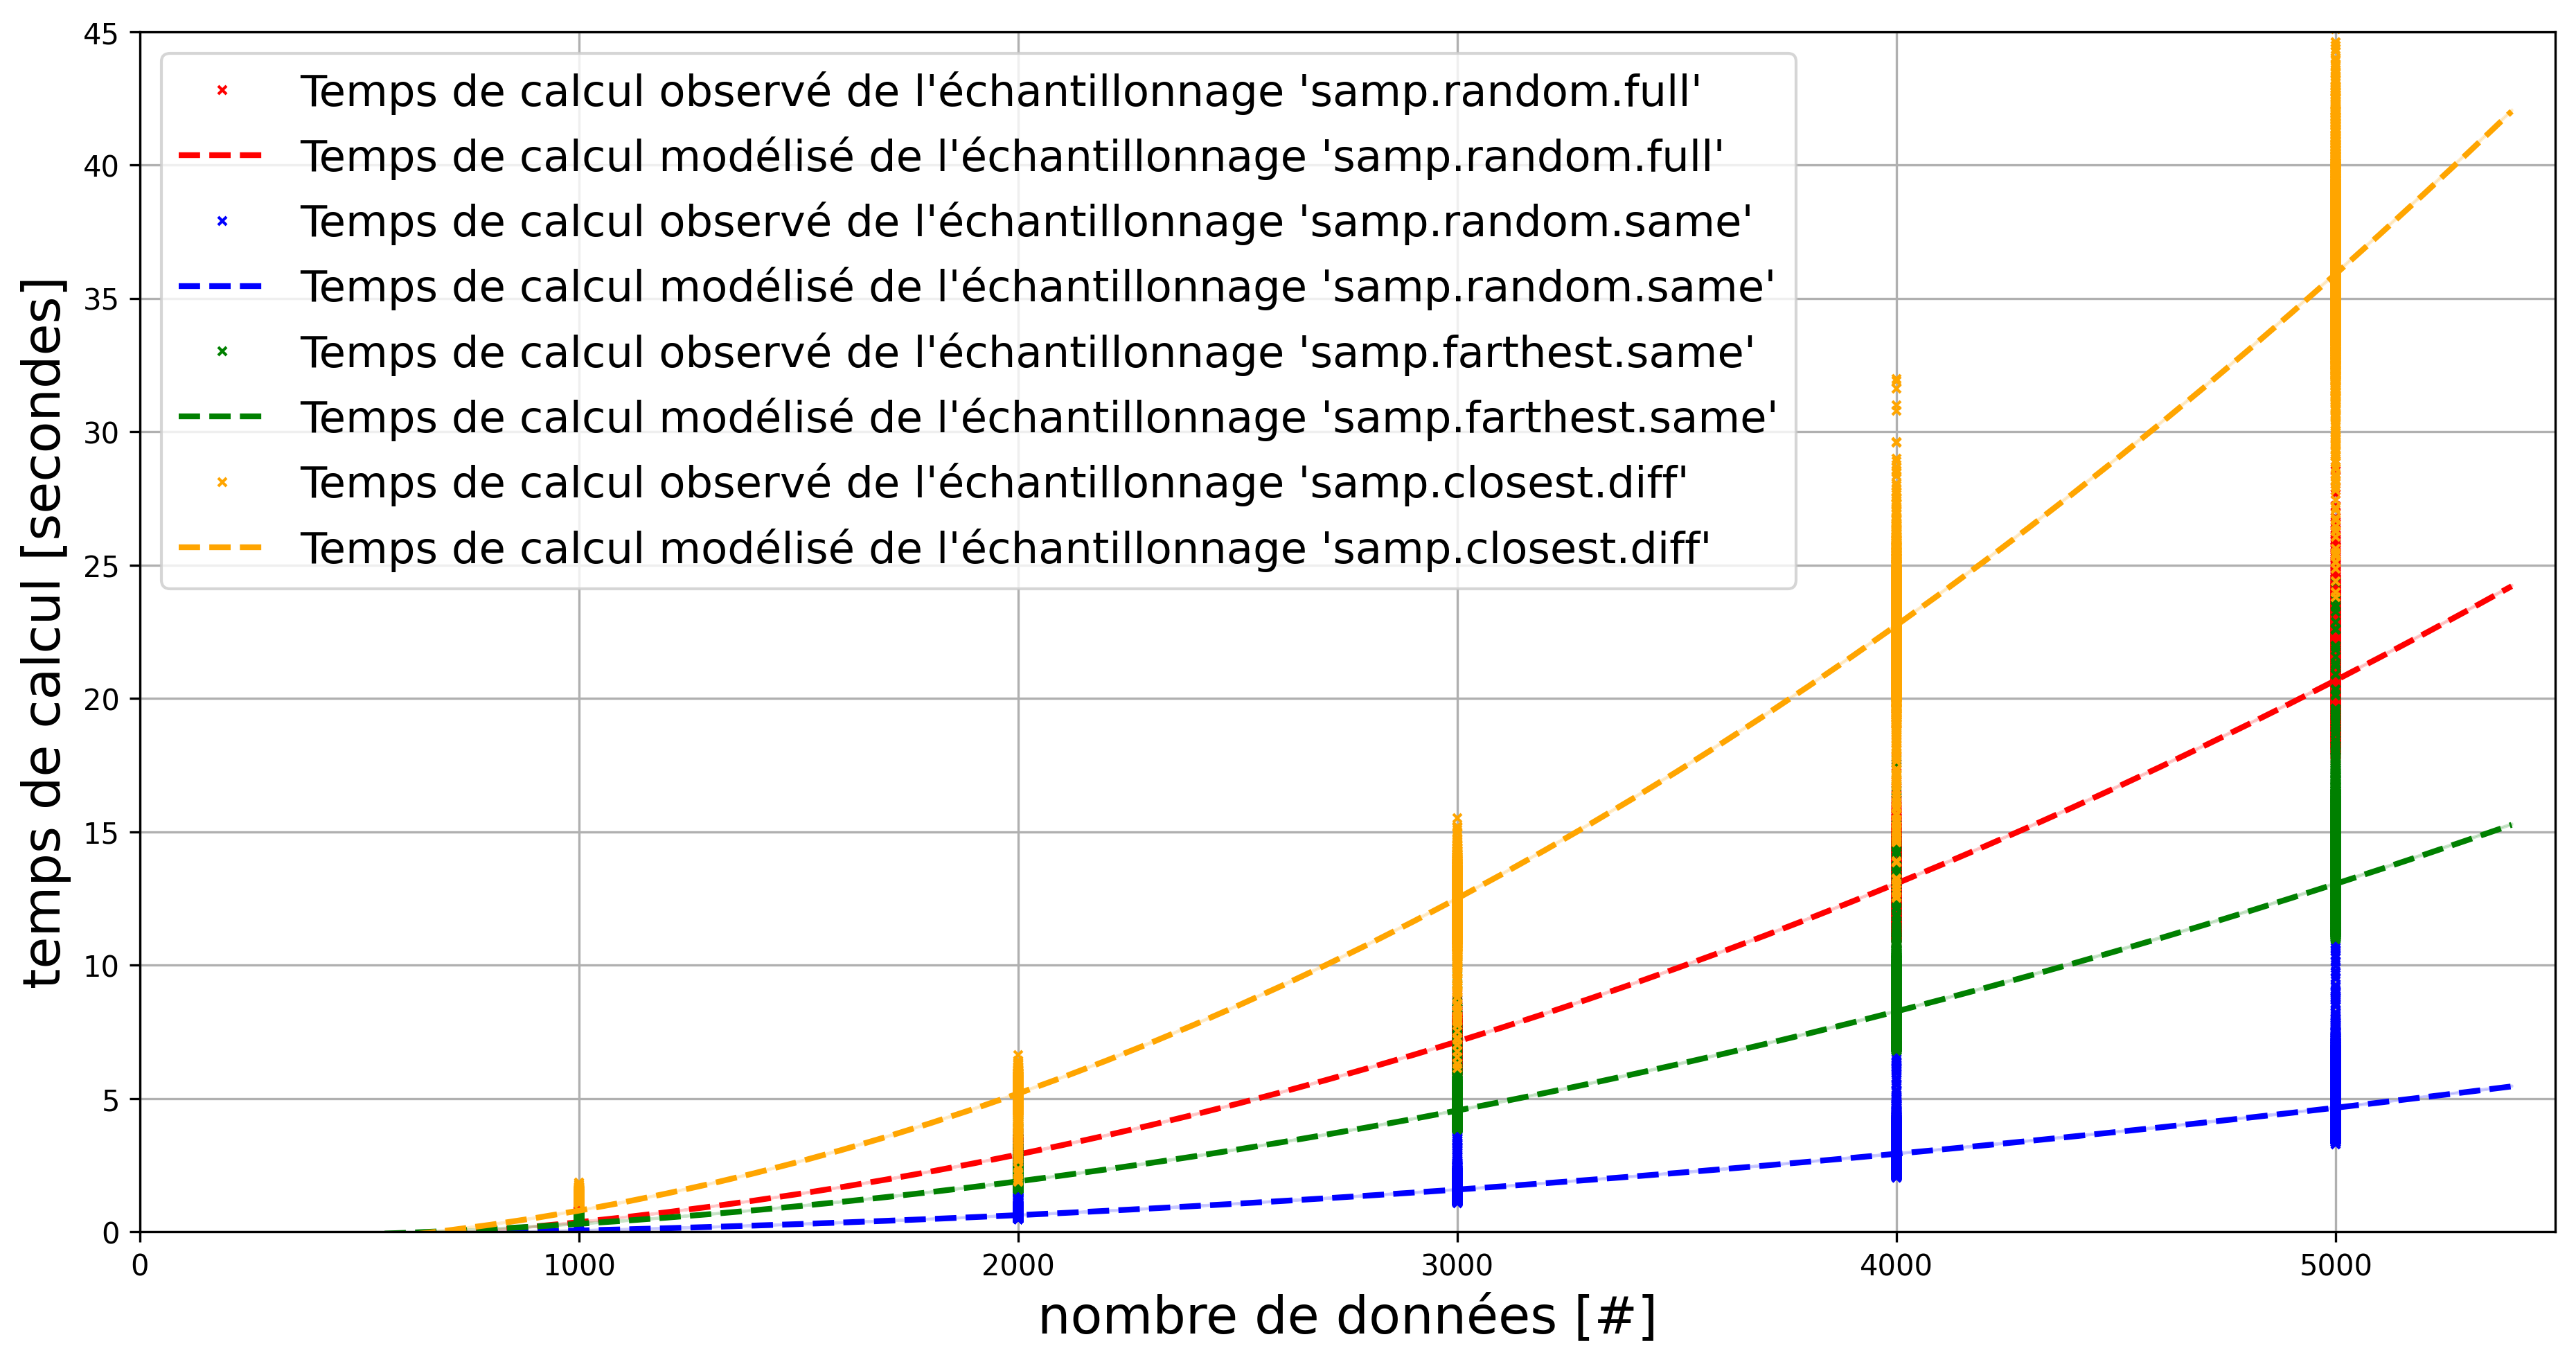
\includegraphics[width=0.95\textwidth]{figures/etude-temps-calcul-modelisation-4samp}
				\caption{
					Estimation du temps nécessaire (en minutes) pour effectuer une tâche d'\textbf{échantillonnage de contraintes} en fonction du nombre de données à traiter.
				}
				\label{figure:4.3.2-ETUDE-COUTS-TEMPS-CALCUL-MODELISATION-SAMPLING}
			\end{figure}

		%%% Discussion.
		\subsubsection{Discussion}
		
			% Rappel de l'objectif : estimer le temps d'exécution.
			Dans cette étude, nous avons estimé le temps de calcul des différents algorithmes implémentés afin de confirmer le choix de paramétrage pour une convergence optimale (cf. hypothèse d'efficience en \textsc{Section~\ref{section:4.2-HYPOTHESE-EFFICIENCE}}).
			Ces estimations ont été réalisées sur la base de plusieurs exécutions et fonction de divers contextes d'utilisation : nombre de données, nombre de contraintes annotées, nombre de contraintes à sélectionner, nombre de \textit{clusters} existants, nombre de \textit{clusters} à trouver.
			\\
			
			% Remarque générale : Dépend principalement du nombre de données.
			En premier lieu, nous pouvons constater que les différentes modélisations dépendent majoritairement de la taille du jeu de données manipulé ($\texttt{dataset\_size}$ ou $\texttt{dataset\_size}^{\textbf{2}}$) avec un score de corrélation \texttt{r} avec le temps mesuré généralement supérieur à $0.9$ et des modèles \textit{GLM} avec des coefficients de détermination généralisé \texttt{R²} généralement proches de $0.999$.
			Bien que d'autres facteurs peuvent intervenir dans ces estimations (notamment les interactions doubles entre la taille du jeu de données et le nombre de \textit{clusters} ou le nombre de contraintes), ces derniers semblent avoir un impact négligeable sur le temps d'exécution.
			
			% Note: remarque sur le nombre de contraintes.
			\begin{leftBarAuthorOpinion}
				Certains paramétrages de la méthode du \texttt{Clustering Interactif} semblent cependant avoir un temps de calcul décroissant au cours des itérations, mais nous n'avons cependant pas pu montrer de tendances globales significatives.
				Il est probable que l'ajout de contraintes judicieusement placées permettent à certains algorithmes de \textit{clustering} de s'exécuter plus rapidement, notamment lorsque ceux-ci exploitent les composants connexes du graphe de contraintes (cf. \textsc{Annexe~\ref{annex:C.1.2-DESCRIPTION-IMPLEMENTATION-INTERACTIVE-CLUSTERING-GESTION-DES-CONTRAINTES}}).
				En effet, :
				\begin{itemize}
					\item les \textit{clustering} hiérarchiques s'initialisent avec autant de \textit{clusters} que de groupes de données liées entre elles par des contraintes \texttt{MUST-LINK} : or s'il y a plus de contraintes, alors les composants connexes sont davantage développés, donc il y a moins de \textit{clusters} à initialiser et donc moins d'époques de l'algorithme ;
					\item le \textit{clustering} \texttt{KMeans} (modèle \texttt{COP}) attire auprès d'un barycentre l'ensemble des données liées par un \texttt{MUST-LINK} : or s'il y a plus de contraintes, alors il y a des données attirées, donc les noyaux de \textit{clusters} peuvent se stabiliser plus rapidement.  
				\end{itemize}
				Toutefois, ces suppositions n'ont pas pu être démontrées, et certains contre-exemples tendent à conclure que ces comportements sont très dépendants du jeu de données manipulé et de l'ordre d'ajout des contraintes. Par exemple :
				\begin{itemize}
					\item l'ajout d'un trop grand nombre de contraintes \texttt{CANNOT-LINK} peut engendrer un surplus de vérifications pour estimer quelles formations de \textit{clusters} sont autorisées sans violer de contraintes ;
					\item l'algorithme \texttt{KMeans} (modèle \texttt{COP}) peut osciller autour de plusieurs noyaux de \textit{clusters} instables si les contraintes violent trop la similarité intrinsèque des données.
				\end{itemize}
			\end{leftBarAuthorOpinion}
			
			% Cas du \textit{clustering}.
			En ce qui concerne la tâche de \textit{clustering}, nous notons des différences significatives dans les temps d'exécution des divers algorithmes implémentés.
			En effet, l'algorithme \texttt{KMeans} (modèle \texttt{COP}) est nettement plus rapide (complexité estimée en $ \mathcal{O}(\texttt{dataset\_size}) $, nécessitant quelques dizaines de minutes pour $5~000$ données) que les implémentations du \textit{clustering} hiérarchique (complexité estimée en $ \mathcal{O}(\texttt{dataset\_size}^{\textbf{2}}) $, nécessitant plusieurs heures dès $3~000$ données).
			Cette différence, visible en \textsc{Figure~\ref{figure:4.3.2-ETUDE-COUTS-TEMPS-CALCUL-MODELISATION-CLUSTERING}}, a un réel impact sur l'expérience utilisateur de l'opérateur.
			En effet, bien qu'il soit théoriquement plus efficient pour atteindre une annotation suffisante (cf. hypothèse d'efficience en \textsc{Section~\ref{section:4.2-HYPOTHESE-EFFICIENCE}}), l'usage d'un \textit{clustering} hiérarchique imposerait de longs temps d'attente à l'opérateur, interdisant des interactions rapides avec la machine.
			Or l'intérêt principal de notre méthodologie d'annotation à l'aide du \texttt{Clustering Interactif} repose sur ces interactions Homme/Machine via l'ajout régulier de contraintes pertinentes (cf. hypothèse d'efficacité en \textsc{Section~\ref{section:4.1-HYPOTHESE-EFFICACITE}}).
			Nous décidons donc d'exclure l'usage des algorithmes de \textit{clustering} hiérarchique au profit du \textit{clustering} \texttt{KMeans} (modèle \texttt{COP}).
			
			% Note: Cas du projet étudiant avec TPS.
			\begin{leftBarInformation}
				Dans le cadre d'un projet étudiants avec l'École d'Ingénieurs Télécom Physique Strasbourg (au cours de l'année 2022) visant à implémenter d'autres algorithmes de \textit{clustering} sous contraintes, un raisonnement similaire a été utilisé pour filtrer les algorithmes.
				Ainsi, l'implémentation de \texttt{KMeans} (modèle \texttt{MPC}) a été exclue (complexité estimée en $ \mathcal{O}(\texttt{dataset\_size}^{\textbf{3}}) $) et l'implémentation de la propagation par affinité écarte la gestion des contraintes \texttt{CANNOT-LINK} pour avoir un temps d'exécution comparable au \textit{clustering} KMeans (modèle COP).
				L'algorithme \texttt{DBScan} (modèle \texttt{C-DBScan}) est quant à lui un rival possible avec une complexité estimée en $ \mathcal{O}(\texttt{dataset\_size}) $.
			\end{leftBarInformation}
			
			% Cas du prétraitements + vectorisation + échantillonnage.
			Les tâches de prétraitements (cf. \textsc{Figure~\ref{figure:4.3.2-ETUDE-COUTS-TEMPS-CALCUL-MODELISATION-PREPROCESSING}}), de vectorisation (cf. \textsc{Figure~\ref{figure:4.3.2-ETUDE-COUTS-TEMPS-CALCUL-MODELISATION-VECTORIZATION}}), et d'échantillonnage de contraintes (cf. \textsc{Figure~\ref{figure:4.3.2-ETUDE-COUTS-TEMPS-CALCUL-MODELISATION-SAMPLING}}) ont des complexités presque négligeables en représentant moins de $10$\% des temps d'exécution du \textit{clustering} (pour $5~000$ données : moins de $1$ minute pour les trois algorithmes, contre $12.1$ minutes pour \texttt{clust.kmeans.cop} et $3.5$ heures pour \texttt{clust.hier.sing}).
			Nous maintenons donc les paramétrages obtenus pour ces tâches en \textsc{Section~\ref{section:4.2-HYPOTHESE-EFFICIENCE}} sans analyses complémentaires, et nous utilisons l'estimation temporelle du \textit{clustering} \texttt{clust.kmeans.cop} majorée de $10$\%.
			
			% Conclusion.
			\setcounter{localCounterOfFootnoteValue}{\value{footnote}}
			\begin{leftBarSummary}
				Dans l'optique d'atteindre de manière efficiente $90$\% de \texttt{v-measure} \footnotemark avec un coût global minimal, nous retenons l'usage du \textbf{paramétrage favori} constitué des prétraitements simples (\texttt{prep.simple}), de la vectorisation \texttt{TF-IDF} (\texttt{vect.tfidf}), du \textit{clustering} \texttt{KMeans} avec modèle \texttt{COP} (\texttt{clust.kmeans.cop}) et de l'échantillonnage des données les plus proches dans des \textit{clusters} différents (\texttt{sampl.closest.diff}).
				Nous estimons le temps d'exécution de ce paramétrage avec l'équation suivante \footnotemark :
				%
				\begin{equation}
					\label{equation:4.3.2-ETUDE-COUTS-TEMPS-CALCUL-PARAMETRAGE-FAVORI}
					\texttt{computation\_time}(\texttt{settings.favorite})~[s]~
					\propto~0.17 \cdot \texttt{dataset\_size}
				\end{equation}
			\end{leftBarSummary}
			% Rattraper les footnote.
				\stepcounter{localCounterOfFootnoteValue}
				\footnotetext[\value{localCounterOfFootnoteValue}]{
					$90$\% de \texttt{v-measure}: cas d'une annotation dite partielle, dont le paramétrage le plus efficient est constitué des prétraitements simples (\texttt{prep.simple}), de la vectorisation \texttt{TF-IDF} (\texttt{vect.tfidf}), du \textit{clustering} hiérarchique à lien moyen (\texttt{clust.hier.avg}) et de l'échantillonnage des données les plus proches dans des \textit{clusters} différents (\texttt{sampl.closest.diff}).
				}
				\stepcounter{localCounterOfFootnoteValue}
				\footnotetext[\value{localCounterOfFootnoteValue}]{
					Temps du paramétrage favori : environ $2.8$ minutes pour $1~000$ données ; environ $14.2$ minutes pour $5~000$ données.
				}
	
	%%%
	%%% Subsection 4.3.3: Étude du nombre de contraintes nécessaires à la convergence vers une vérité terrain préétablie en fonction de la taille du jeu de données 
	%%%
	\subsection{Étude du nombre de contraintes nécessaires à la convergence vers une vérité terrain préétablie en fonction de la taille du jeu de données}
	\label{section:4.3.3-ETUDE-COUT-NOMBRE-CONTRAINTES}
			
		% Transition.
		Avec les deux précédentes études, nous sommes capable d'estimer le temps nécessaire à un expert pour annoter des contraintes, et le temps nécessaire à la machine pour proposer un nouveau \textit{clustering} adapté aux suggestions de l'expert.
		Pour poursuivre nos études et pouvoir estimer le coût total d'un projet d'annotation, il nous reste à estimer le nombre total de contraintes à devoir renseigner en fonction de la taille du jeu de données.
		
		% Objectif de l'expérience.
		Pour cela, nous allons simuler la création de cette base d'apprentissage en adaptant le protocole utilisé lors de notre étude d'efficacité (cf. \textsc{Section~\ref{section:4.1.1-ETUDE-CONVERGENCE}}) :
		nous employons notre méthode de \texttt{Clustering Interactif} avec notre \textbf{paramétrage favori} \footnote{
			Paramétrage favori (atteindre $90$\% de \texttt{v-measure} avec un coût minimal): prétraitements simples (\texttt{prep.simple}), vectorisation \texttt{TF-IDF} (\texttt{vect.tfidf}), \textit{clustering} \texttt{KMeans} avec modèle \texttt{COP} (\texttt{clust.kmeans.cop}) et échantillonnage des données les plus proches dans des \textit{clusters} différents (\texttt{sampl.closest.diff}).
		} sur des jeux de données de différentes tailles et mesurons le nombre de contraintes nécessaires pour converger vers la vérité terrain.
	
		%%% Protocole expérimental.
		\subsubsection{Protocole expérimental}
			
			% Axiome.
			\begin{leftBarWarning}
				Dans le cadre de cette étude, nous supposons que l'expert métier connaît parfaitement le domaine traité dans ce jeu de données, et qu'il est capable de caractériser sans ambiguïté la similitude entre deux données issues de cet ensemble.
			\end{leftBarWarning}
			
			% Pseudo-code.
			Pour résumer le protocole expérimental que nous détaillons ci-dessous, une description en pseudo-code est disponible dans l'\textsc{Algorithme~\ref{algorithm:4.3.3-ETUDE-COUT-NOMBRE-CONTRAINTES-PROTOCOLE}}.
			
			\begin{algorithm}
				\KwData{jeux de données annotées (vérités terrains) de tailles différentes}
				%
				\ForEach{jeux de données à tester}{
					\textbf{initialisation (données)}: récupérer ou générer les données et la vérité terrain \;
					\textbf{initialisation (contraintes)}: créer une liste vide de contraintes \;
					\textbf{prétraitements}: supprimer le bruit dans les données avec \texttt{prep.simple} \;
					\textbf{vectorisation}: transformer les données en vecteurs avec \texttt{vect.tfidf} \;
					\textbf{clustering initial}: regrouper les données par similarité avec \texttt{clust.kmeans.cop} \;
					\textbf{évaluation}: estimer l'équivalence entre le \textit{clustering} et la vérité terrain \;
					\Repeat{annotation de toutes les contraintes possibles}{
						\textbf{échantillonnage}: sélectionner des contraintes avec \texttt{samp.closest.diff} \;
						\textbf{simulation d'annotation}: déterminer les contraintes avec la vérité terrain \;
						\textbf{intégration}: ajouter les nouvelles contraintes au gestionnaire de contraintes \;
						\textbf{clustering}: regrouper les données par similarité avec \texttt{clust.kmeans.cop} \;
						\textbf{évaluation}: estimer l'équivalence entre le \textit{clustering} et la vérité terrain \;
					}
				}
				\textbf{analyse}: entraîner un modèle linéaire généralisé du nombre de contraintes nécessaires \;
				%
				\KwResult{modélisation du nombre de contraintes nécessaires pour un jeu de données}
				%
				\caption{\textit{
					Description en pseudo-code du protocole expérimental de l'étude du nombre de contraintes nécessaires pour converger vers une vérité terrain préétablie avec notre paramétrage favori du \texttt{Clustering Interactif}.
				}}
				\label{algorithm:4.3.3-ETUDE-COUT-NOMBRE-CONTRAINTES-PROTOCOLE}
			\end{algorithm}
			
			% Description des jeux de données.
			Nous utilisons deux vérités terrains comme références pour cette expérience :
			\begin{itemize}
				% Bank Cards.
				\item le jeu de données \texttt{Bank Cards (v2.0.0)} :
				ce dernier traite des demandes les plus fréquentes des clients en ce qui concerne la gestion de leur carte bancaire.
				Il est composé de $1~000$ questions rédigées en français et réparties en $10$ classes (\texttt{perte ou vol de carte}, \texttt{carte avalée}, \texttt{commande de carte}, ...).
				Pour plus de détails, consulter l'\textsc{Annexe~\ref{annex:A.1-DATASET-BANK-CARDS}} ;
				% MLSUM.
				\item le jeu de données \texttt{MLSUM FR Train Subset (v1.0.0-schild)} :
				ce dernier concerne les titres d'articles de journaux issus des catégories de publication les plus communes.
				Il est composé de $744$  titres d'articles rédigés et répartis en $14$ classes (\textit{économie}, \textit{sport}, ...).
				Pour plus de détails, consulter l'\textsc{Annexe~\ref{annex:A.2-DATASET-MLSUM-SUBSET-SCHILD}} ;
			\end{itemize}

			Cependant, deux jeux de données ne nous permettent pas d'analyser l'impact du nombre de données sur le nombre de contraintes nécessaires pour converger vers une vérité terrain.
			Pour utiliser facilement plusieurs jeux de données de tailles différentes tout en maîtrisant leur contenu, nous avons donc dupliqué aléatoirement des données issues de ces jeux de référence en y insérant des fautes de frappes.
			La taille des jeux de données générés, notée $\texttt{dataset\_size}$, varie entre $1~000$ à $5~000$ par pas de $250$, et chaque taille de jeu est générée $3$ fois pour contrer les aléas statistiques de création.
			Il y a donc $51$ variations de chaque jeu de références, soit $102$ jeux utilisés de tailles différentes.
			
			% Remarque.
			\begin{leftBarWarning}
				Dans le cadre de cette étude, nous faisons l'hypothèse que cette création artificielle de données n'a pas d'impact majeur sur le nombre de contraintes nécessaires pour converger vers une vérité terrain.
			\end{leftBarWarning}
			
			% Description des tentatives de la méthode.
			Sur chacun de ces jeux générés, une tentative complète \footnote{
				Tentative complète : itérations d'échantillonnage, d'annotation et de \textit{clustering} jusqu'à annotation de toutes les contraintes possibles.
			}
			de la méthode du \texttt{Clustering Interactif} en utilisant notre paramétrage favori est exécuté, et chaque tentative est répétée $5$ fois pour contrer les aléas statistiques des exécutions.
			Il y a donc $510$ tentatives de \texttt{Clustering Interactif} réalisées.
			
			% Description de l'évaluation.
			Pour chacune de ces tentatives, nous nous intéressons au nombre de contraintes nécessaires pour atteindre le seuil d'annotation partielle (caractérisé par $90$\% de \texttt{v-measure} entre la vérité terrain et la segmentation des données obtenue), et nous entraînons un modèle linéaire généralisé (\textit{GLM}) pour modéliser le nombre de contraintes requis en fonction de la taille du jeu de données (noté $\texttt{dataset\_size}$).
			Ce modèle sera caractérisé par le coefficient de détermination généralisé \texttt{R²} de \textit{Cox et Snel} (\cite{diamond-etal:1990:analysis-binary-data}), la log-vraisemblance \texttt{llf} (\cite{edwards:1992:likelihood}) et la log-vraisemblance \texttt{llf\_null} du modèle \textit{null}.
			Pour finir, nous discutons des valeurs des coefficients obtenus sur l'impact du nombre d'itérations de la méthode à prévoir.

			% Référence scripts.
			\setcounter{localCounterOfFootnoteValue}{\value{footnote}}
			\begin{leftBarInformation}
				Les scripts de l'expérience, réalisés avec des \textit{notebooks} \texttt{Python} (\cite{van-rossum-drake:2009:python-reference-manual}), sont disponibles dans un dossier dédié de \cite{schild:2021:cognitivefactory-interactiveclusteringcomparativestudy}.
				Nous y utilisons entre autres la librairie \texttt{statsmodels} \footnotemark (\cite{seabold-perktold:2010:statsmodels-econometric-statistical}).
				De plus, les jeux de données ainsi que les implémentations de notre \texttt{Clustering Interactif} sont détaillés respectivement en \textsc{Annexe~\ref{annex:A-ANNEXE-DATASET}} et en \textsc{Annexe~\ref{annex:C-ANNEXE-IMPLEMENTATIONS}}.
			\end{leftBarInformation}
			% Rattraper les footnote.
				\stepcounter{localCounterOfFootnoteValue}
				\footnotetext[\value{localCounterOfFootnoteValue}]{
					\url{https://pypi.org/project/statsmodels/}
				}

		%%% Résultats.
		\subsubsection{Résultats obtenus}
		
			% Modélisation du nombre de contraintes.
			Le modèle linéaire généralisé entraîné sur les mesures du nombre de contraintes requis pour atteindre $90$\% de \texttt{v-measure} (\texttt{R²}: $> 0.999$, \texttt{llf}: $-4~327.6$, \texttt{llf\_null}: $-4~942.9$) nous permet de déduire l'équation suivante :
			%
			\begin{equation}
				\label{equation:4.3.3-ETUDE-COUT-NOMBRE-CONTRAINTES}
				\texttt{constraints\_needed}(\texttt{settings.favorite})~[\#]~
				\propto~3.15 \cdot \texttt{dataset\_size}
			\end{equation}
			%
			La \textsc{Figure~\ref{figure:4.3.3-ETUDE-COUT-NOMBRE-CONTRAINTES}} représente cette modélisation.
			\newline
			%
			\begin{figure}[!htb]
				\centering
				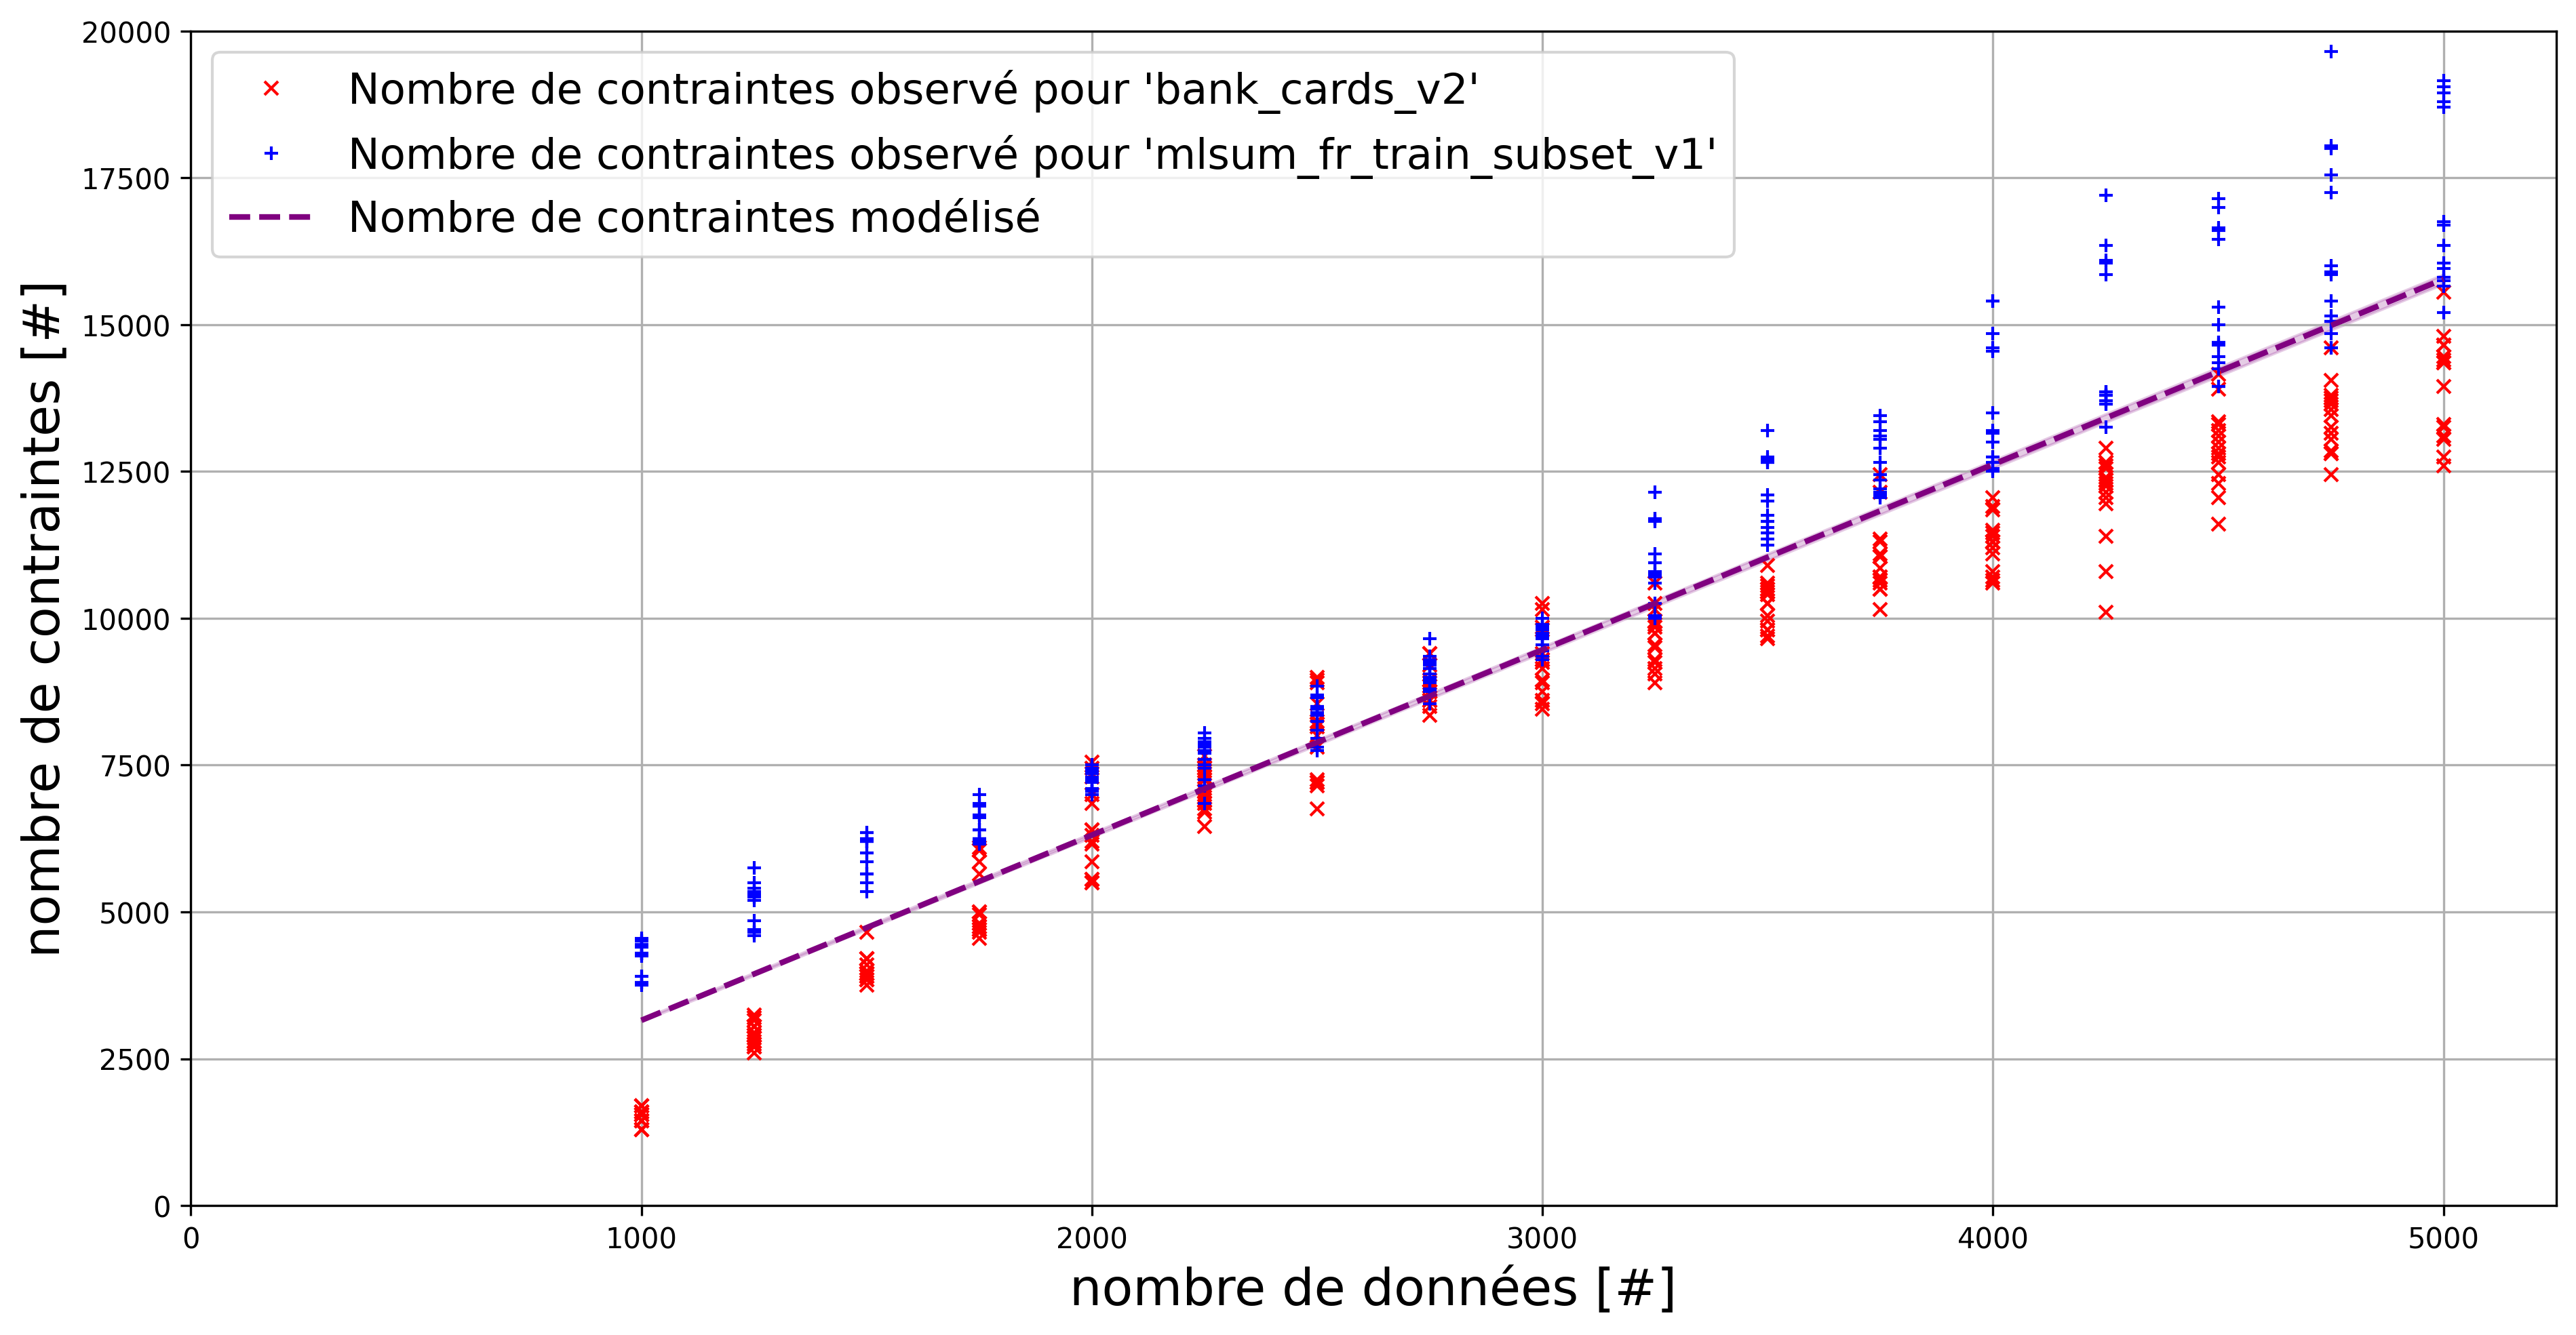
\includegraphics[width=0.95\textwidth]{figures/etude-nombre-contraintes-1-modelisation-nombre}
				\caption{
					Estimation du nombre moyen de contraintes nécessaires à notre \textbf{paramétrage favori} du \texttt{Clustering Interactif} afin d'obtenir une annotation partielle (\textit{atteindre une \texttt{v-measure} de $90$\%}) en fonction de la taille du jeu de données à modéliser.
				}
				\label{figure:4.3.3-ETUDE-COUT-NOMBRE-CONTRAINTES}
			\end{figure}
		
			% Note de l'auteur.
			\begin{leftBarAuthorOpinion}
				% Estimation de points de références.
				Nous pouvons considérer les points de références suivants :
				\begin{itemize}
					\item le nombre de contraintes possibles (avec doublons) est de $\texttt{dataset\_size}^{\textbf{2}}$ (\textit{caractériser chaque couple de données présent dans la matrice d'adjacence}) ;
					\item le nombre de contraintes possibles (sans doublons) est de $\frac{1}{2} \cdot (\texttt{dataset\_size}^{\textbf{2}} - \texttt{dataset\_size})$ (\textit{considérer la symétrie des contraintes, donc seul le triangle supérieur de la matrice d'adjacence a besoin d'être renseigné}) ;
					\item le nombre minimal de contraintes à annoter pour être exhaustif sur une partition en $k$ \textit{clusters} $\{K_{1}, K_{2}, ..., K_{k}\} $ est estimé à ${\displaystyle \sum\limits_{1 \leq i \leq k}{(\|K_{i}\|-1)} + \sum\limits_{1 \leq i \leq k}{(k-i)}} $
					(\textit{il faut d'abord considérer les chemins minimaux pour parcourir les composants connexes avec des contraintes \texttt{MUST-LINK}, correspondant à $\|K_{i}\|-1$ contraintes \texttt{MUST-LINK} pour chaque partition $\|K_{i}\|$, puis ajouter le nombre minimal des contraintes \texttt{CANNOT-LINK} pour distinguer chacun de ses composants connexes en \textit{cluster}}, correspondant au nombre d'arrangements sans répétition de deux partitions).
				\end{itemize}
				%
				% Annonce de la figure.
				La \textsc{Figure~\ref{figure:4.3.3-ETUDE-COUT-NOMBRE-CONTRAINTES-EXEMPLES}} illustre ces propos sur un jeu d'exemples comportant $10$ points de données réparties en $3$ classes, et met en avant l'explosion du nombre de contraintes possible même sur un petit jeu de données (cf.~\ref{figure:4.3.3-ETUDE-COUT-NOMBRE-CONTRAINTES-EXEMPLES}~\textbf{(2)}).
				
				% Application de ces points de référence.
				Avec ces références, le nombre de contraintes est borné approximativement
				entre $1~035$ et $499~500$ pour un jeu de $1~000$ données équilibré en $10$ classes,
				et entre $6~175$ et $12~497~500$ pour un jeu de $5~000$ données équilibré en $50$ classes.
				%
				\begin{figure}[H]
					\centering
					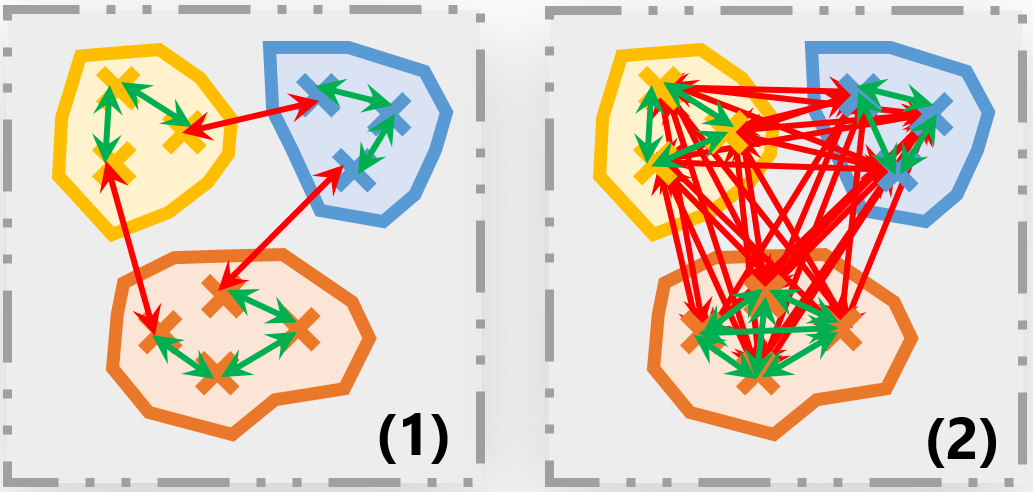
\includegraphics[width=0.5\textwidth]{figures/etude-nombre-contraintes-2-bornes-limites}
					\caption{
						Exemple de caractérisation exhaustive d'un jeu de données ($10$ données, $3$ classes) en ajoutant un nombre minimal de contraintes (cf. \textbf{(1)}) ou en ajoutant toutes les contraintes possibles (cf. \textbf{(2)}).
					}
					\label{figure:4.3.3-ETUDE-COUT-NOMBRE-CONTRAINTES-EXEMPLES}
				\end{figure}
			\end{leftBarAuthorOpinion}

		%%% Discussion.
		\subsubsection{Discussion}
		
			% Rappel de l'objectif.
			L'objectif de cette étude était de déterminer le nombre moyen de contraintes à devoir annoter pour modéliser un jeu de données pour un accord $90$\% de \texttt{v-measure} avec la vérité terrain utilisée.
			Cette estimation, dépendant de la taille du jeu de données manipulé, est représentée par l'\textsc{Equation~\ref{equation:4.3.3-ETUDE-COUT-NOMBRE-CONTRAINTES}}.
			\\
			
			% Discussion générale sur la pente.
			Nous pouvons constater que la relation entre la taille du jeu de données et le nombre de contraintes à annoter est linéaire (pente de $3.15$) : doubler la taille d'un jeu de données doublera donc la charge de travail incombant à l'expert métier.
			À première vue, une telle estimation représente une lourde charge d'annotation : \textbf{pour un jeu de $5~000$ données, il faut caractériser $15~750$ contraintes, ce qui correspond environ à $34$ heures d'annotation} d'après l'\textsc{Equation~\ref{equation:4.3.1-ETUDE-COUT-COUTS-TEMPS-ANNOTATION}} !
			Néanmoins, comme le nombre de contraintes possibles évolue en $ \mathcal{O}(\texttt{dataset\_size}) $, cette estimation aurait pu être bien pire et représenter $12~497~500$ contraintes (cf. \textsc{Figure~\ref{figure:4.3.3-ETUDE-COUT-NOMBRE-CONTRAINTES-EXEMPLES}}).
			Mieux encore, le nombre théorique minimal moyen de contraintes à annoter pour $5~000$ données n'est que $2.55$ fois plus faible que notre estimation ($6~175$ vs $15~750$), alors que cette borne minimale nécessite un échantillonnage "\textit{parfait}" permettant d'identifier le chemin minimal parcourant les \textit{clusters}.
			Nous pouvons donc relativiser l'estimation faite avec l'\textsc{Equation~\ref{equation:4.3.3-ETUDE-COUT-NOMBRE-CONTRAINTES}} et en conclure que notre méthode comporte un nombre de contraintes raisonnable à annoter.
			
			% Influence du jeu de données.
			Bien évidemment, une telle estimation est sensible au jeu de données utilisé comme référence (cf. \textsc{Figure~\ref{figure:4.3.3-ETUDE-COUT-NOMBRE-CONTRAINTES}}).
			Ici, la différence de pente mesurée est de $0.25$ (\texttt{p-valeur}: $> 0.999$), soit un écart moyen d'environ $8$\% par rapport à la modélisation moyenne.
			Toutefois, comme l'impact semble limité, nous maintenons la modélisation moyenne représentée par l'\textsc{Equation~\ref{equation:4.3.3-ETUDE-COUT-NOMBRE-CONTRAINTES}} pour la suite de nos estimations de coûts.
		
			% Note de l'auteur.
			\begin{leftBarAuthorOpinion}
				Il n'y a pas davantage de matière à discussion pour cette étude, car le principal résultat (l'\textsc{Equation~\ref{equation:4.3.3-ETUDE-COUT-NOMBRE-CONTRAINTES}}) est un résultat temporaire nécessaire à l'estimation du coût global d'un projet utilisant une méthodologie de \texttt{Clustering Interactif}.
			\end{leftBarAuthorOpinion}
	
	%%%
	%%% Subsection 4.3.4: Estimation du temps total d'un projet d'annotation en combinant les précédentes études de coûts
	%%%
	\subsection{Estimation du temps total d'un projet d'annotation en combinant les précédentes études de coûts}
	\label{section:4.3.4-ETUDE-COUTS-TOTAL}
	
		% Equation finale.
		Résumons l'ensemble des modélisations réalisées lors des précédentes études (cf. sections \ref{section:4.3.1-ETUDE-COUTS-TEMPS-ANNOTATION}, \ref{section:4.3.2-ETUDE-COUTS-TEMPS-CALCUL} et \ref{section:4.3.3-ETUDE-COUT-NOMBRE-CONTRAINTES}) afin d'estimer le coût total d'un projet d'annotation employant une méthodologie basée sur le \texttt{Clustering Interactif} et utilisant notre \textbf{paramétrage favori} \footnote{
			Paramétrage favori (atteindre $90$\% de \texttt{v-measure} avec un coût minimal): prétraitements simples (\texttt{prep.simple}), vectorisation \texttt{TF-IDF} (\texttt{vect.tfidf}), \textit{clustering} \texttt{KMeans} avec modèle \texttt{COP} (\texttt{clust.kmeans.cop}) et échantillonnage des données les plus proches dans des \textit{clusters} différents (\texttt{sampl.closest.diff}).
		}.
		Dans les notations, $\texttt{dataset\_size}$ représente la taille du jeu de données à modéliser, et $\texttt{batch\_size}$ représente le nombre de contraintes que l'expert annote à chaque itération.

		%%% Résultats.
		\subsubsection{Synthèse des résultats}
			
			% Equation: Temps pour une itération (séquentielle).
			Tout d'abord, nous pouvons estimer le \textbf{temps moyen d'une itération de la méthode}, comprenant d'une part les temps d'exécution des algorithmes (\textit{prétraitements}, \textit{vectorisation}, \textit{clustering}, \textit{échantillonnage}) et d'autre part le temps d'annotation d'un lot de contraintes, grâce aux équations suivantes :
			\begin{equation}
				\label{equation:4.3.4-ETUDE-COUT-UNE-ITERATION-SEQUENTIELLE}
				\begin{cases}
					% Computation time.
					\texttt{computation\_time}~[s]&
						~\propto~0.17 \cdot \texttt{dataset\_size}\\
					% Annotation time.
					\texttt{annotation\_time}~[s]&
						~\propto~7.8 \cdot \texttt{batch\_size} \\
					% One iteration time (sequential).
					\texttt{iteration\_time(sequential)}~[s]&
						~\propto~\texttt{computation\_time} + \texttt{annotation\_time} \\
				\end{cases}
			\end{equation}
			
			% Equation: Nombre d'itérations (séquentielle).
			Ensuite, nous sommes en mesure d'anticiper le \textbf{nombre moyen de contraintes à annoter} pour modéliser le jeu de données avec un seuil de $90$\% de \texttt{v-measure}, et donc de déduire le nombre d'itérations nécessaire de la méthode, grâce aux équations suivantes :
			\begin{equation}
				\label{equation:4.3.4-ETUDE-COUT-NOMBRE-ITERATIONS-SEQUENTIEL}
				\begin{cases}
					% Constraints number.
					\texttt{constraints\_needed}~[\#] &
						~\propto~3.15 \cdot \texttt{dataset\_size} \\
					% Iterations number.
					\texttt{iterations\_needed}~[\#] &
						~\propto~\frac{\texttt{nb\_constraints}}{\texttt{batch\_size}} \\
				\end{cases}
			\end{equation}
			
			% Equation: Temps total pour un projet (séquentielle).
			Enfin, il suffit de combiner \textsc{Equation~\ref{equation:4.3.4-ETUDE-COUT-UNE-ITERATION-SEQUENTIELLE}} et \textsc{Equation~\ref{equation:4.3.4-ETUDE-COUT-NOMBRE-ITERATIONS-SEQUENTIEL}} pour estimer le temps total nécessaire à un projet d'annotation utilisant le \texttt{Clustering Interactif} (c'est-à-dire en enchaînant successivement des étapes d'échantillonnage, d'annotation et de \textit{clustering}, cf. \textsc{Figure~\ref{figure:4.3.4-ETUDE-COUT-TOTAL-ARCHITECTURE}} (1)) pour converger vers $90$\% de \texttt{v-measure} :
			\begin{equation}
				\label{equation:4.3.4-ETUDE-COUT-TOTAL-SEQUENTIEL}
				\begin{cases}
					% Total time (sequential).
					\texttt{total\_time(sequential)}~[s] &
						~\propto~\texttt{iteration\_time} \cdot \texttt{iterations\_needed}
				\end{cases}
			\end{equation}
			
			% Figure.
			Ces estimations globales sont représentées sur la \textsc{Figure~\ref{figure:4.3.4-ETUDE-COUT-TOTAL}} en fonction de plusieurs tailles de jeu de données et plusieurs tailles de lots d'annotation.

		%%% Discussion finale.
		\subsubsection{Discussion du coût total}
		
			% Rappel des objectifs.
			L'objectif de cette section consistait à déterminer les coûts relatifs à la tâche d'annotation de contraintes par un expert métier et au temps d'exécution des algorithmes intervenant dans notre implémentation du \texttt{Clustering Interactif}.
			Pour cela, nous avons chronométré des annotateurs en situation réelle (cf. \textsc{Section~\ref{section:4.3.1-ETUDE-COUTS-TEMPS-ANNOTATION}}), estimé le temps de calcul de chaque algorithme implémenté (cf. \textsc{Section~\ref{section:4.3.2-ETUDE-COUTS-TEMPS-CALCUL}}) et trouvé le moyen de prédire le nombre de contraintes à annoter sur un jeu de données (cf. \textsc{Section~\ref{section:4.3.3-ETUDE-COUT-NOMBRE-CONTRAINTES}}).
			Nous avons pu montrer qu'une annotation de contraintes est plus rapide qu'une annotation par label et nous conseillons, d'après notre analyse empirique, des sessions d'annotation de moins de $150$ contraintes pour ne pas épuiser l'annotateur.
			Sur le paramétrage de la méthode, nous avons rejeté l'usage d'algorithmes de \textit{clustering} de type hiérarchique à cause de leur lenteur, au profit du \texttt{KMeans} avec modèle \texttt{COP} (\texttt{clust.kmeans.cop}).
			Notre paramétrage favori, permettant d'atteindre $90$\% de \texttt{v-measure} avec un coût minimal, est ainsi constitué des prétraitements simples (\texttt{prep.simple}), d'une vectorisation \texttt{TF-IDF} (\texttt{vect.tfidf}), d'un \textit{clustering} \texttt{KMeans} avec modèle \texttt{COP} (\texttt{clust.kmeans.cop}) et d'un échantillonnage des données les plus proches dans des \textit{clusters} différents (\texttt{sampl.closest.diff}).
			Enfin, pour atteindre cet objectif de \texttt{v-measure}, le nombre moyen de contraintes à annoter avec notre méthodologie semble rester linéairement proportionnel à la taille du jeu de données à modéliser, ce qui est encourageant au regard de la combinatoire de contraintes possibles.
			\\
			
			% Annonce des résultats : c'est long !
			La mise en commun de ces résultats se retrouve dans \textsc{Equation~\ref{equation:4.3.4-ETUDE-COUT-UNE-ITERATION-SEQUENTIELLE}}, \textsc{Equation~\ref{equation:4.3.4-ETUDE-COUT-NOMBRE-ITERATIONS-SEQUENTIEL}} et \textsc{Equation~\ref{equation:4.3.4-ETUDE-COUT-TOTAL-SEQUENTIEL}}.
			Comme le nombre de données à annoter est inversement proportionnel au nombre d'itérations à réaliser, nous avons le dilemme suivant : soit nous annotons de petits lots ($50$ contraintes) pour rapidement intégrer les contraintes et permettre à l'annotateur de se reposer régulièrement (\textit{mais ce dernier va en contrepartie devoir attendre plus souvent la fin des exécutions du \textit{clustering}}) soit nous annotons des lots plus conséquents ($150$ contraintes) pour diminuer le nombre d'itérations et exécuter moins de \textit{clustering}, (\textit{mais cela risque d'épuiser l'opérateur avec des grosses charges d'annotations}).
			Dans les deux cas, \textbf{le coût total semble élevé} : pour un jeu de $5~000$ points de données, et avec des tailles d'échantillons comprises entre $50$ et $150$ contraintes, il faut entre $59$ et $110$ heures de travail (\textit{$34$ heures d'annotations et entre $25$ et $76$ heures d'attente de la fin d'exécution d'algorithmes suivant la taille des lots}).
			En considérant une journée de travail de $7$ heures, cela représente une charge contenue entre $8.4$ et $15.7$ jours pour avoir un jeu de donnée fiable à $90$\% de \texttt{v-measure}.
			Pour finir, nous ajoutons $1$ jour pour combler l'écart théorique de $10$\% de \texttt{v-measure} en corrigeant manuellement le résultat obtenu, et $1$ jour supplémentaire pour interpréter et nommer chaque \textit{cluster} (voir \textsc{Algorithme~\ref{algorithm:3.2-CLUSTERING-INTERACTIF}}, \textit{ligne 13}).
			Au final, pour un ensemble de $5~000$ données, il faut donc entre $8.4$ {\footnotesize $(+2)$} et $15.7$ {\footnotesize $(+2)$} jours de travail à un expert métier pour obtenir une base d'apprentissage avec une méthodologie basée sur le \texttt{Clustering Interactif}.
			
			% Critique du résultat : comparaison avec une annotation classique, avoir plusieurs annotateurs, ...
			Pour critiquer l'approximation que nous avons faite lors de cette section, nous essayons de comparer le temps nécessaire qu'il aurait fallu à un projet d'annotation traditionnel, comme décrit en \textsc{Section~\ref{section:2.2.1-ORGANISATION-ANNOTATION-ETAPES-CLES}} (cycle \texttt{MATTER}), et notre proposition de cycle d'annotation avec le \texttt{Clustering Interactif}, visible en \textsc{Figure~\ref{figure:4.3.4-ETUDE-COUT-TOTAL-ARCHITECTURE}} (1).
			En nous basant sur un ensemble de $5~000$ données à annoter, nous estimons qu'il faut :
			$1$ jour de travail pour définir une représentation des données en modèle de classification ;
			$4$ jours de travail pour annoter $5~000$ données (à raison de $20$ secondes par données, estimation haute inspirée de \cite{pradhan-etal:2007:semeval2007-task-17} où la "\textit{désambiguïsation du sens des mots}", présentée comme une tâche de classification, demande $17.5$ secondes par données) ;
			$2$ jours de marge d'erreur pour changer de modèle de représentation s'il ne semble pas adapté aux données en cours d'annotation.
			Au total, nous estimons donc qu'il faut $5$ {\footnotesize $(+2)$} jours de travail \footnote{
				$5$ {\footnotesize $(+2)$} jours de travail : Notons que cette estimation n'est bien entendu pas généralisable.
				En effet, le temps nécessaire aux phases de modélisation et de revues peut fortement augmenter si le cas d'usage est plus complexe.
				Par exemple, la classification de questions en une centaine d'intentions peut prendre plusieurs jours voire quelques semaines d'étude alors que la classification de sentiments sur trois niveaux (positif, négatif, neutre) est presque triviale.
			} à un expert métier pour obtenir une base d'apprentissage avec une méthodologie traditionnelle.
			\textbf{En l'état, nous pouvons donc conclure que le \texttt{Clustering Interactif} que nous proposons est en moyenne deux fois plus coûteux qu'une annotation manuelle classique ($8.4$ {\footnotesize $(+2)$} à $15.7$ {\footnotesize $(+2)$} jours vs $5$ {\footnotesize $(+2)$} jours), ce qui peut être un frein à son utilisation en situation réelle}.
			
			% Pistes d'amélioration : Augmenter la taille des lots d'annotation + Augmenter le nombre d'annotateurs + paralléliser annotation et \textit{clustering}, ...
			Afin d'accélérer la phase d'annotation et de diminuer le nombre d'itérations, il est bien entendu possible d'augmenter la taille des échantillons de contraintes à annoter ou d'ajouter plusieurs opérateurs.
			Cependant, une telle solution ne permet toujours pas d'être compétitif avec l'annotation traditionnelle si cette dernière dispose aussi de plusieurs opérateurs (\textit{avec $2$ annotateurs : de $6.5$ {\footnotesize $(+2)$} à $13.3$ {\footnotesize $(+2)$} jours vs $3$ {\footnotesize $(+2)$} jours ; avec $4$ annotateurs : de $4.8$ {\footnotesize $(+2)$} à $12.1$ {\footnotesize $(+2)$} jours vs $2$ {\footnotesize $(+2)$} jours}).
			Une autre piste, plus prometteuse, consiste plutôt à adapter notre méthode pour exploiter les temps d'attente lors de l'exécution d'un \textit{clustering}.
			

		%%% Ouverture
		\subsection{Ouverture vers une annotation en parallèle du \textit{clustering}}
		
			% Idée : Optimiser le temps d'attente.
			Notre méthodologie d'annotation basée sur le \texttt{Clustering Interactif} est pénalisée par la séquentialité des actions à réaliser.
			En effet, l'annotateur doit attendre la fin de l'exécution des algorithmes de \textit{clustering} et d'échantillonnage avant de pouvoir travailler.
			D'après nos précédentes estimations sur un jeu de $5~000$ données, l'opérateur doit attendre entre $25$ et $76$ heures en fonction de la taille de lots d'annotation choisie, et une idée à explorer consiste à optimiser ce temps d'attente.
			
			% Réalisation : Paralléliser annotation et \textit{clustering} !
			L'amélioration envisagée consiste à \textbf{réaliser l'annotation de contraintes en parallèle de l'exécution du \textit{clustering}}, comme représenté dans la \textsc{Figure~\ref{figure:4.3.4-ETUDE-COUT-TOTAL-ARCHITECTURE}} (2).
			Dans cette version, l'échantillonnage se base toujours sur le résultat du \textit{clustering} de l'itération précédente, mais le \textit{clustering} intègre les contraintes annotées avec un décalage d'une itération.
			Un tel changement permet de limiter le temps d'attente de l'opérateur et d'optimiser l'enchaînement des algorithmes.

			% Figure architecture.
			\begin{figure}[!htb]
				\centering
				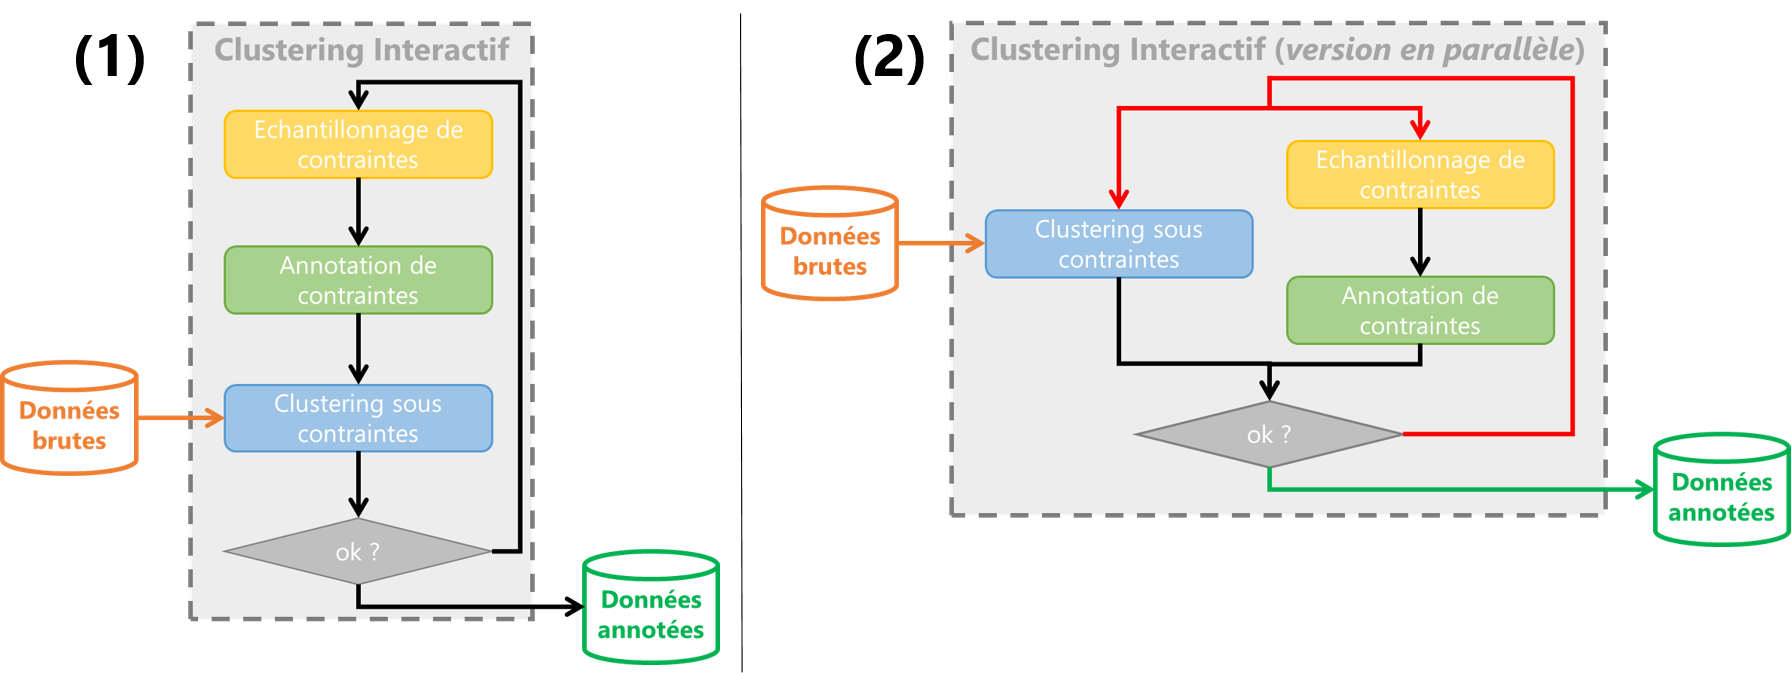
\includegraphics[width=0.95\textwidth]{figures/interactive-clustering-architecture-sequentielle-vs-parallele}
				\caption{
					Schéma comparatif des architectures du \texttt{Clustering Interactif} : \textbf{(1)} représente la version séquentielle initialement présentée en \textsc{Chapitre~\ref{chapter:3-CLUSTERING-INTERACTIF}} où le \textit{clustering} s'adapte avec les annotations de l'itération en cours ; \textbf{(2)} représente l'évolution en mode \textit{parallèle} où le \textit{clustering} s'adapte avec les annotations de l'itération précédente (décalage d'une itération).
				}
				\label{figure:4.3.4-ETUDE-COUT-TOTAL-ARCHITECTURE}
			\end{figure}
			
			% Equation : Adaptation du Temps pour une itération (parallèle).
			Avec cette version, le temps nécessaire à une itération correspond à la durée la plus longue entre le temps d'annotation et le temps de calcul des algorithmes.
			Nous pouvons donc adapter l'\textsc{Equation~\ref{equation:4.3.4-ETUDE-COUT-UNE-ITERATION-SEQUENTIELLE}} par l'équation suivante :
			\begin{equation}
				\label{equation:4.3.4-ETUDE-COUT-UNE-ITERATION-PARALLELE}
				\begin{cases}
					% Computation time.
					\texttt{computation\_time}~[s]&
						~\propto~0.17 \cdot \texttt{dataset\_size}\\
					% Annotation time.
					\texttt{annotation\_time}~[s]&
						~\propto~7.8 \cdot \texttt{batch\_size} \\
					% One iteration time (parallel).
					\texttt{iteration\_time(parallel)}~[s]&
						~\propto~max(\texttt{computation\_time}, \texttt{annotation\_time}) \\
				\end{cases}
			\end{equation}
			
			% Equation : Adaptation du Nombre d'itérations (parallèle).
			Ensuite, afin de limiter les pertes de temps (humain et machine), nous pouvons choisir une taille de lot d'annotations rendant ces deux durées équivalentes.
			Nous déduisons donc les changements suivants dans l'\textsc{Equation~\ref{equation:4.3.4-ETUDE-COUT-NOMBRE-ITERATIONS-SEQUENTIEL}} :
			\begin{equation}
				\label{equation:4.3.4-ETUDE-COUT-NOMBRE-ITERATIONS-PARALLELE}
				\begin{cases}
				\begin{aligned}
					% Batch size.
					\texttt{optimal\_batch\_size}~[\#]&
						~\propto~\frac{\texttt{computation\_time}}{7.8}&
						~\propto~0.0218 \cdot \texttt{dataset\_size} \\
					% Iterations number.
					\texttt{iterations\_needed}~[\#] &
						~\propto~\frac{\texttt{nb\_constraints}}{\texttt{optimal\_batch\_size}}&
						~\propto~144.5 \\
				\end{aligned}
				\end{cases}
			\end{equation}
			
			% Equation: Adaptation du Temps total pour un projet (parallèle).
			Enfin, il suffit de combiner \textsc{Equation~\ref{equation:4.3.4-ETUDE-COUT-UNE-ITERATION-PARALLELE}} et \textsc{Equation~\ref{equation:4.3.4-ETUDE-COUT-NOMBRE-ITERATIONS-PARALLELE}} pour estimer le temps total nécessaire à un projet d'annotation pour converger vers $90$\% de \texttt{v-measure} utilisant la version parallèle du \texttt{Clustering Interactif} :
			\begin{equation}
				\label{equation:4.3.4-ETUDE-COUT-TOTAL-PARALLELE}
				\begin{cases}
					% Total time (parallel).
					\texttt{total\_time(parallel)}~[s] &
						~\propto~\texttt{iteration\_time} \cdot \texttt{iterations\_needed} \\
					\texttt{total\_time(parallel)}~[s] &
						~\propto~24.6 \cdot \texttt{dataset\_size}
				\end{cases}
			\end{equation}
			
			% Figure.
			Ces estimations mises à jour sont représentées sur la \textsc{Figure~\ref{figure:4.3.4-ETUDE-COUT-TOTAL}} en fonction de plusieurs taille de jeu de données, et permettent de faire la comparaison avec la version séquentielle initialement présentée.
			
			% Figures.
			%
			\begin{figure}[!htb]
				\centering
				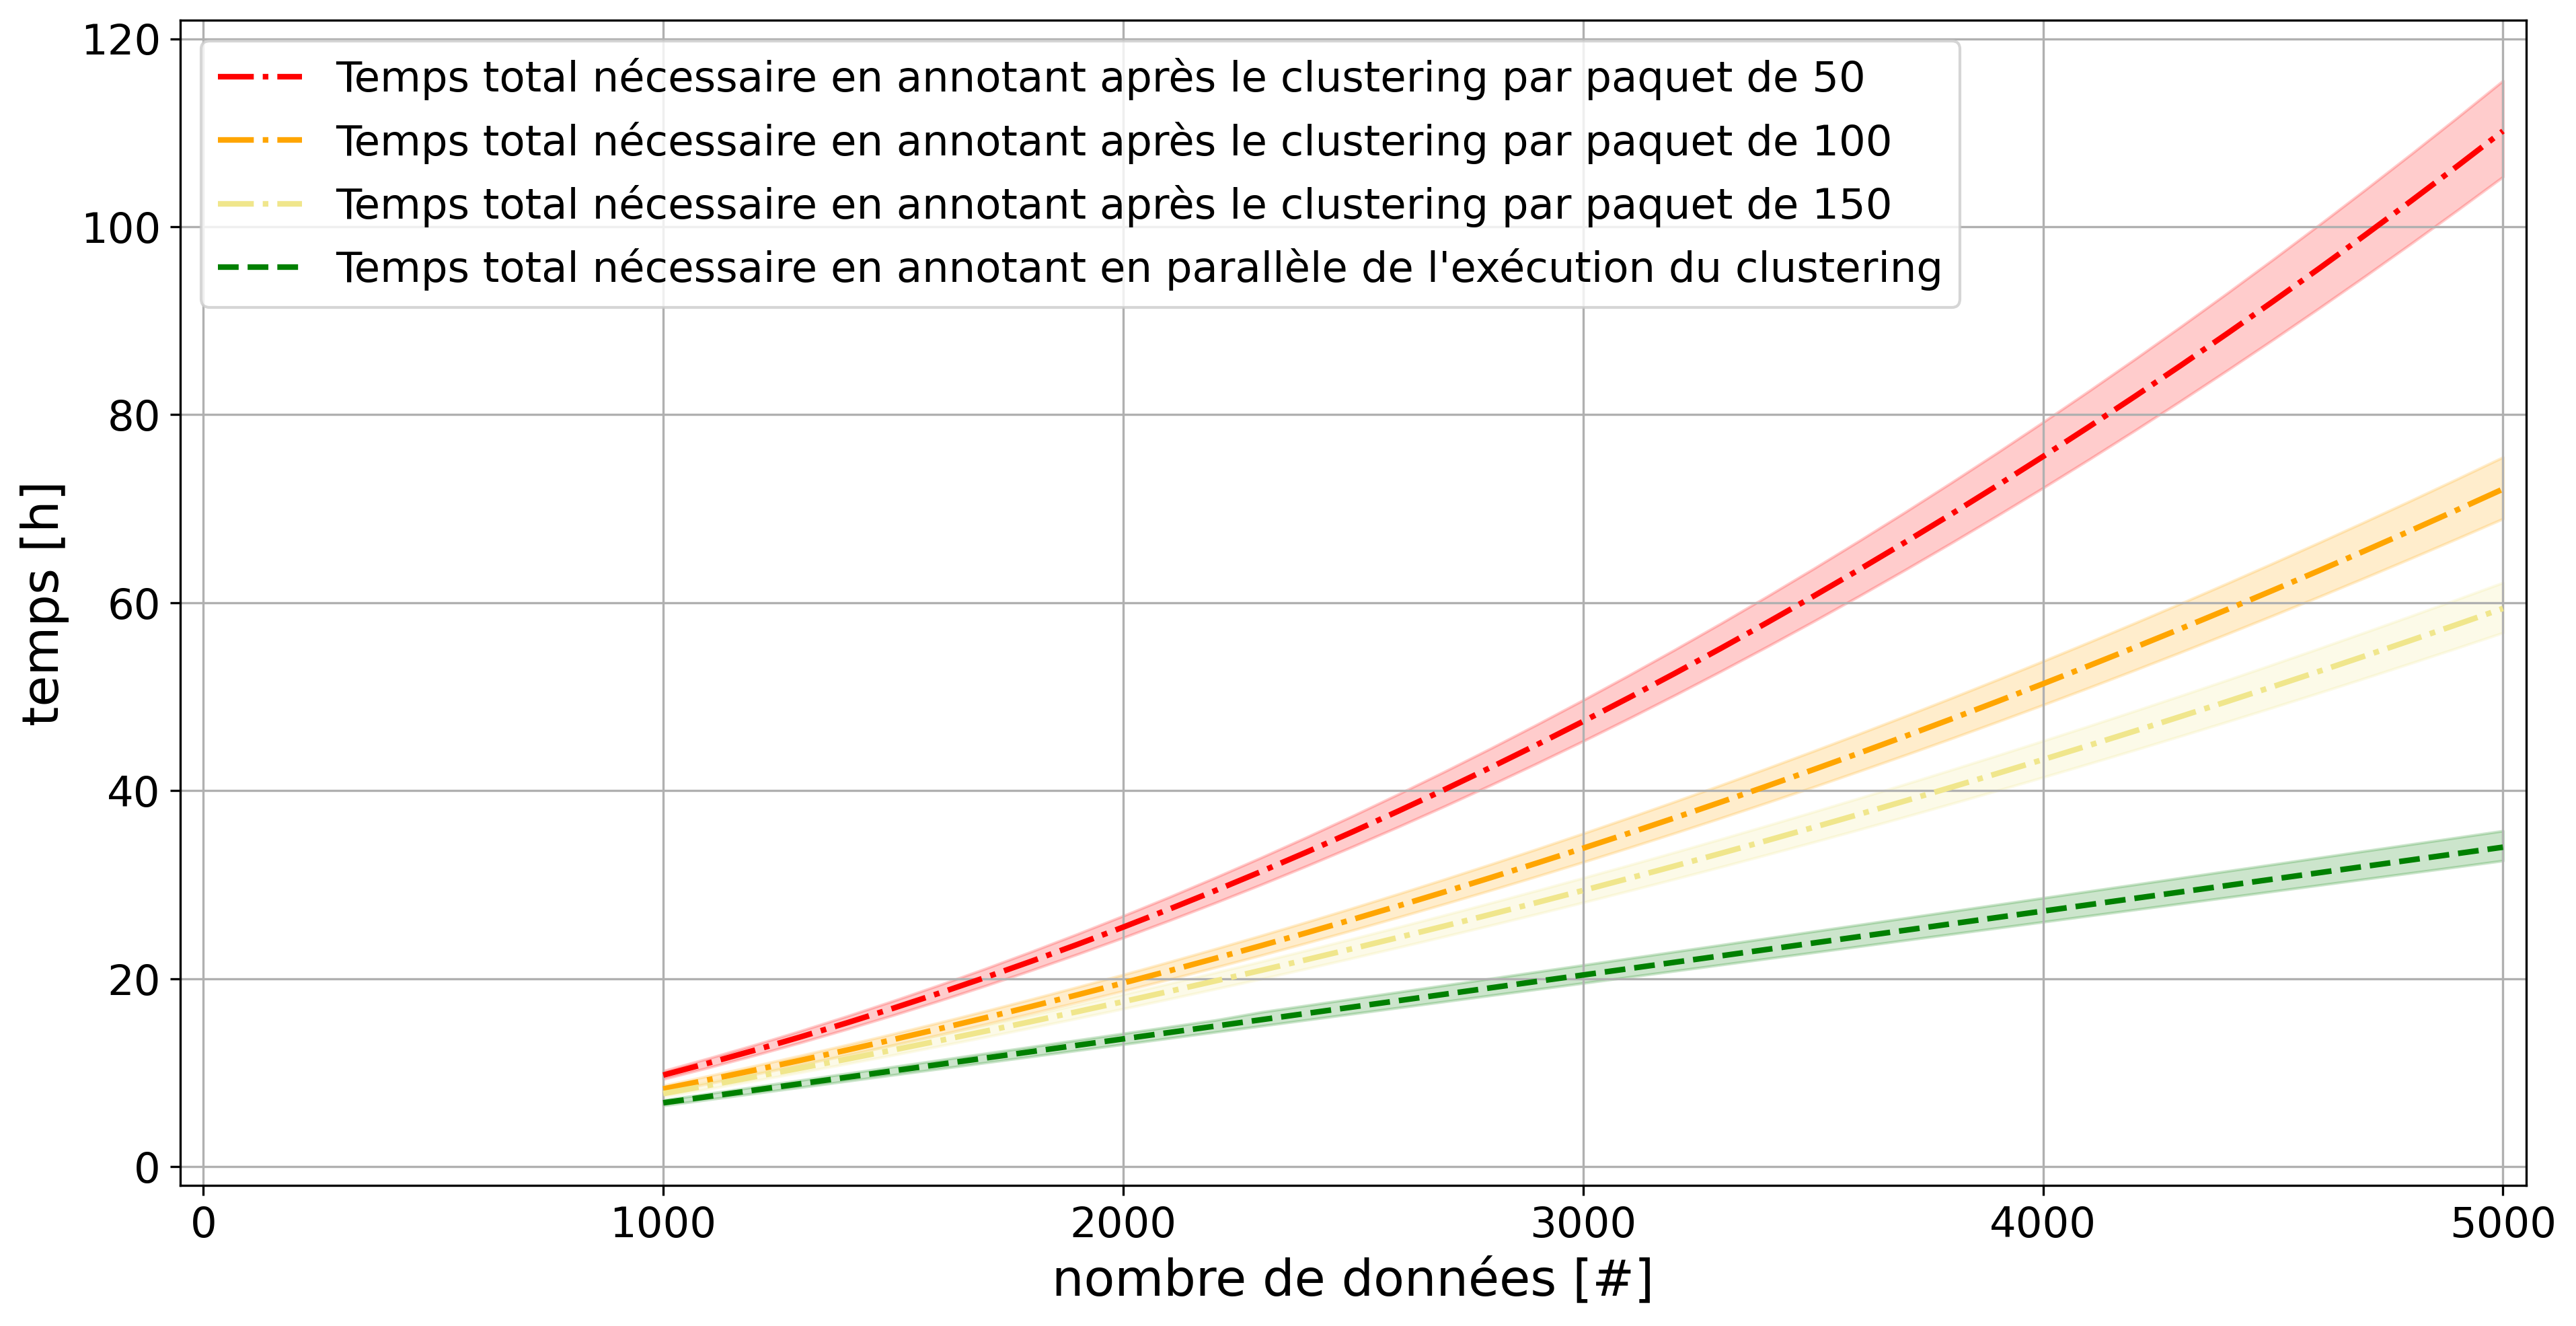
\includegraphics[width=0.95\textwidth]{figures/etude-temps-total-2-modelisation-parallele}
				\caption{
					Estimation du temps total nécessaire (en heures) pour modéliser un jeu de données avec notre \textbf{paramétrage favori} du \texttt{Clustering Interactif} afin d'obtenir une annotation partielle (\textit{atteindre une \texttt{v-measure} de $90$\%}), en fonction de plusieurs tailles de jeu de données, plusieurs tailles de lots d'annotation, et mettant en opposition l'approche séquentielle (\textit{annotation puis le \textit{clustering}}) et l'approche parallèle (\textit{annotation pendant le \textit{clustering}}).
				}
				\label{figure:4.3.4-ETUDE-COUT-TOTAL}
			\end{figure}
			
			% Résultats et discussion : linéaire, 25 x dataset size : c'est acceptable !
			Nous pouvons déjà remarquer que le coût d'annotation du projet devient linéaire en nombre de données (pente de $24.6$ secondes) et nécessite un nombre fixe de $145$ itérations.
			En reprenant une base de $5~000$ données et une marge de $2$ jours pour corriger et nommer les \textit{clusters} \footnote{
				Nommer les \textit{clusters} : voir \textsc{Algorithme~\ref{algorithm:3.2-CLUSTERING-INTERACTIF}}, \textit{ligne 13}.
			}, cela représente $4.8$ {\footnotesize $(+2)$} jours de travail, un estimation équivalente à une annotation traditionnelle qui nécessite $5 $ {\footnotesize $(+2)$} jours de travail d'après nos approximations.
			De plus, si nous ajoutons plusieurs opérateurs, cette version parallèle reste compétitive (\textit{avec $2$ annotateurs : $2.5$ {\footnotesize $(+2)$} jours vs $3$ {\footnotesize $(+2)$} jours ; avec $4$ annotateurs : $1.3$ jours vs $2$ {\footnotesize $(+2)$} jours}).
			Cette découverte est très encourageante, car cela confirme qu'une méthodologie basée sur notre implémentation du \texttt{Clustering Interactif} \textbf{permet d'obtenir une base d'apprentissage avec un coût temporel équivalent à un projet traditionnel} utilisant une annotation par label.
			Cette méthode est d'autant plus intéressante qu'elle fait intervenir un mécanisme d'annotation rapide et intuitif pour un expert métier.
			
			% Conclusion.
			\begin{leftBarSummary}
				Au cours de cette étude de coûts, nous avons pu déduire que :
				\begin{itemize}
					\item[\itemok] L'annotation d'une contrainte nécessite en moyenne $8$ secondes : cette tâche est rapide et intuitive (cf. \textsc{Section~\ref{section:4.3.1-ETUDE-COUTS-TEMPS-ANNOTATION}}) ;
					\item[\itemok] Notre paramétrage favori, permettant d'atteindre $90$\% de \texttt{v-measure} avec un coût minimal, est constitué des prétraitements simples (\texttt{prep.simple}), de la vectorisation \texttt{TF-IDF} (\texttt{vect.tfidf}), du \textit{clustering} \texttt{KMeans} avec modèle \texttt{COP} (\texttt{clust.kmeans.cop}) et de l'échantillonnage des données les plus proches dans des \textit{clusters} différents (\texttt{sampl.closest.diff}).
					Ce paramétrage a un coût moyen de $0.17 \cdot \texttt{dataset\_size}$ secondes (cf. \textsc{Section~\ref{section:4.3.2-ETUDE-COUTS-TEMPS-CALCUL}}) ;
					\item[\itemok] Une adaptation optimale de notre méthodologie consiste mettre en parallèle l'exécution du \textit{clustering} avec l'annotation de contraintes afin de limiter les temps d'attente inutiles.
					Une telle méthode a un coût moyen de $24.6 \cdot \texttt{dataset\_size}$ pour atteindre $90$\% de \texttt{v-measure}, auquel nous ajoutons $2$ jours de travail pour raffiner les \textit{clusters} et les nommer.
					Ce temps est compétitif avec une annotation traditionnelle (cf. \textsc{Section~\ref{section:4.3.4-ETUDE-COUTS-TOTAL}}) ;
					\item[\itemok] Cette étude met en avant l'intérêt des interactions homme-machine : (1) l'expert métier se recentre sur son domaine de compétence avec une caractérisation proche de ses connaissances ("\textit{les données sont-elles similaires ?}") et (2) la machine optimise l'intervention de l'expert pour que ce dernier soit toujours pertinent dans ses contributions.
				\end{itemize}
			\end{leftBarSummary}
		
		% Transition: Vers Pertinence et Rentabilité.
		Dans les sections suivantes, nous allons nous intéresser à l'analyse des résultats de cette méthode.
		En effet, en situation réelle, nous n'avons pas accès à la vérité terrain car elle est justement en cours de construction.
		Il nous est donc impossible d'estimer notre seuil de \texttt{v-measure}, et donc incapable de s'arrêter à $90$\% de \texttt{v-measure}.
		Nous nous intéressons donc à l'estimation de la valeur métier d'un résultat de \textit{clustering} (cf. hypothèse de pertinence en \textsc{Section~\ref{section:4.4-HYPOTHESE-PERTINENCE}}) et à la définition de cas d'arrêt indépendants d'une vérité terrain (cf. hypothèse de rentabilité en \textsc{Section~\ref{section:4.5-HYPOTHESE-RENTABILITE}}).